\documentclass[letterpaper,12pt,openany]{book}  
\usepackage[spanish,es-nodecimaldot,es-tabla]{babel}
\usepackage[utf8]{inputenc}  
\usepackage{graphicx} 
\usepackage[svgnames,table]{xcolor}  
\usepackage{ESFMpreamble}  
\usepackage{mypreamble} 
\graphicspath{{img/}}  
\usepackage{csquotes}

\usepackage{amsthm}
\usepackage{amsmath}
\usepackage{fancyhdr}
\pagestyle{fancy}     
\usepackage{comment} 
\usepackage[
backend=biber,
style=alphabetic,
sorting=ynt
]{biblatex}

%\addcontentsline{toc}{chapter}{references.bib}

\addbibresource{references.bib}

 \fancyhf{}
 \fancyhead[LE]{\nouppercase{\leftmark}}
 \fancyhead[RO]{\nouppercase{\rightmark}}
 \lfoot[\thepage]{}
 \rfoot[]{\thepage} 
 \renewcommand{\headrulewidth}{0.5pt}
 \renewcommand{\footrulewidth}{0.5pt} 
 
\author{Luis Donaldo Barreto García}
\documentType{T E S I S} 
\title{Mapeo conforme usando Mathematica}
\degree{LICENCIADO EN FÍSICA Y MATEMÁTICAS\\CON ESPECIALIDAD EN MATEMÁTICAS}
\supervisor{Dr. Luis Manuel Tovar Sánchez}
\cityandyear{Ciudad de México, \today}


%Entornos de definiciones, teoremas, etc.
%
\theoremstyle{definition}
\newtheorem{lema}{Lema}

\theoremstyle{definition}
\newtheorem{prop}{Proposición}


\theoremstyle{definition}
\newtheorem{teor}{Teorema}

\theoremstyle{definition}
\newtheorem{coro}{Corolario}


\newtheorem{ole}{Conjetura}

\theoremstyle{definition}
\newtheorem{defi}{Definición}

\theoremstyle{remark}
\newtheorem*{remark}{Observación}

\theoremstyle{definition}
\newtheorem{Ejem}{Ejemplo}


%Reales, complejos, enteros, naturales.

\newcommand{\R}{\mathbb{R}}
\newcommand{\C}{\mathbb{C}}
\newcommand{\Z}{\mathbb{Z}}
\newcommand{\N}{\mathbb{N}}
\newcommand{\ds}{\displaystyle}
\newcommand{\Ind}{\mbox{Ind}}
\newcommand{\SC}{Schwarz-Christoffel}
\newcommand{\dpartial}[2]{\dfrac{\partial#1}{\partial#2}}
\newcommand{\derivada}[2]{\dfrac{d#1}{d#2}}
\newcommand{\mobius}[4]{\dfrac{#1z#2}{#3z#4}}
\newcommand{\capertura}{``}
\newcommand{\ccierre}{''}

%Demostración
\def\proof{\vspace{-0.5 cm}\paragraph{ Demostraci\'on:}}
\def\endproof{\\\mbox{}\hfill $_\blacksquare$}
\def\solu{\vspace{-0.5 cm}\paragraph{ Soluci\'on:\\}}
\def\endsolu{\\\mbox{}\hfill ${\blacklozenge}$}

%-----------------------------------------------------------------------------%
% Cuerpo
\raggedbottom
\setlength{\parindent}{0pt}


\begin{document}
	
	% Portada
	\maketitle  
	
	\thispagestyle{empty} 
	
	\frontmatter
	
	% Dedicatoria
	\chapter*{}
	\begin{flushright}%
		\emph{¿Dedicatoria? \ldots}
		\thispagestyle{empty}
	\end{flushright}
	
	% Abstract
	\chapter*{Resumen}
	\addcontentsline{toc}{chapter}{Resumen}
	En este trabajo, se muestra cómo podemos utilizar \textbf{Mathematica}, un software de cálculo simbólico, para visualizar el comportamiento gráfico de las funciones complejas, en particular, los mapeos conformes.
	
	En el primer capítulo, presentamos de manera concisa los conceptos de diferenciación compleja, como la regla de la cadena y las ecuaciones de Cauchy-Riemann. Posteriormente, se exponen resultados de la teoría de funciones analíticas, como el Teorema de Identidad para Funciones Analíticas, que establece cuándo dos funciones son iguales en un dominio $\Omega$. Se muestra de manera resumida cómo podemos usar Mathematica para graficar funciones complejas utilizando la función \textbf{ComplexPlot} de Mathematica. Esta forma de graficar funciones nos permite observar ciertos comportamientos alrededor de los polos y singularidades de las funciones complejas. Para finalizar este capítulo, se presenta el Teorema de Ahlfors-Struble. A pesar de su simplicidad, este teorema es de gran ayuda, ya que permite obtener una función analítica a partir de su componente real (o compleja), y lo más sorprendente es que nos permite encontrar la función analítica de manera algebraica.
	
	En el segundo capítulo, comenzamos definiendo lo que es un mapeo conforme. Posteriormente, se ilustra cómo podemos usar Mathematica para graficar algunas funciones elementales, esta vez utilizando otra forma de graficar las funciones de variable compleja, que nos permite ver cómo se deforma el plano complejo bajo tales funciones. Luego, se estudian las transformaciones de Möbius, el mapeo de Joukowski y el mapeo de Schwarz-Christoffel. Usamos Mathematica para ver la deformación del plano complejo $\C$ o dominios $\Omega\subset\C$ así como para realizar cálculos de integrales que dan como resultado funciones hipergeométricas, las cuales ya vienen incluidas en Mathematica y nos ahorran esfuerzo y tiempo al calcularlas usando dicho software.
	
	Finalmente, en el tercer capítulo, se presentan algunos ejemplos que ilustran el uso de los mapeos conformes en problemas de física. Estos pueden resultar interesantes para los físicos e ingenieros al momento de estudiar problemas relacionados con el flujo de fluidos, la transferencia de calor o el campo electromagnético.
	% palabras clave
	%\paragraph{Palabras clave:} 
	% Abstract
	% Agradecimientos
	\chapter*{Agradecimientos}
	\addcontentsline{toc}{chapter}{Agradecimientos}
	
	Por redactar \ldots
	
	% Tabla de contenidos
	\tableofcontents
	 
	\listoffigures
	
	\chapter*{Introducción}
	\addcontentsline{toc}{chapter}{Introducción}
	Un mapeo conforme, en términos generales, es una función que preserva ángulos. Este tipo de mapeos tiene una gran importancia en la física, en áreas como el flujo de fluidos, la transferencia de calor y la acústica. Estos mapeos se estudian en cursos introductorios de variable compleja, donde se presentan algunos resultados relacionados con ellos. Sin embargo, a menudo se descuida la parte visual. En cursos como cálculo diferencial e integral de una o varias variables, podemos visualizar el comportamiento gráfico de las funciones. Esta visualización es de gran ayuda, ya que permite un análisis más detallado del comportamiento de las funciones de variable real (siempre que la suma de las dimensiones del codominio y el dominio sea menor o igual a tres). Sin embargo, para el caso de funciones de variable compleja, necesitaríamos un espacio en cuatro dimensiones para graficar estas funciones, lo cual resulta imposible para nosotros. No obstante, podemos obtener ciertas representaciones gráficas con la ayuda de una computadora, lo cual nos permite estudiar un poco más a fondo las funciones de variable compleja.
	
	El principal motivo para la elaboración de este trabajo es ilustrar el uso de Mathematica, un software de cálculo simbólico, para la representación gráfica de funciones de variable compleja, principalmente los mapeos conformes y cómo estos deforman el plano complejo. También se presentan ejemplos de cómo usar Mathematica para realizar cálculos numéricos y simbólicos de integrales, lo que resulta más práctico que realizar el cálculo a mano. Por lo tanto, se pretende que este trabajo sea utilizado como un complemento a los cursos de variable compleja. Por tal motivo, se espera que el lector tenga conocimientos de los temas que se suelen ver en estos cursos, ya que por eso mismo omitimos las demostraciones y solo referenciamos los textos donde el lector pueda encontrar las pruebas de los teoremas y proposiciones que se incluyen en este escrito, con el fin de centrarnos más en la ilustración de funciones complejas con la ayuda de Mathematica.
	
	Este trabajo está fuertemente influenciado por los cursos de variable compleja que se imparten en la Escuela Superior de Física y Matemáticas, así como en \cite{shaw} y \cite{silverman}. Cabe mencionar que Mathematica tiene una extensa documentación en internet, la cual se encuentra disponible para su consulta en la web \url{https://www.wolfram.com/}.
	% Capitulos
	\mainmatter
	
	\spacing{1.1}  % interline  (double) space
	
	
	
	\chapter{Preliminares}
En este capítulo, se presentarán los conceptos básicos sobre diferenciación compleja y la teoría de las funciones analíticas que se utilizarán a lo largo de este trabajo. También se establecerá la notación y otros conceptos relevantes.
\section{Funciones complejo diferenciables} \label{sec:Fcd}\index{Funciones complejo diferenciables}
Esta sección está dedicada a presentar el concepto de funciones diferenciables complejas. Sin embargo, antes de ello, recordaremos los conceptos de número complejo, valor absoluto y argumento.\\
Los números complejos, denotados por $\C$, son una extensión de los números reales. Se forman al dotar al conjunto de pares ordenados $(a, b), con a, b \in \R$ con las siguientes operaciones:

\begin{itemize}
	\item [1)] $(a, b) + (c, d) = (a + c, b + d)$,
	\item [2)] $(a, b)\cdot(c, d) = (ac - bd, ad + bc).$
\end{itemize}
Con estas operaciones tenemos que $(\C,+,\cdot)$ es un campo.\\
\noindent Dado $z=(a,b)\in \C$, normalmente escribiremos $$z=a+bi,$$
donde $i=\sqrt{-1}$. Diremos que $a$ y $b$ son las partes real e imaginaria de $z$ respectivamente y se escribirá
$$a=\operatorname{Re}(z)\atop b=\operatorname{Im}(z)$$
\begin{defi}
	Sean $z=a+ib\in\C$, y $O=(0,0)$, $P=(a,b)$ los puntos en el plano complejo para el origen y $z$ respectivamente, además sea $\vec{OP}$ el vector que une al origen con $z$
	\begin{itemize}
		\item [1)] Se define el conjugado de $z$ como $$\overline{z}=a-ib.$$
		\item [2)] Se define el valor absoluto (a veces llamado módulo o norma) de $z$ como $$|z|=\sqrt{a^2+b^2}$$
		\item [3)] Se define el argumento de $z$ como el ángulo que se forma entre el eje real positivo  y el vector $\vec{OP}$ y lo denotaremos por $\operatorname{Arg}(z)$
	\end{itemize}
\end{defi}
\noindent Entre los valores del argumento del número $z\neq 0$, existe uno, y sólo uno, comprendido entre $-\pi$ y $\pi$. Este se denomina valor principal del argumento y se denota por $\operatorname{arg}(z)$. Así, pues, $$-\pi<\operatorname{arg}(z)<\pi$$
y $$\operatorname{Arg}(z)=\operatorname{arg}+2n\pi,$$
donde $n$ recorre todos los números enteros.  
\begin{defi}
	Sea $\Omega\subset \C$ un conjunto abierto y sea $a \in \Omega$. Sea $f:\Omega\rightarrow\C$, entonces $f$ es complejo diferenciable en $a$ si el siguiente límite existe
	$$\lim_{h\rightarrow 0} \dfrac{f(a+h)-f(a)}{h}=\lim_{z\rightarrow a}\dfrac{f(z)-f(a)}{z-a}.$$
	El valor de este límite se denota por $f'(a)$ y se llama la derivada de $f$ en $a$. Si $f$ es diferenciable en cada punto de $\Omega$, diremos que $f$ es complejo diferenciable en $\Omega$. Además, si $f'$ es continua en $\Omega$, entonces $f$ se llama continuamente diferenciable en $\C$. Y si $f$ tiene diferenciales de todos los órdenes, se llama infinitamente diferenciable en $\C$.
\end{defi}
El siguiente teorema es una es una equivalencia de la definición anterior. La prueba se puede consultar en \cite{silverman}, específicamente vea el Teorema 3.1 de dicha referencia.

\begin{teor}\label{teodif}
	Sean $\Omega\subset \C$ abierto, $a\in\C$ y $f:\Omega\rightarrow\C$. Entonces $f$ es complejo diferenciable en $a$ si y sólo si puede escribirse de la siguiente forma:
	\begin{equation}
		f(z)-f(a)=A(z-a)+(z-a)\varepsilon(z,a),
	\end{equation}
	 $\varepsilon(z,a)\rightarrow 0$ cuando $z\rightarrow a$ y $A$ es una constante independiente de $(z-a)$ y $\varepsilon$.
	
\end{teor}

Sea $f$ una función complejo diferenciable en $a$, entonces se cumple que
$$f(z)=f(a)+\varphi(z)(z-a).$$
Si $z\rightarrow a$, entonces 
$$\lim_{z\rightarrow a}f(z)=\lim_{z\rightarrow a}\left[f(a)+\varphi(z)(z-a)\right]=f(a)+\lim_{z\rightarrow a}[\varphi(z)(z-a)]=f(a).$$
En resumen se tiene la siguiente proposición.
\begin{prop}
	Sea $\Omega\subset \C$ un conjunto abierto y sea $a \in \Omega$. Sea $f:\Omega\rightarrow\C$, si $f$ es complejo diferenciable en $a$, entonces es continua en $a$.
\end{prop}
\begin{defi}
	Una función $f:\Omega\rightarrow\C$ es analítica si $f$ es complejo diferenciable en todo punto de  $\Omega$. Si $f(z)$ es analítica en un vecindad de $a\in \Omega$, diremos que $f(z)$ es analítica en $a$.
\end{defi}

\begin{prop}
	Sea $\Omega\subset \C$ un conjunto abierto y sea $a \in \Omega$. Sean $f,g:\Omega\rightarrow\C$ complejo diferenciables en $\Omega$. Entonces 
	\begin{itemize}
		\item [(1)] $(f+g)(z)=f(z)+g(z)$ es complejo diferenciable en $\Omega$.
		\item [(2)] $(fg)(z)=f(z)g(z)$ es complejo diferenciable en $\Omega$.
		\item [(3)] Si $g(z)\neq 0$ para $z\in\Omega$, entonces $\dfrac{f}{g}(z) = \dfrac{f(z)}{g(z)}$ es complejo diferenciable en $\Omega$.
	\end{itemize} 
\end{prop}
El lector interesado puede consultar la Proposición 1.5.3 de \cite{marsden}. 
\begin{teor}[Regla de la cadena]
	Sean $f$ y $g$ funciones complejo diferenciables en $\Omega$ y $\Omega_{1}$ respectivamente y suponga que $f(\Omega)\subset\Omega_{1}$. Entonces $g\circ f$ es complejo diferenciable sobre $\Omega$ y 
	$$(g\circ f)'(z)=g'(f(z))f'(z).$$
	La demostración de este teorema no es difícil, en esencia es usar el Teorema \ref{teodif}, sugerimos al lector ver la Proposición 2.4 de \cite{Conway}.


\end{teor}
\section{Ecuaciones de Cauchy-Riemann} \label{sec:Cauchy-Riemann}

Sea $f:\Omega\rightarrow\C$ una función complejo diferenciable y sea $z=x+iy\in \Omega$. Entonces podemos escribir
$$f(z)=f(x+iy)=u(x,y)+iv(x,y),$$
donde $u(x,y)=\mathrm{Re } f(x+iy)$ y $v(x,y)=\mathrm{Im } f(x+iy)$. Ahora evaluaremos el límite 
$$f'(z)=\lim_{h\rightarrow 0}\dfrac{f(z+h)-f(z)}{h},$$
de dos diferentes maneras.\\
Primero evaluaremos cuando $h\rightarrow 0$ y $h\in \R\setminus\{0\}$. En este caso  se tiene que
\[
\begin{array}{ccl}
	\dfrac{f(z+h)-f(z)}{h}&=&\dfrac{f(x+h+iy)-f(x+iy)}{h}\\
	&=&\dfrac{u(x+h,y)-u(x,y)}{h}+i\dfrac{v(x+h,y)-v(x,y)}{h}.
\end{array}
\]

Luego, valuando el límite $h\rightarrow 0$ se obtiene
\begin{equation}\label{ec2}
	f'(z)=\dfrac{\partial u}{\partial x}(x,y)+i\dfrac{\partial v}{\partial x}(x,y).
\end{equation}

Ahora evaluemos cuando $h\rightarrow 0$ y $h$ es un complejo puro distinto de cero. 
\[
\begin{array}{ccl}
	\dfrac{f(z+ih)-f(z)}{ih}&=&-i\dfrac{u(x,y+h)-u(x,y)}{h}+\dfrac{v(x,y+h)-v(x,y)}{h},
\end{array}
\]
tomando el límite cuando $h\rightarrow 0$, obtenemos  
\begin{equation}\label{ec3}
	f'(z)=-i\dfrac{\partial u}{\partial{y}}(x,y)+\dfrac{\partial v}{\partial y}(x,y).
\end{equation}
Finalmente, combinando de las ecuaciones (\ref{ec2}) y (\ref{ec3}), obtenemos el siguiente par de ecuaciones 
\begin{equation}
	\dfrac{\partial u}{\partial x} = \dfrac{\partial v}{\partial y}\hspace{0.5 cm} \mbox{ y } \hspace{0.5 cm} \dfrac{\partial u}{\partial y} =- \dfrac{\partial v}{\partial x},
\end{equation}
las cuales se conocen como ecuaciones de \textbf{Cauchy-Riemann}, lo anterior prueba el siguiente teorema.

\begin{teor}\label{teo3}
		Sean $\Omega\subset \C$ un conjunto abierto y $z_{0}=(x_{0},y_{0}) \in \Omega$. Si $f:\Omega\rightarrow\C$ es una función complejo diferenciable  en $z_{0}$, entonces
		\[
			\begin{array}{ccl}
				\dfrac{\partial u}{\partial x} = \dfrac{\partial v}{\partial y} &\mbox{ y } & \dfrac{\partial u}{\partial y} =-\dfrac{\partial v}{\partial x},
			\end{array}
		\]
		donde $f(x,y)=(u(x,y),v(x,y))$.
\end{teor}


\begin{teor}[Ecuaciones de Cauchy-Riemann]\label{TECR}
	Sea $$f(z)=u(x,y)+iv(x,y),$$ una función definida en un dominio $\Omega$. Entonces una
	condición necesaria y suficiente para que $f (z)$ sea complejo diferenciable en el punto
	$z_0 = x_0 + iy_0 \in \Omega$, es que las funciones $u(x, y)$ y $v(x, y)$ sean real diferenciables en el
	punto $z_0=(x_0, y_0)$ y que satisfagan las ecuaciones de Cauchy-Riemann
	Si estas condiciones se cumplen, $f'(z_0)$, puede representarse en cualquiera de las siguientes formas:
	\begin{equation}
		f'(z_0)=\dfrac{\partial u}{\partial x}+i\dfrac{\partial v}{\partial x}=\dfrac{\partial v}{\partial y}-i\dfrac{\partial u}{\partial y}=\dfrac{\partial u}{\partial x}-i\dfrac{\partial u}{\partial y}=\dfrac{\partial v}{\partial y}+i\dfrac{\partial v}{\partial x},
	\end{equation}
	 en donde las parciales son evaluadas en $(x_0, y_0)$.\\
	La demostración de este teorema se puede consultar en \cite{silverman}, vea el Teorema 3.2.
\end{teor}

En ocasiones, se usa el término función \textbf{holomorfa} o \textbf{regular} en lugar de función analítica. Si  $\Omega\subset \C$ es un conjunto abierto, utilizaremos la siguiente notación:
$$\mathcal{H}(\Omega)=\{f:\Omega\rightarrow \C \mid f \mbox{ es holomorfa en } \Omega\},$$
para referirnos al conjunto de funciones holomorfas en $\Omega$.\\
Una función holomorfa en todo $\C$   es llamada una función \textbf{entera}.
\begin{Ejem}
	Consideremos la función $f(z)=|z|^{2}$, trataremos primero esta función como una función de $\R^2\rightarrow\R$, es decir, $z=(x,y)\in\R^2$, tenemos 
	$$f(z)=f(x,y)=|(x,y)|^2=\left(\sqrt{x^{2}+y^{2}}\right)^2=x^2+y^2.$$
	Sea $a=(a_1,a_2)\in\R^2$ un elemento arbitrario, entonces 
	\[
	\begin{array}{ccl}
		\dfrac{f(x,y)-f(a_1,a_2)-2a(x-a_1)-2a_2(x-b)}{\sqrt{(x-a_1)^2+(y-a_2)^2}}&=&\dfrac{x^2+y^2-a_1^2-a_2^2}{\sqrt{(x-a_1)^2+(y-a_2)^2}}+\\
		&&+\dfrac{-2a(x-a_1)-2a_2(x-b)}{\sqrt{(x-a_1)^2+(y-a_2)^2}}\\
		&=&\dfrac{(x-a_1)^2+(y-a_2)^2}{\sqrt{(x-a_1)^2+(y-a_2)^2}}\\
		&=&\sqrt{(x-a_1)^2+(y-a_2)^2}.
	\end{array}
	\]
	Al tomar el límite cuando $(x,y)\rightarrow(a_1,a_2)$, se tiene que $f(x,y)$ es diferenciable en $a=(a_1,a_2)$ y dado que $a$ fue arbitrario $f(x,y)$ es diferenciable en $\R^2$.\\
	Ahora, consideremos  $f(z)=|z|^{2}$ como un mapeo de $\C\rightarrow\C$.
	Tenemos que si $z=x+iy$, entonces 
	$$f(z)=|z|^2=|x+iy|^2=x^2+y^2,$$
	luego, si $u(x,y)=\mbox{Re }f(z)$ y $v(x,y)=\mbox{Im }f(z)$, entonces $u(x,y)=x^2+y^2$ y $v(x,y)=0$.\\ 
	Además
	\[
	\begin{array}{ccl}
		\dfrac{\partial u}{\partial x}&=&2x,\\
		\dfrac{\partial v}{\partial y}&=&0,\\
		\dfrac{\partial u}{\partial y}&=&2y,\\
		\dfrac{\partial v}{\partial x}&=&0.
	\end{array}
	\]
	Notemos que las ecuaciones de Cauchy-Riemann se cumplen solo si $(x,y)=(0,0)$, es decir, $f(z)$ es complejo diferenciable solo en $(0,0)$. Por otro lado, si $z_0\in \C\setminus\{0\}$, entonces 
	\[
	\begin{array}{ccl}
		\displaystyle	\lim_{z\rightarrow z_0}\dfrac{|z|^2-|z_0|^2}{z-z_0}&=&\displaystyle\lim_{z\rightarrow z_0}\dfrac{|z|-|z_0|}{z-z_0}(|z|+|z_0|),
	\end{array}
	\]
	luego, si $z$ tiende a $z_0$ a lo largo del rayo $\{\alpha z_0\mid \alpha\in (1,\infty)\}$, entonces 
	el límite anterior es $2z_0\neq 0$. Por tanto, no existe un abierto $\Omega\subset \C$ en el que $f(z)$ sea holomorfa.\endproof
\end{Ejem}
El ejemplo anterior ilustra una función que puede ser diferenciable en términos reales, pero no en términos complejos. Esto resalta la distinción entre la diferenciabilidad en el contexto de los números reales y los números complejos.
\begin{teor}[De Identidad para Funciones Analíticas]\label{TIFA}
	Si dos funciones analíticas reales $f(z)$ y $g(z)$, definidas en un dominio $\Omega$,
	coinciden en un conjunto $E \subset \Omega$ con punto límite $z_0 \in \Omega$, entonces $f(z)$ y $g(z)$ coinciden en todo el dominio $\Omega$.\\
	Para ver la demostración de este teorema, le sugerimos revisar el Teorema 10.8 de \cite{silverman}.
\end{teor} 
\begin{defi}
	Se dice que $a\in \C$ es una \textbf{singularidad aislada} de $f$ si $f$ es analítica en $D(a,r)\setminus\{a\}$ y no lo es en $D(a,r)$ para algún $r>0$.\\Por otra parte, diremos que $a$ es una \textbf{singularidad removible} de $f$ si existe $g$ analítica en $D(a,r)$ tal que $f=g$ en $D(a,r)\setminus\{a\}$.\\Una singularidad aislada a de $f$ es llamada \textbf{polo} si $\ds\lim_{z\rightarrow a}|f(z)|=\infty$; es decir, para todo $M>0$ existe $\delta>0$ tal que si $0<|z-a|<\delta$ entonces $|f(z)|>M$. Una singularidad que no es un polo ni una singularidad removible se llamará
	\textbf{singularidad esencial}.\\Sea $a$ un polo de $f$, el mínimo número natural $m$ tal que $f(z)(z-a)^m$ tiene una singularidad removible en $a$ será llamado el \textbf{orden del polo} en $a$.
\end{defi}
Acabamos de introducir los términos de singularidad aislada, removible, esencial y polo.  A partir de \textbf{Mathematica 12.0}, se incluyeron dos funciones que  nos permiten graficar mapeos complejos:  \textbf{ComplexPlot} y \textbf{ComplexPlot3D}. A continuación explicamos brevemente estas funciones.\\
\textbf{ComplexPlot} utiliza una función de color cíclica sobre Arg[$f$] para identificar características como ceros, polos y singularidades esenciales. La función de color va de $-\pi$ a $\pi$ en sentido contrario a las agujas del reloj alrededor de los ceros, en el sentido de las agujas del reloj alrededor de los polos, y ciclos infinitos cerca de las singularidades esenciales. Por convención los colores van en el siguiente orden: rojo, verde, azul, siguiendo un patrón RGB, el argumento es el que determina el color.
\begin{figure}[h!]
	\centering
	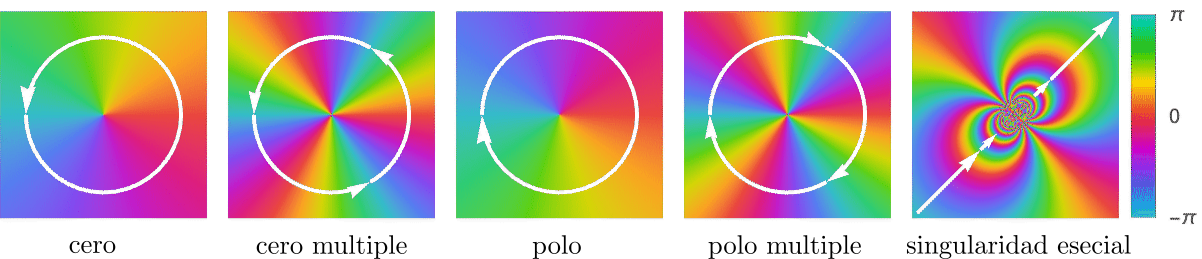
\includegraphics[width=0.75\linewidth]{img/plotco}
	\caption{Ejemplo gráfico del comportamiento de los ceros, polos y singularidades cuando se usa la función ComplexPlot3D}
	\label{fig:plotco}
\end{figure}
\\Y la forma de usar esta función es \textbf{ComplexPlot[$f$,$\{z,z_{min},z_{max}\}$]}, cabe aclarar que esta función genera un grafico de $\mathbf{\operatorname{Arg}[f]}$ sobre el rectángulo en el plano complejo con esquinas $z_{min}$ y $z_{max}$, además que,  la intensidad de los colores esta determinada por el valor absoluto (módulo) de $f$, es decir,  $\mathbf{\operatorname{Abs}[f]}$. El funcionamiento de \textbf{ComplexPlot3D}  es análogo.\\
En la versión 12.1 de \textbf{Mathematica} se introdujo la función \textbf{ComplexContourPlot}, la cual traza los contornos de una función real sobre los complejos. La forma de usar es \textbf{ComplexContourPlot[$f$,$\{z,z_{min},z_{max}\}$]} y además en las posiciones donde $f$ no se evalúa como un número real, se dejan agujeros para que se vea el fondo del gráfico de contorno. La función $f$ generalmente incluirá funciones como Re, Im, Abs y Arg que extraen componentes reales de números complejos para propósitos de comparación.\\\\
\noindent Al lector interesado le sugerimos revisar \cite{Domain_coloring}, allí encontrará una explicación más detallada, sin llegar a ser teórica, acerca de la visualización de funciones complejas usando colores.\\

\begin{defi}
	Sean $f\colon \Omega\to\C$ una función, $a$ un punto interior de $\Omega$ y $r>0$ tal que la cerradura del disco $D(a,r)$ está contenida en $\Omega$. Definimos $A_{f,a,r}\colon[0,2\pi)\to\R$,
	\[
	A_{f,a,r}(\theta) = \operatorname{Arg}(f(a+re^{i\alpha})).
	\]
\end{defi}

\begin{teor}
	Sea $f\colon \Omega\to\C$ una función holomorfa
	y sea $a$ un punto interior del dominio $\Omega$.
	Supongamos que $a$ es un cero de $f$ de orden $m$.
	Entonces, existe $R>0$ tal que para cada $r$ que satisface $0<r<R$,
	la función $A_{f,a,r}$ recorre $m$ veces los valores de $-\pi$ a $\pi$.
\end{teor}

\noindent Usando la función \textbf{Plot3D} de \textbf{Mathematica} podemos visualizar el mapeo como una función de $\R^2 \rightarrow \R$ como sigue
\begin{mmaCell}[functionlocal=y]{Code}
	  Plot3D[x^2 + y^2, {x, -10, 10}, {y, -10, 10}]
\end{mmaCell}

\begin{mmaCell}[moregraphics={moreig={scale=.4}}]{Output}
	\mmaFrac{ \mmaGraphics{1.png}}{}
\end{mmaCell}

Tratando esta función como mapeo de $\C$ a $\C$ y utilizando las funciones \textbf{ComplexPlot} y \textbf{ComplexPlot3D}

\begin{mmaCell}[functionlocal=y]{Code}
	 ComplexPlot[Abs[z]^2, {z, -2 - 2 I, 2 + 2 I}]
\end{mmaCell}

\begin{mmaCell}[moregraphics={moreig={scale=.35}}]{Output}
	\mmaFrac{ \mmaGraphics{1_1.png}}{}
\end{mmaCell}

\begin{mmaCell}{Input}
  ComplexPlot3D[Abs[z]^2, \{z, -2 - 2 I, 2 + 2 I\},\\ColorFunction -> "CyclicLogAbs"]
\end{mmaCell}

\begin{mmaCell}[moregraphics={moreig={scale=.4}}]{Output}
	\mmaFrac{ \mmaGraphics{1_2.png}}{}
\end{mmaCell}
Como podemos ver, al ser $|z|^2$ una función que tiene por codominio los reales, \textbf{Mathematica} la interpreta como un función real al momento de graficarla, y esto último lo podemos comprobar cuando usamos \textbf{ComplexContourPlot}, donde observamos como solo se grafican las curvas de nivel de la componente real y no se gráfica alguna componente compleja.
\begin{mmaCell}{Input}
	 ComplexContourPlot[\{Re[Abs[z]*Abs[z]], Im[Abs[z]*Abs[z]]\},\\\{z, 20\}, PlotLegends -> "Expressions"]
\end{mmaCell}

\begin{mmaCell}[moregraphics={moreig={scale=.35}}]{Output}
	\mmaFrac{ \mmaGraphics{contorno1.png}}{}
\end{mmaCell}


\begin{Ejem}
	Sea $f(z)=z=x+iy$, entonces $u(x,y)=x$ y $v(x,y)=y$. Tenemos
	$$u_x=1=v_y,$$
	$$u_y=0=-v_x.$$
	Como lo anterior se cumple para cualquier $z\in \C$, entonces $f(z)=z$ es complejo diferenciable en todo $\C$.\\
	Usando \textbf{Mathematica}
	\begin{mmaCell}{Input}
		ComplexPlot[z, \{z, -2 - 2 I, 2 + 2 I\}]
	\end{mmaCell}

	\begin{mmaCell}{Input}
		ComplexPlot3D[z, \{z, -2 - 2 I, 2 + 2 I\}]
	\end{mmaCell}

	\begin{mmaCell}{Input}
		ComplexContourPlot[\{Re[z], Im[z]\}, \{z, 2\},\\PlotLegends -> "Expressions"]
	\end{mmaCell}
El código anterior genera las imágenes mostradas en la figura \ref{fig:ej_4}.\\	
	\begin{figure}[htbp!]
		\centering
		\begin{subfigure}{0.25\textwidth}
			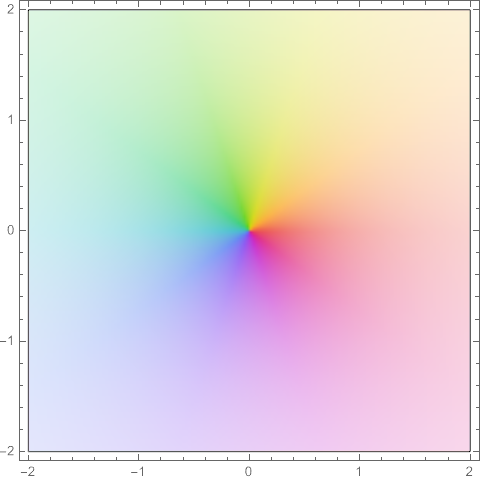
\includegraphics[width=\linewidth]{4_1.png}
			\caption{ComplexPlot.}
			\label{fig:ej_4_1}
		\end{subfigure}
		\begin{subfigure}{0.25\textwidth}
			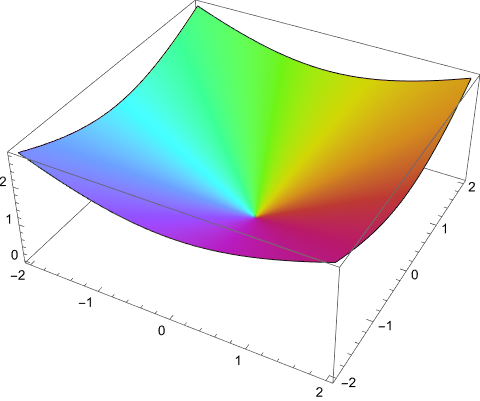
\includegraphics[width=\linewidth]{4_2.png}
			\caption{ComplexPlot3D.}
			\label{fig:ej_4_2}
		\end{subfigure}
		\begin{subfigure}{0.25\textwidth}
			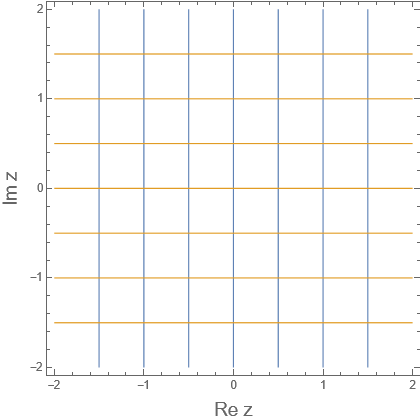
\includegraphics[width=\linewidth]{4_3.png}
			\caption{ComplexContourPlot.}
			\label{fig:ej_4_3}
		\end{subfigure}
		\caption{Diferentes representaciones graficas de la función $f(z)=z$}
		\label{fig:ej_4}
	\end{figure}

\noindent En la figuras \ref{fig:ej_4_1} y \ref{fig:ej_4_2} podemos ver que la función $f(z)=z$ tiene un cero en $z=0$, mientras que en la figura \ref{fig:ej_4_3} vemos que la función identidad no deforma el plano.
\end{Ejem} 


\begin{Ejem}
	Sea $f(z)=\overline{z}=x-iy$, entonces $u(x,y)=x$ y $v(x,y)=-y$. Tenemos
	$$u_x=1,$$
	$$v_y=-1,$$
   entonces $f(z)=\bar{z}$ es no diferenciable en $\C$.\\
	Usando \textbf{Mathematica}
	\begin{mmaCell}{Input}
		ComplexPlot[Conjugate[z], \{z, -2 - 2 I, 2 + 2 I\}]
	\end{mmaCell}
	
	\begin{mmaCell}{Input}
		ComplexPlot3D[Conjugate[z], \{z, -2 - 2 I, 2 + 2 I\}]
	\end{mmaCell}
	
	\begin{mmaCell}{Input}
		ComplexContourPlot[\{Re[Conjugate[z]], Im[Conjugate[z]]\}, \\\{z, 2\},PlotLegends -> "Expressions"]
	\end{mmaCell}
	Obtenemos las figuras mostradas en la figura \ref{fig:ej_4}.\\	
	\begin{figure}[htbp!]
		\centering
		\begin{subfigure}{0.25\textwidth}
			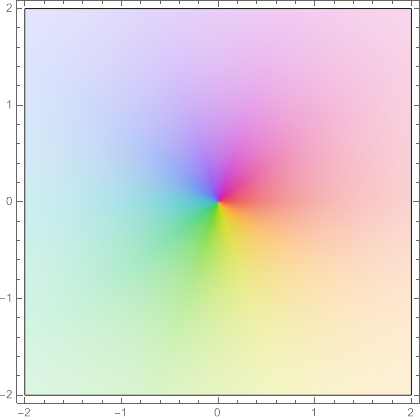
\includegraphics[width=\linewidth]{5_1.png}
			\caption{ComplexPlot.}
			\label{fig:ej_5_1}
		\end{subfigure}
		\begin{subfigure}{0.25\textwidth}
			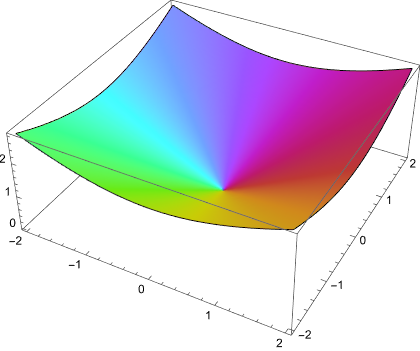
\includegraphics[width=\linewidth]{5_2.png}
			\caption{ComplexPlot3D.}
			\label{fig:ej_5_2}
		\end{subfigure}
		\begin{subfigure}{0.25\textwidth}
			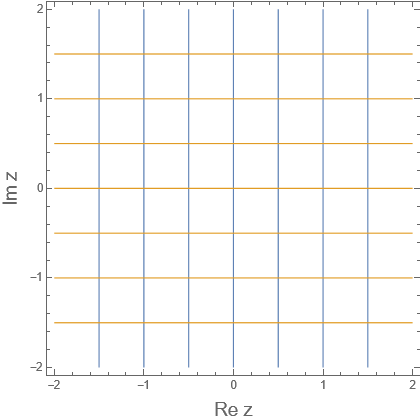
\includegraphics[width=\linewidth]{5_3.png}
			\caption{ComplexContourPlot.}
			\label{fig:ej_5_3}
		\end{subfigure}
		\caption{Diferentes representaciones gráficas de la función $f(z)=\overline{z}$}
		\label{fig:ej_5}
	\end{figure}
	
	En las figuras \ref{fig:ej_5_1} y \ref{fig:ej_5_2} podemos ver que la función $f(z)=\overline{z}$ tiene un cero en $z=0$ y además como reflejan los colores, mientras que en la figura \ref{fig:ej_5_3} vemos que la función tiene un comportamiento similar a la identidad, ya que no deforma el espacio, pero si refleja los puntos.  Para ver esto utilizaremos la función \textbf{ComplexListPlot} para agregar el punto $z=1+i$ y mostrarlo en la gráfica para ver el comportamiento de la función.
	\begin{mmaCell}{Input}
		punto = ComplexListPlot[\{1+1I\},PlotStyle -> Red]\\Show[ComplexContourPlot[\{Re[z], Im[z]\}, \{z, 2\},\\FrameLabel->\{Style["Re z",16],Style["Im z", 16]\}],punto]
	\end{mmaCell}
	
	\begin{mmaCell}{Input}
		punto = ComplexListPlot[\{Conjugate[1+1I]\},PlotStyle->Red]\\Show[ComplexContourPlot[\{Re[Conjugate[z]],Im[Conjugate[z]]\},\\\{z, 2\},FrameLabel -> \{Style["Re z",16], Style["Im z",16]\}],\\punto]
	\end{mmaCell}
	
	Las graficas obtenidas se muestran en la figura \ref{fig:ej_5D}.
	
	\begin{figure}[htbp!]
	\centering
	\begin{subfigure}{0.3\textwidth}
		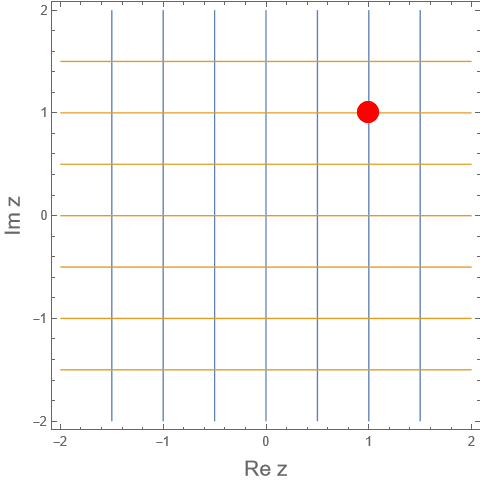
\includegraphics[width=\linewidth]{5_4.png}
		\caption{$f(z)=z$.}
		\label{fig:ej_5_4}
	\end{subfigure}
	\begin{subfigure}{0.3\textwidth}
		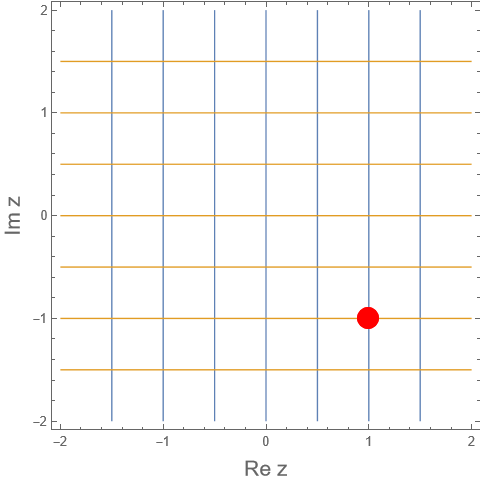
\includegraphics[width=\linewidth]{5_5.png}
		\caption{$f(z)=\overline{z}$.}
		\label{fig:ej_5_5}
	\end{subfigure}
	\caption{Comportamiento discreto de las funciones $f(z)=z$ y $f(z)=\overline{z}$}
	\label{fig:ej_5D}
\end{figure}
\end{Ejem} 



\begin{Ejem}
	Sea 
	\[
		f(z)= \left\{\begin{array}{ccl}
			\dfrac{(z)^5}{|z|^4}, &\mbox{ sí }& z\neq 0\\
			0,&\mbox{ sí }&z=0.
		\end{array} \right. 
		\] 
	 Sí $z=x+iy$, tenemos que $$z^5=x^5+5ix^4y-10x^3y^2-10ix^2y^3+5xy^4+iy^5,$$ así como $$|z|^4=x^4+2 x^2 y^2+y^4.$$
	 Entonces $$u(x,y)=\dfrac{x^5 - 10 x^3 y^2  + 5 x y^4 }{x^4 + 2 x^2 y^2 + y^4},$$  $$v(x,y)=\dfrac{ 5  x^4 y  - 10  x^2 y^3 +  y^5}{x^4 + 2 x^2 y^2 + y^4}.$$
	 Tenemos
	\[
		\begin{array}{c}
			u_x=\dfrac{5 x^4-30 x^2 y^2+5 y^4}{x^4+2 x^2 y^2+y^4}-\dfrac{\left(4 x^3+4 x y^2\right) \left(x^5-10 x^3 y^2+5 x y^4\right)}{\left(x^4+2 x^2 y^2+y^4\right)^2},\\\\
			u_y = \dfrac{20 x y^3-20 x^3 y}{x^4+2 x^2 y^2+y^4}-\dfrac{\left(4 x^2 y+4 y^3\right) \left(x^5-10 x^3 y^2+5 x y^4\right)}{\left(x^4+2 x^2 y^2+y^4\right)^2},\\
			v_x=\dfrac{20 x^3 y-20 x y^3}{x^4+2 x^2 y^2+y^4}-\dfrac{\left(4 x^3+4 x y^2\right) \left(5 x^4 y-10 x^2 y^3+y^5\right)}{\left(x^4+2 x^2 y^2+y^4\right)^2},\\\\
			v_y=\dfrac{5 x^4-30 x^2 y^2+5 y^4}{x^4+2 x^2 y^2+y^4}-\dfrac{\left(4 x^2 y+4 y^3\right) \left(5 x^4 y-10 x^2 y^3+y^5\right)}{\left(x^4+2 x^2 y^2+y^4\right)^2}.
		\end{array}
	\] De lo anterior se desprende que $u(0,0)=v(0,0)=0$, debido a la definición de $f$.\\
	Entonces 
	\[
		\begin{array}{ccl}
			u_x(0,0)&=&\ds\lim_{x\rightarrow 0}\dfrac{u(x,0)-u(0,0)}{x}\\
			&=&\ds\lim_{x\rightarrow 0}\dfrac{x}{x}\\
			&=&1,\\
			v_y(0,0)&=&\ds\lim_{y\rightarrow 0}\dfrac{v(0,y)-v(0,0)}{y}\\
			&=&\ds\lim_{y\rightarrow 0}\dfrac{y}{y}\\
			&=&1,\\
			u_y(0,0)&=&\ds\lim_{y\rightarrow 0}\dfrac{u(0,y)-u(0,0)}{y}\\
			&=&\ds\lim_{x\rightarrow 0}\dfrac{0}{y}\\
			&=&0,\\
		\end{array}
		\]
		\[
		\begin{array}{ccl}
			v_x(0,0)&=&\ds\lim_{x\rightarrow 0}\dfrac{v(x,0)-v(0,0)}{x}\\
			&=&\ds\lim_{x\rightarrow 0}\dfrac{0}{x}\\
			&=&0.
		\end{array}
	\]	
	Luego $f$ satisface las ecuaciones de Cauchy-Riemann en $z=0$.\\
	Por otro lado, tomemos $z=te^{i\theta}$ con $\theta\in \R$ fijo y $t>0$  tal que $t\rightarrow0^{+}$, entonces
	\[
		\begin{array}{ccl}
			f'(z)&=&\ds\lim_{z\rightarrow0}\ds\dfrac{f(z)-f(0)}{z}\\
			&=&\ds\lim_{t\rightarrow0}\dfrac{f(te^{i\theta})}{te^{i\theta}}\\
			&=&\ds\lim_{t\rightarrow0}\dfrac{(te^{i\theta})^5/|te^{i\theta}|^4}{te^{i\theta}}\\
			&=&\ds\lim_{t\rightarrow0}\dfrac{t^5e^{i4\theta}}{t^5}\\
			&=&e^{i4\theta}.
		\end{array}
	\]
	Por otro parte,  $u_x(0,0)+iv_x(0,0)=1$, por lo tanto $f'(0)$ no puede existir. \\
	Usando \textbf{Mathematica}
	\begin{mmaCell}{Input}
		ComplexPlot[(z)^5/((Abs[z])^4), \{z, -2 - 2 I, 2 + 2 I\}]
	\end{mmaCell}
	
	\begin{mmaCell}{Input}
		ComplexPlot3D[(z)^5/((Abs[z])^4), \{z, -2 - 2 I, 2 + 2 I\}]
	\end{mmaCell}
	
	\begin{mmaCell}{Input}
		ComplexContourPlot[\{Re[(z)^5/((Abs[z])^4)],\\Im[(z)^5/((Abs[z])^4)]\}, \{z, 2\},\\PlotLegends -> "Expressions"]
	\end{mmaCell}
	obtenemos las graficas mostradas en la figura \ref{fig:ej_6}.\\	
	\begin{figure}[htbp!]
		\centering
		\begin{subfigure}{0.2\textwidth}
			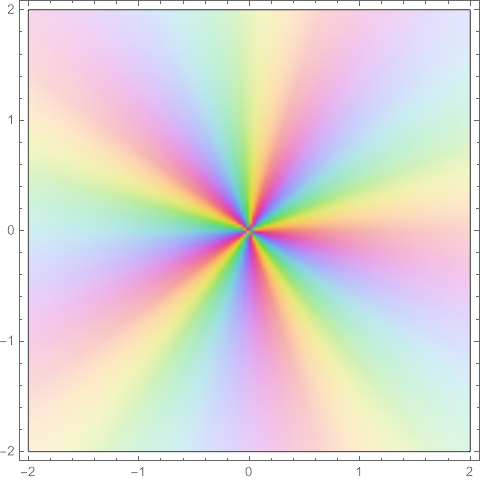
\includegraphics[width=\linewidth]{6_1.png}
			\caption{ComplexPlot.}
			\label{fig:ej_6_1}
		\end{subfigure}
		\begin{subfigure}{0.3\textwidth}
			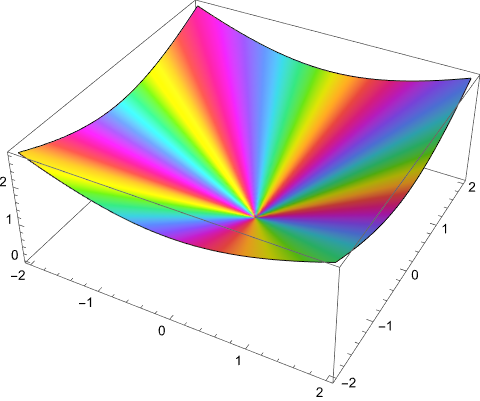
\includegraphics[width=\linewidth]{6_2.png}
			\caption{ComplexPlot3D.}
			\label{fig:ej_6_2}
		\end{subfigure}
		\begin{subfigure}{0.3\textwidth}
			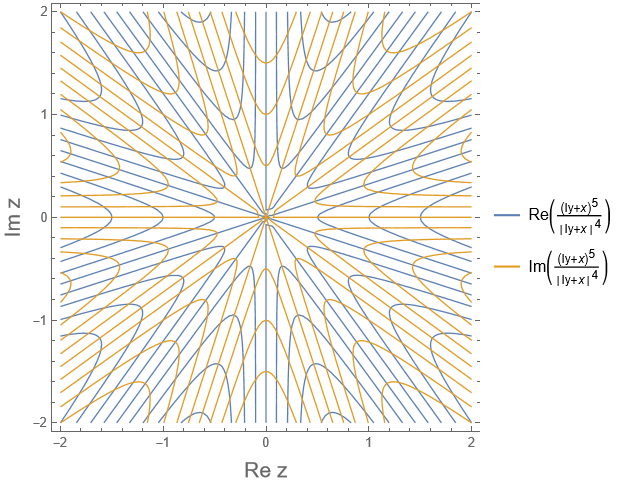
\includegraphics[width=\linewidth]{6_3.png}
			\caption{ComplexContourPlot.}
			\label{fig:ej_6_3}
		\end{subfigure}
		\caption{Diferentes representaciones gráficas de la función $f(z)=\frac{(z)^5}{|z|^4}$}
		\label{fig:ej_6}
	\end{figure}
	
	En las figuras \ref{fig:ej_6_1} y \ref{fig:ej_6_2} podemos ver que la función $f(z)=\frac{(z)^5}{|z|^4}$ tiene un cero de orden 5 en $z=0$, mientras que en la figura \ref{fig:ej_6_3} vemos que la se mapean las componentes reales e imaginarias.
\end{Ejem} 

Hay algunas consecuencias básicas de las ecuaciones de Cauchy-Riemann, las cuales se derivan fácilmente y que tienen consecuencias muy importantes, especialmente en el desarrollo de aplicaciones en matemáticas aplicadas.\\
Considere las curvas $u(x,y)=\mbox{cte}$, $v(x,y)=\mbox{cte}$. El gradiente, $\mbox{grad } u$ es
\[
	\mbox{grad } u=\left(\begin{array}{c}
		\dpartial{u}{x}\\\\
		\dpartial{u}{y}
	\end{array}\right).
\]
Similarmente para $v$. Las ecuaciones de Cauchy-Riemann implican que 
$$\left(\dpartial{u}{x}\right)^2+\left(\dpartial{u}{y}\right)^2=\left(\dpartial{v}{x}\right)^2+\left(\dpartial{v}{x}\right)^2,$$
y $$\dpartial{u}{x}\dpartial{v}{x}+\dpartial{u}{y}\dpartial{v}{y}=0.$$

\begin{teor}\label{Teor8.5silv}
	Si $f(z)$ es analítica en un dominio G, entonces $f(z)$ tiene derivadas de todos los ordenes en $G$, más aun toda derivada $$f^{n}(z)=\dfrac{d^n f(z)}{dz^n},$$ es analítica en $G$ para toda $n=0,1,2,\ldots$.\\
	Una demostración de este teorema puede encontrarla en \cite{silverman}, más precisamente el Teorema 8.5. 
\end{teor}
Ahora, usando el Teorema \ref{Teor8.5silv}, podemos derivar nuevamente y también intercambiar el orden de diferenciación, además de usar las ecuaciones de Cauchy-Riemann para obtener que
$$\dpartial{^2 u}{x^2}=\dfrac{\partial}{\partial x}\left(\dpartial{u}{x}\right)=\dfrac{\partial}{\partial x}\left(\dpartial{v}{x}\right)=\dfrac{\partial}{\partial y}\left(\dpartial{v}{x}\right)=-\dfrac{\partial}{\partial y}\left(\dpartial{u}{y}\right)=-\dpartial{^2u}{y^2},$$
luego
$$\dpartial{^2 u}{x^2}+\dpartial{^2u}{y^2}=0,$$
entonces $u$ satisface la ecuación de Laplace, en este caso diremos que la función es armónica. Similarmente para $v$.

\section{El Teorema de Ahlfors-Struble}
 Sean $z = x + iy$ y $f(z) = u(x, y)+iv(x, y)$. Entonces dada una función $u(x, y)$, a menudo surge la pregunta de cómo encontrar la función $v(x,y)$ correspondiente y, por tanto, el mapeo  $f(z)$. En la mayoría de las veces el problema se soluciona resolviendo las ecuaciones de Cauchy-Riemann. Tenga en cuenta que un paso preliminar y muy sensato es comprobar que $u(x,y)$  satisface la ecuación de Laplace, esto se ilustra en el siguiente ejemplo.
 \begin{Ejem}\label{EjCR}
 	Sea $u(x,y)=x^2-y^2$, encuentre $v(x,y)$ tal que $f(z)=u(x,y)+v(x,y)$ sea complejo diferenciable.
 	\solu
 	\noindent En primer lugar, planteamos nuestro sistema de ecuaciones de Cauchy-Riemann
 	\[
 		\begin{array}{c}
 			\dpartial{u}{x}=\dpartial{v}{y}=2x,\\\\
 			\dpartial{u}{y}=-\dpartial{v}{x}=-2y,
 		\end{array}
 	\]
 	luego integramos las parciales de $v$ y obtenemos
 	\[
 		\begin{array}{c}
 			v(x,y)=2xy+g(x),\\
 			v(x,y)=2yx+h(y),
 		\end{array}
 	\]
 	donde $g,h$ son funciones arbitrarias. Igualando las dos expresiones anteriores, se tiene que $g(x)=h(y)$, es decir, $g$ y $h$ deben de ser constantes. Luego $v=2xy+c$ para alguna constante $c$, por tanto 
 	$$f(z)=x^2-y^2+2ixy+ic=(x+iy)^2+ic=z^2+ic.$$\endproof
 \end{Ejem}
Este ejemplo resulta ser muy sencillo, pero en ocasiones podemos encontrarnos algunos en los cuales la obtención  de $v$ y
por ende de $f$ no son tan sencillos, por ejemplo  la función 
$$u(x,y)=e^{\dfrac{x}{x^2+y^2}}\cos\left(\dfrac{y}{x^2+y^{2}}\right).$$
Este ejemplo lo estudiaremos más adelante utilizando un Teorema que en seguida se enunciara.\\
El Teorema de Ahlfors-Struble nos proporciona un método donde podemos encontrar $f$ a partir de $u$ o a paertir de $v$ de una manera puramente algebraica. El teorema se presenta en dos versiones, la primera de ellas es cuando $f(z)$ es una función complejo diferenciable en una vecindad en el origen y la segunda,  cuando $f(z)$ es una función complejo diferenciable en una vecindad de $a\neq 0$.\\
\noindent Se tiene la siguiente definición
\begin{defi}
	Sea $u:\R^2\rightarrow\R$ una función real, por una extensión natural de $u$ nos referiremos a un función $u_{ex}:\C^2\rightarrow\C$ que se obtiene al sustituir $x,y\in\R$ en $u$ por $w_1,w_2\in\C$.
\end{defi}
\noindent Sean $f(z)$ una función diferenciable en una vecindad en el origen y $\tilde{u}:\C^2\rightarrow\C$ dada por
\begin{equation}\label{AS1}
	\title{u}(w_1,w_2)=\dfrac{1}{2}[f(w_+i_w2)+\hat{f}(w_1-iw_2)],
\end{equation}
en donde  $\hat{f}$ es la reflexión, $\hat{f}:\C\rightarrow\C$ dada por $\hat{f}(z)=\overline{f(\overline{z})}$.\\
\noindent Note que, si  hacemos el cambio de variable 
\begin{equation}\label{AS2}
	w_1=\dfrac{z}{2},\;\;\;w_2=\dfrac{z}{2i},
\end{equation}
donde $z\in\C$, obtenemos 
\begin{equation}\label{AS3}
	\tilde{u}\left(\dfrac{z}{2},\dfrac{z}{2i}\right)=\dfrac{1}{2}[f(z)+\hat{f}(0)]=\dfrac{1}{2}[f(z)+\overline{f(0)}]
\end{equation}
Observemos que si $w_1=x$ y $w_2=y$ con $x,y\in\R$, entonces 
\[
	\begin{array}{ccl}
		\tilde{u}(x,y)&=&\dfrac{1}{2}[f(x+iy)+\hat{f}(x-iy)]\\\\
		&=&\dfrac{1}{2}[f(x+iy)+\overline{f(x+iy)}]\\
		&=&u(x,y),
	\end{array}
\]
ya que para cualquier $z\in\C$ se verifica que $z+\overline{z}=2\operatorname{Re}(z)$. Del análisis anterior, se tiene que $\tilde{u}$ es extensión natural de $\C^2$ de la función real $u(x,y)$. Entonces
\[
	\begin{array}{ccl}
		u\left(\dfrac{z}{2},\dfrac{z}{2i}\right)&=&u_{ex}\left(\dfrac{z}{2},\dfrac{z}{2i}\right)\\\\
		&=&\tilde{u}\left(\dfrac{z}{2},\dfrac{z}{2i}\right)\\\\
		&=&\dfrac{1}{2}[f(z)+\overline{f(0)}]
	\end{array}
\]
El razonamiento anterior, es un esbozo de la demostración del siguiente teorema.

\begin{teor}[Ahlfors-Struble para vecindades en torno al origen]\label{TAS1}
	Sea $f(z)$ diferenciable en una vecindad del origen, con parte real $u(x, y)$ y parte imaginaria $v(x, y)$, donde 
	$z = x + iy$. Entonces, se tiene
	\[
		\begin{array}{ccl}
			f(z)&=&2u\left(\dfrac{z}{2},\dfrac{z}{2i}\right)-\overline{f(0)}\\
			&=&2iv\left(\dfrac{z}{2},\dfrac{z}{2i}\right)+\overline{f(0)},
		\end{array}
	\]
	donde $\overline{f(0)}$ es el conjugado de $f(0)$.
\end{teor}
Consideremos nuevamente el ejemplo \ref{EjCR}, pero ahora lo resolveremos usando el Teorema \ref{TAS1}.
\begin{Ejem}	
	Sea $u(x,y)=x^2-y^2$, encuentre  $f(z)$ usando el Teorema \ref{TAS1}.
	\solu
	\noindent Note que $u(0, 0) = 0$, por lo que $f(0) = i\beta$ para alguna $\beta\in\R$. Aplicando el Teorema \ref{TAS1}
	\[
		\begin{array}{ccl}
			f(z)&=&2u\left(\dfrac{z}{2},\dfrac{z}{2i}\right)-\overline{f(0)}\\
			&=&2\left(\left(\dfrac{z}{2}\right)^2-\left(\dfrac{z}{2i}\right)^2\right)-\overline{f(0)}\\
			&=&2\left(\dfrac{z^2}{4}+\dfrac{z^2}{4}\right)-\overline{i\beta}\\
			&=&z^2+i\beta.
		\end{array}
	\]
	Con  $\beta=0$. 
	\begin{mmaCell}{Input}
		ComplexPlot[z^2, \{z, -2 - 2 I, 2 + 2 I\}]
	\end{mmaCell}
	
	\begin{mmaCell}[moregraphics={moreig={scale=.25}}]{Output}
		\mmaFrac{ \mmaGraphics{8_1.png}}{}
	\end{mmaCell}
 Notemos que en imagen obtenida se tiene que patrón de los colores se repite dos veces alrededor del $0$, esto se debe a que en este punto la función $f(z)=z^2$ tiene un cero de multiplicidad 2.\endproof
\end{Ejem}

\begin{Ejem}	
	Sea $u(x,y)=e^{x} \cos(y)$, encuentre $v(x,y)$ tal que $f(z)=u(x,y)+v(x,y)$ sea complejo diferenciable.
	\solu
	\noindent Vemos que $u(0,0)=1$, luego $f(0)=1+i\beta$ para  alguna $\beta\in\R$. Recordemos que 
	$$\cos p=\dfrac{1}{2}(e^{ip}+e^{-ip}).$$
	Entonces 
	\[
		\begin{array}{ccl}
			f(z)&=&2e^{\frac{z}{2}}\cos\left(\dfrac{2}{2i}\right)-\overline{1+i\beta}\\
			&=&e^{\frac{z}{2}}\left[e^{i\frac{z}{2i}}+e^{-i\frac{z}{2i}} \right]-1+i\beta\\
			&=&e^{z}+i\beta.
		\end{array}
	\]
	Con $\beta=1$
	
	\begin{mmaCell}{Input}
		ComplexPlot[Exp[z] + I,\{z, -10 - 10 I, 10 + 10 I\},\\PlotRange -> Automatic]
	\end{mmaCell}
	
	\begin{mmaCell}[moregraphics={moreig={scale=.25}}]{Output}
		\mmaFrac{ \mmaGraphics{9_1.png}}{}
	\end{mmaCell}
Usando el comando \textbf{Solve} podemos encontrar las soluciones  de la función $f(z)$,
\begin{mmaCell}{Input}
	 Solve[Exp[z] == -I, z]
\end{mmaCell}
de lo anterior obtenemos que las soluciones son $$\left\{z\mid -\dfrac{i\pi}{2} +2 i \pi  k\text{ si }k\in \Z\right\}.$$
Usando un bucle \textbf{For}, obtenemos numéricamente las 3 soluciones que se muestran en la imagen.
\begin{mmaCell}{Input}
	 For[i = -1, i < 2, i++, Print[-0.5*(I*Pi) + 2*I*Pi*i]]
\end{mmaCell}
los cuales resultan ser $-7.85398 i,  -1.5708 i$ y $4.71239i$ para $k=-1,0,1$ respectivamente.\endproof

\end{Ejem}


\begin{teor}[Ahlfors-Struble para vecindades en torno a puntos distintos al origen]\label{TAS2}
	Sea $f(z)$ complejo diferenciable en una vecindad del punto $a$, con parte real $u(x, y)$ y parte imaginaria $v(x, y)$, donde 
	$z = x + iy$. Entonces extendiendo  $u$ (o $v$) a $\C^2$ se tiene
	\[
	\begin{array}{ccl}
		f(z)&=&2u\left(\dfrac{z+\bar{a}}{2},\dfrac{z-\bar{a}}{2i}\right)-\overline{f(a)}\\
		&=&2iv\left(\dfrac{z+\bar{a}}{2},\dfrac{z-\bar{a}}{2i}\right)+\overline{f(a)},
	\end{array}
	\]
	donde $\overline{f(a)}$ es el conjugado de $f(a)$.\\
		La demostración de este teorema se puede consultar en \cite{Shaw-A}, vea el Teorema 2.1.
\end{teor}


\begin{Ejem}[Una función con un polo simple en el origen]
	Sea $u(x,y)=\dfrac{x}{x^2+y^2}$, encuentre $f(z)$.
	\solu Note que 
	$$\left(\dfrac{z+\bar{a}}{2}\right)^{2}+\left(\dfrac{z-\bar{a}}{2i}\right)^2=\dfrac{(z+\overline{a})^2-(z-\overline{a})^2}{4}=\dfrac{4z\overline{a}}{4}=z\overline{a}.$$
	Usando el Teorema \ref{TAS2}
	\[
		\begin{array}{ccl}
			f(z)&=&2u\left(\dfrac{z+\bar{a}}{2},\dfrac{z-\bar{a}}{2i}\right)\\
			&=&2\left(\dfrac{\frac{z+\bar{a}}{2}}{\left(\dfrac{z+\bar{a}}{2}\right)^{2}+\left(\dfrac{z-\bar{a}}{2i}\right)^2}\right)\\
			&=&2\dfrac{z+\bar{a}}{2}\dfrac{1}{z\bar{a}}-\overline{f(a)}\\
			&=&\dfrac{1}{z}+\dfrac{1}{\overline{a}}-\overline{f(a)}.
		\end{array}
	\]
	Vemos que en $z = a$ se tiene la relación $f(a)+\overline{f(a)}=\frac{1}{a}+\frac{1}{\overline{a}}$, es decir, tenemos  que la parte real de $f(a)$ es la parte real de $\frac{1}{\overline{a}}$ , entonces se infiere que
	$$f(z)=\dfrac{1}{z}+i\beta,$$
	con $\beta\in\R$.\\Tomemos $\beta=0$,
	\begin{mmaCell}{Input}
		ComplexPlot[1/z, \{z, -10 - 10 I, 10 + 10 I\},\\PlotRange -> All]
	\end{mmaCell}
	
	\begin{mmaCell}[moregraphics={moreig={scale=.25}}]{Output}
		\mmaFrac{ \mmaGraphics{11_1.png}}{}
	\end{mmaCell}
En la imagen anterior, podemos ver el comportamiento de los colores alrededor del origen. Este comportamiento, es decir, cuando el sentido en el que giran los colores alrededor de un punto se invierte se da cuando la función tiene un polo en dicho punto. \endproof
\end{Ejem}
\begin{teor}[Teorema Grande de Picard]\label{GTP}
	Sea $a$ una singularidad esencial de $f$ en alguna vecindad agujerada. Entonces para cada vecindad agujerada de $a$, $f(z)$ asume todos los números complejos, con una posible excepción, un número infinito de veces.
	La prueba de este teorema se puede consultar en \cite{Conway}, vea el Teorema 4.2.
\end{teor}
\begin{Ejem}[Una función con una singularidad esencial en el origen]
	Sea $$u(x,y)=e^{\dfrac{x}{x^2+y^2}}\cos\left(\dfrac{y}{x^2+y^2}\right),$$  encuentre $f(z)$.
	\solu Tenemos que si $x\rightarrow\frac{z+\overline{a}}{2}$, $y\rightarrow\frac{z-\overline{a}}{2i}$
	\[
		\begin{array}{ccl}
			\dfrac{x}{x^2+y^2}&=&\dfrac{\dfrac{z+\overline{a}}{2}}{\left(\dfrac{z+\overline{a}}{2}\right)^2+\left(\dfrac{z-\overline{a}}{2i}\right)^2}\\
			&=&\dfrac{\dfrac{z+\overline{a}}{2}}{\dfrac{(z+\overline{a})^2-(z-\overline{a})^2}{4}}\\
			&=&\dfrac{\dfrac{z+\overline{a}}{2}}{\dfrac{4\overline{a}z}{4}}\\
			&=&\dfrac{z+\overline{a}}{2z\overline{a}},\\
				\end{array}
			\]
			
			\[
			\begin{array}{ccl}
			\dfrac{y}{x^2+y^2}&=&\dfrac{\dfrac{z-\overline{a}}{2}}{\left(\dfrac{z+\overline{a}}{2}\right)^2+\left(\dfrac{z-\overline{a}}{2i}\right)^2}\\
			&=&\dfrac{\dfrac{z-\overline{a}}{2}}{\dfrac{(z+\overline{a})^2-(z-\overline{a})^2}{4}}\\
			&=&\dfrac{\dfrac{z-\overline{a}}{2}}{\dfrac{4\overline{a}z}{4}}\\
			&=&\dfrac{z-\overline{a}}{2z\overline{a}},
		\end{array}
	\]
	luego
	\[
		\begin{array}{ccl}
			f(z)&=&2\exp\left({\dfrac{z+\overline{a}}{2z\overline{a}}}\right)\cos\left(\dfrac{z-\overline{a}}{2iz\overline{a}}  \right)-\overline{f(a)}\\
			&=&2\exp\left({\dfrac{1}{2\overline{a}}+\dfrac{1}{2z}}\right)\cos\left(\dfrac{1}{2i\overline{a}}-\dfrac{1}{2iz}\right)-\overline{f(a)}\\
			&=&\exp\left({\dfrac{1}{z}}\right)+e^{\dfrac{1}{\overline{a}}}-\overline{f(a)}\\
			&=&\exp\left({\dfrac{1}{z}}\right)+i\beta,
		\end{array}
	\]
	con alguna $\beta\in \R$.\\
	Tomando $\beta=0$,  entonces $f(z)=e^{\frac{1}{z}}$.\begin{mmaCell}{Input}
		ComplexPlot[Exp[1/z], \{z, -1 - 1 I, 1 + 1 I\},\\PlotRange -> Automatic,ColorFunction -> "CyclicLogAbs"]
	\end{mmaCell}
	
	\begin{mmaCell}[moregraphics={moreig={scale=.25}}]{Output}
		\mmaFrac{ \mmaGraphics{11_2.png}}{}
	\end{mmaCell}
La función anterior es bastante interesante, ya que al representarla con colores podemos ver que no hay ningún punto en el cual los colores giren en torno a él, pero justo en el punto $z=0$, vemos como los colores se van alternando infinitamente hasta acercarse  al $0$, este comportamiento de los colores se da cuando se tiene una singularidad esencial.\\
Visualmente lo que podemos ver en la figura, es que la función $e^{\frac{1}{z}}$ toma todos los valores complejos, excepto el $0$, en cualquier vecindad del origen; es decir, esta función satisface el Teorema \ref{GTP}.\endproof
\end{Ejem}


\begin{Ejem}[Una función con un punto de ramificación en el origen]
	Sea $$u(x,y)=\ln(\sqrt{x^2+y^2}),$$  encuentre $f(z)$.
	\solu
	Se tiene que $$u(x,y)=\ln(\sqrt{x^2+y^2})=\dfrac{1}{2}\ln(x^2+y^2),$$
	entonces 
	\[
		\begin{array}{ccl}
			f(z)&=&2\dfrac{1}{2}\ln(z\overline{a})-\overline{f(a)}\\
			&=&\ln(z)+\ln(\overline{a})-\overline{f(a)}\\
			&=&\ln(z)+i\beta,
		\end{array}
	\]
	para alguna $\beta\in \R$.
	Tomando $\beta=0$, entonces $f(z)=e^{\frac{1}{z}}$.
	\begin{mmaCell}{Input}
		ComplexPlot[Log[z], \{z, -2 - 2 I, 2 + 2 I\},\\PlotRange -> Automatic,ColorFunction -> "CyclicLogAbs"]
	\end{mmaCell}
	
	\begin{mmaCell}[moregraphics={moreig={scale=.25}}]{Output}
		\mmaFrac{ \mmaGraphics{12_1.png}}{}
	\end{mmaCell}
\end{Ejem}
Notemos que, en la imagen anterior hay un punto en donde todos los colores se juntan y además la secuencia de colores va en sentido antihorario (azul, rojo, verde), es decir, la función $f(z)$ se anula en dicho punto, el cual resulta ser en el punto $z=1$. Además podemos observar como a la izquierda se juntan algunos colores en una línea  y esto ocurre en torno al cero, podemos ver que el logaritmo presenta ''problemas'' de continuidad, lo anterior está relacionado con las ramas del logaritmo y el punto $z=0$ es un punto de ramificación del logaritmo.\endproof

\subsection{Implementación del algoritmo en Mathematica }
Como expusimos antes, la formula  del Teorema \ref{TAS1} nos permite encontrar $f(z)$ a partir de $u$ o $v$ de forma algebraica. Es por ello que nos proponemos a realizar una implementación del Teorema \ref{TAS1} usando Mathematica, desde luego, utilizaremos esta implementación para realizar una comprobación de los ejemplos presentados anteriormente.\\
\noindent En nuestra implementación usaremos la función \textbf{ComplexExpand} con la opción \textbf{TargetFunctions -> \{Re, Im\}} para obtener la forma correcta de la función en términos de la variable compleja $z$.\\
\noindent Antes de realizar la implementación, expliquemos las funciones mencionadas en el párrafo anterior. En el caso de la función \textbf{ComplexExpand}, nos podemos dar una idea (por el nombre) de lo que realiza esta. Para usar esta función, debemos de pasar por parámetro obligatorio una expresión (\textit{expr}) y opcionalmente una lista de variables $\{x_1,x_2,\ldots,x_n\}$.  Si solo pasamos una expresión \textit{expr}, \textbf{ComplexExpand} solo   expande \textit{expr} asumiendo que todas las variables son reales.En cambio, si le pasamos una lista de variables, \textbf{ComplexExpand} expande \textit{expr} asumiendo que las variables que coinciden con cualquiera de $x_i$ son complejas. SE presentan algunos ejemplos a continuación.

\begin{mmaCell}{Input}
 	 ComplexExpand[Sin[x + I y]]
\end{mmaCell}

\begin{mmaCell}{Output}
	 Cosh[y] Sin[x] + I Cos[x] Sinh[y]
\end{mmaCell}

\begin{mmaCell}{Input}
	 ComplexExpand[Sin[x] Exp[y], {x, y}]
\end{mmaCell}

\begin{mmaCell}{Output}
	 E\^Re[y] Cos[Im[y]] Cosh[Im[x]] Sin[Re[x]] - E\^Re[y] Cos[Re[x]]\\Sin[Im[y]] Sinh[Im[x]] + I (E\^Re[y] Cosh[Im[x]] Sin[Im[y]] \\Sin[Re[x]] + E\^Re[y] Cos[Im[y]] Cos[Re[x]] Sinh[Im[x]])
\end{mmaCell}

La opción \textbf{TargetFunctions -> \{Re, Im\}}, de la función en cuestión, nos da la respuesta en términos de \textbf{Re[z]} y \textbf{Im[z]}

\begin{mmaCell}{Input}
	 ComplexExpand[Tan[z], {z}, TargetFunctions -> {Re, Im}]
\end{mmaCell}

\begin{mmaCell}{Output}
	 \mmaFrac{Sin[2 Re[z]]}{(Cosh[2 Im[z]] + Cos[2 Re[z]])} +\\ \mmaFrac{(I Sinh[2 Im[z]])}{(Cosh[2 Im[z]] + Cos[2 Re[z]])}
\end{mmaCell}
Con lo anterior ya explicado, podemos proceder a la implementación. En esta implementación, desarrollaremos una función que tomara tres parámetros, $expr$, $a$, y una una lista de tres elementos $\{xsym_, ysym_, zsym_ \}$, esta función la llamaremos \textbf{AhlforsStruble1}

\begin{mmaCell}{Input}
	 AhlforsStruble1[expr_, a_, {xsym_, ysym_, zsym_ }] := Module[\\ \{abar = Conjugate[a], exprf\},\\ exprf = ComplexExpand[expr, TargetFunctions -> \{Re, Im\}];\\ func = 2*exprf /. \{xsym -> (zsym + abar)/2, ysym ->\\ (zsym - abar)/(2*I)\};\\ basecorr =  - exprf /. {xsym -> Re[a], ysym -> Im[a]};\\ FullSimplify[func + basecorr + I*\(\pmb{\beta}\)]]
\end{mmaCell}
\noindent Para probar esta función, crearemos una lista de expresiones, estas expresiones serán las funciones  $u$ de los ejemplos anteriores.

\begin{mmaCell}{Input}
	 ConjuntoTestU = \{x^2 - y^2,\\ Exp[x] Cos[y],\\ x/(x^2 + y^2),\\ Exp[x/(x^2 + y^2)] Cos[y/(x^2 + y^2)],\\ Log[Sqrt[x^2 + y^2]]\};
\end{mmaCell}
Usando la función \textbf{Map} de Mathematica y la lista anterior
\begin{mmaCell}{Input}
	  Map[AhlforsStruble1[#, 0.0, {x, y, z}] &, ConjuntoTestU]
\end{mmaCell}
\begin{mmaCell}{Output}
	 \{z^2 + I \(\pmb{\beta}\),\\ E^z + I\(\pmb{\beta}\),\\ Indeterminate,\\ Indeterminate,\\ Indeterminate\}
\end{mmaCell}
\noindent Como podemos ver en el resultado, nuestra implementación arroja un valor indeterminado, esto se debe a que falla cuando el origen no es un punto en el que las funciones estén definidas, sin embargo, si cambiamos el punto $a$, por ejemplo por $a=1$, entonces nuestra implementación funciona sin problemas.

\begin{mmaCell}{Input}
	 Map[AhlforsStruble1[#, 1, {x, y, z}] &, ConjuntoTestU]
\end{mmaCell}
\begin{mmaCell}{Output}
	 \{z^2 + I \(\pmb{\beta}\),\\ E^z + I\(\pmb{\beta}\),\\ 1/z + I \(\pmb{\beta}\),\\ E^(1/z) + I \(\pmb{\beta}\),\\ I \(\pmb{\beta}\) + Log[z]\}
\end{mmaCell}
\noindent Podemos ver que, estos resultados son los mismos que obtuvimos anteriormente.





















 
	
	\chapter{Mapeos conformes} \label{chap:background}
\section{Introducción}\label{introcap2}
\begin{defi}
	Sean $\Omega_{1}$ y $\Omega_{2}$ dos conjuntos abiertos. Un mapeo analítico e inyectivo $f:\Omega_{1}\rightarrow\Omega_{2}$  es llamado un homeomorfismo analítico de  $\Omega_{1}$ sobre $\Omega_{2}$. Un mapeo analítico e inyectivo de $\Omega_{1}$ a $\Omega_{2}$ es llamado un mapeo conforme de $\Omega_{1}$ a $\Omega_{2}$.\\
	Diremos que $\Omega_{1}$ y $\Omega_{2}$ son conformemente equivalentes si existe un mapeo conforme de $\Omega_{1}$ a $\Omega_{2}$ y cuyo rango sea $\Omega_{2}$, en ese caso escribiremos $\Omega_{1} \sim\Omega_{2}$.
\end{defi}
\begin{defi}
	Diremos que la curva $l$ parametrizada por $\lambda$ en $[a,b]$ y diferenciable en $t_0$ tiene tangente $\tau$ en $\lambda(t_0) = z_0$ si existe el límite $\theta = \ds\lim_{t\rightarrow t0}\mbox{Arg}r(t)$  donde
	$$r(t)=\dfrac{\lambda(t)-\lambda(t_0)}{t-t_0},$$ entonces se dirá que $l$ tienen tangente con inclinación $\theta$
\end{defi}

\begin{teor}
	Sean $G$ un dominio y $f$ continua en $G$ supongamos que $f(z)$ tiene derivada
	distinta de cero en $z_0 \in G$ y que $l$ es una curva que pasa por $z_0$ y que tiene tangente $\tau$ en
	$z_0$. Entonces $w = f(z)$ mapea $l$ en una curva $L$ en el plano $w$ que pasa por $w_0 = f(z_0)$ y con
	tangente $T$ en $w_0$ además la inclinación de $T$ excede a $\tau$ en $\mbox{Arg}'f(z_0)$.\\
	Para consultar la demostración le sugerimos ver el Teorema 3.3 de \cite{silverman}.
\end{teor}

\begin{teor}
	Sea $G$ un dominio y $f$ analítica en $G$. Entonces $f$ es un mapeo conforme de primer
	tipo en todo punto donde $f'(z) \neq 0$.
\end{teor}

\noindent A partir del teorema anterior se deduce el siguiente corolario.

\begin{coro}
	Supongamos que $l_1$ y $l_2$ son curvas que se cruzan en $z_0\in G$ y que $l_1$ tiene tangente $\tau_1$ y $l_2$ tiene tangente $\tau_2$ en $z_0$. Supongamos que $f$ es diferenciable en $z_0$ con $f^{'}_0(z_0)\neq 0$. Entonces bajo $f$, $l_1$ va a dar a una curva $L_1$ y $l_2$ a una curva $L_2$ que por el teorema pasarán por $w_0 = f(z_0)$ con respectivas tangentes $T_1$ y $T_2$ en $w_0$.
\end{coro}
De lo anterior podemos concluir que $(|f'(z_0)|,\mbox{Arg}f(z_0))$ nos da una descripción de como deforma $f$ al dominio en $z_0$.\\
Nuestro primer objetivo es usar Mathematica para explorar algunos mapeos simples. Lo haremos cargando el paquete \textbf{ParametricPlot}, este paquete contiene dos funcionalidades las cuales son  \textbf{CartesianMap} y \textbf{PolarMap} las cuales nos permiten hacer gráficos utilizando coordenadas cartesianas y polares respectivamente. \\
A manera de ejemplo y para mostrar el uso de estas dos funcionalidades, primero consideraremos la función $f(z)=e^{z}$ en la región $$A=\{z=x+iy\in\C | -1\leq x\leq 1, \; -2\leq y\leq 2\}.$$

\begin{mmaCell}{Input}
	 ParametricPlot[Through[{Re, Im}[Exp[x + I*y]]], \{x,-1,1\},\\\{y,-2,2\},  PlotStyle -> None, Mesh -> 15];
\end{mmaCell}


\begin{mmaCell}[moregraphics={moreig={scale=0.4}}]{Output}
	\mmaFrac{ \mmaGraphics{5.png}}{}
\end{mmaCell}
En el código anterior usamos la función \textbf{Through} de Mathematica, esta función distribuye los operadores que aparecen dentro de los encabezados de las expresiones, por ejemplo podemos usar esta función para aplicar a una lista de funciones un mismo argumento, que fue lo que realizamos en el anterior código.
\begin{mmaCell}{Input}
	 Through[\{f, g, h\}[x]];
\end{mmaCell}
\begin{mmaCell}{Output}
	 \{f[x],g[x],h[x]\}
\end{mmaCell}
Ahora consideremos la función $f(r,t)=\sqrt{re^{it}}$ en la región
$$A=\{(r,t)| 0\leq r\leq t,\; 0\leq t\leq 2\pi \}.$$

\begin{mmaCell}{Input}
	 ParametricPlot[Through[{Re, Im}[Sqrt[r Exp[I t]]]],\{r,0,1\},\\\{t,0, 2Pi\},PlotStyle -> None, Mesh -> 15]
\end{mmaCell}

\begin{mmaCell}[moregraphics={moreig={scale=0.4}}]{Output}
	\mmaFrac{ \mmaGraphics{6.png}}{}
\end{mmaCell}
En \textbf{Mathematica 12.1} se introdujo la función \textbf{ComplexRegionPlot}, para usar esta función basta escribir  ComplexRegionPlot[$pred$,{$z$,$z_{min}$,$z_{max}$}] y se generará un gráfico que muestra la región en el plano complejo para el cual el parámetro  \emph{pred} es Verdadero. Por otro lado si lo que requerimos es graficar regiones dadas por múltiples predicados $pred_i$ escribiremos  ComplexRegionPlot[{$pred_1,pred_2$,$\ldots$},{$z$,$z_{min}$,$z_{max}$}] y donde el predicado, $pred_i$, puede ser cualquier combinación lógica de desigualdades. El $pred_i$ generalmente involucrará funciones como Re, Im, Abs y Arg que extraen componentes reales de números complejos para propósitos de comparación. \\
Teniendo esto en cuenta para graficar la región $\Omega=\left\{z\in\C |\dfrac{1}{2}\leq |z|\leq 1\right\}$  se haría de la siguiente manera:
\begin{mmaCell}{Input}
	 ComplexRegionPlot[1/2 <= Abs[z] <= 1, \{z, -1 - I, 1 + I\}]
\end{mmaCell}

\begin{mmaCell}[moregraphics={moreig={scale=0.4}}]{Output}
	\mmaFrac{ \mmaGraphics{7.png}}{}
\end{mmaCell}

Y para graficar varias regiones, por ejemplo $\Omega=\{z\in \C | \mbox{Re}(z^2)\leq 2 \wedge \mbox{Im}(z^2)>1\}$ 
\begin{mmaCell}{Input}
    ComplexRegionPlot[Re[z^2] <= 2 && Im[z^2] > 1,\\\{z, -10 - 10 I, 10 + 10 I\}]
\end{mmaCell}

\begin{mmaCell}[moregraphics={moreig={scale=0.4}}]{Output}
	\mmaFrac{ \mmaGraphics{8.png}}{}
\end{mmaCell}


Ahora extendemos la funcionalidad del paquete \textbf{ParametricPlot} definiendo un par de funciones que nos muestran cómo se deforma el plano mediante un mapeo conforme  mediante mapeos polares y cartesianos.\\
\begin{mmaCell}{Input}
	 polarMap[func_, radial_, polar_, options___] := \\ ParametricPlot[Evaluate[Through[\{Re, Im\}[func]]],\\ radial, polar,options]
\end{mmaCell}

\begin{mmaCell}{Input}
  cartesianMap[func_, xrange_, yrange_, options___] := \\ParametricPlot[Evaluate[Through[\{Re, Im\}[func]]],\\ xrange, yrange, options]
\end{mmaCell}

A partir de estas funciones reconstruiremos dos más que nos permitirán ver como se ve el plano tanto antes como después de aplicar un mapeo conforme
\begin{mmaCell}{Input}
	 polarConformal[func_, radial_, polar_, options___] :=\\Show[GraphicsGrid[\{\{polarMap[rExp[I t],\\radial, polar, options, DisplayFunction ->Identity,\\PlotRange -> All],polarMap[func, radial, polar, options,\\DisplayFunction ->Identity,\\PlotRange -> \{\{-d, d\}, \{-d, d\}\}]\}\}],\\DisplayFunction -> \$DisplayFunction]
\end{mmaCell}
en la función el valor $d$ representa que tan grande se va a construir el plano.
\begin{mmaCell}{Input}
	 cartesianConformal[func_, xrange_, yrange_, options___] :=\\Show[GraphicsGrid[\{\{cartesianMap[x + I*y, xrange, yrange,\\options,DisplayFunction -> Identity],\\cartesianMap[W[x + I*y],xrange, yrange, options,\\DisplayFunction -> Identity]\}\}],\\DisplayFunction -> \$DisplayFunction]
\end{mmaCell}


\section{Algunos mapeos sencillos y su visualización} \label{mum}
El propósito de esta sección es mostrar el uso de las funciones \textbf{cartesianConformal} y \textbf{polarConformal} cuando se utilizan por parámetros funciones sencillas y ver que les sucede a las regiones en el plano complejo cuando son mapeadas bajo estas funciones. 
\subsection{La función $f(z)=z^n$}

Consideremos dos números complejos $z_1$ y $z_2$ arbitrarios, los podemos escribir en forma trigonométrica
\[
	\begin{array}{c}
		z_1=r_1(\cos\Phi_1+i\sin\Phi_1),\\
		z_2=r_2(\cos\Phi_2+i\sin\Phi_2),
	\end{array}
\]
donde 
\[
	\begin{array}{ccl}
		r_1=|z_1|,&&\Phi_1=\mbox{Arg}z_1,\\
		r_2=|z_2|,&&\Phi_2=\mbox{Arg}z_2,
	\end{array}
\]
entonces 
\[
	\begin{array}{ccl}
		z_1z_2&=&r_1r_2[(\cos\Phi_1\cos\Phi_2-\sin\Phi_1\sin\Phi_2)+i(\sin\Phi_1\cos\Phi_2+\cos\Phi_1\sin\Phi_2)]\\
		&=&r_1r_2[\cos(\Phi_1+\Phi_2)+i\sin(\Phi_1+\Phi_2)],
	\end{array}
\]
por tanto
\[
\begin{array}{c}
	|z_1z_2|=|z_1||z_2|,\\
	\mbox{Arg}z_1z_2=\mbox{Arg}z_1+\mbox{Arg}z_2,
\end{array}
\]
Si $z_1=z_2=z=r(\cos\Phi+i\sin\Phi)$, entonces
$$z^2=r^2[\cos(2\Phi)+i\sin(2\Phi)],$$ 
por inducción se demuestra que para $n\geq 1$ se verifica que 
$$z^n=r^n[\cos(n\Phi)+i\sin(n\Phi)].$$
Cuando $r=1$, obtenemos la fórmula de De Moivre
$$z^n=\cos(n\Phi)+i\sin(n\Phi).$$
así, cuando aplicamos la función $f(z)=z^n$ aplicada el cuarto de círculo $$Q=\left\{z\in \C | |z|=1\; 0\leq \Phi\leq \dfrac{\pi}{2}\right\},$$
lo que obtendremos será como se ''multiplica'' este conjunto $n$ veces, por ejemplo para $n=2$ tenemos el siguiente conjunto
$$Q_1=\{z\in \C | |z|=1,\; 0\leq \Phi\leq \pi\}.$$
\begin{Ejem}
	Sea $f(z)=z^{n}$. En \textbf{Mathematica} podemos visualizar él comportamiento de esta función aplicada al conjunto $Q$, por simplicidad y  solo para ilustrar se tomarán los casos cuando $n=2,3$ y $n=4$.\\
Para $n=2$, si $f_1(z)=z^2$ tenemos
\begin{mmaCell}{Input}
	 f1[z_] = z^2 \\polarConformal[f1[r Exp[I t]], \{r, 0, 1\}, \{t, 0, Pi/2\},\\Mesh -> \{30, 30\}, PlotRange -> All,\\LabelStyle -> Directive[Larger, Bold], PlotStyle -> White,\\MeshStyle -> Blue, Axes -> True]
\end{mmaCell}
\begin{mmaCell}[moregraphics={moreig={scale=0.7}}]{Output}
	\mmaFrac{ \mmaGraphics{17.png}}{}
\end{mmaCell}
Para $n=3$, si $f_2(z)=z^3$, entonces  tenemos el siguiente comportamiento
\begin{mmaCell}{Input}
	 f2[z_] = z^3 \\polarConformal[f2[r Exp[I t]], \{r, 0, 1\}, \{t, 0, Pi/2\},\\Mesh -> \{30, 30\}, PlotRange -> All,\\LabelStyle -> Directive[Larger, Bold], PlotStyle -> White,\\MeshStyle -> Blue, Axes -> True]
\end{mmaCell}
\begin{mmaCell}[moregraphics={moreig={scale=0.7}}]{Output}
	\mmaFrac{ \mmaGraphics{18.png}}{}
\end{mmaCell}
Y para $n=4$, con $f_3(z)=z^4$, se tiene 
\begin{mmaCell}{Input}
	 f3[z_] = z^4 \\polarConformal[f3[r Exp[I t]], \{r, 0, 1\}, \{t, 0, Pi/2\},\\Mesh -> \{30, 30\}, PlotRange -> All,\\LabelStyle -> Directive[Larger, Bold], PlotStyle -> White,\\MeshStyle -> Blue, Axes -> True]
\end{mmaCell}
\begin{mmaCell}[moregraphics={moreig={scale=0.7}}]{Output}
	\mmaFrac{ \mmaGraphics{19.png}}{}
\end{mmaCell}

\end{Ejem}

Como podemos ver en el ejemplo anterior, el efecto del mapeo $z^n$ sobre un punto arbitrario este sera mapeado con  $n$ veces su argumento ya que
$$\mbox{Arg}z_1z_2\cdots  z_n=\mbox{Arg}z_1+\mbox{Arg}z_2+\cdots+\mbox{Arg}z_n,$$
luego, $$\mbox{Arg}z^n=n\mbox{Arg}z$$

\subsection{La función $f(z)=z^\frac{n}{m}$, $m\neq 0$}
Consideremos $n=1$ y $m>0$, y $z=r(\cos\Phi+i\sin\Phi)$, entonces usando la fórmula de De Moivre se obtiene
$$z^\frac{1}{m}=\sqrt[m]{|z|}\left(\cos\dfrac{\mbox{Arg}z}{m}+i\sin\dfrac{\mbox{Arg}z}{m}\right),$$
donde $\mbox{Arg}z=\frac{\theta+2\pi k}{n}$ y $k=0,1,\ldots,m-1$.\\
Si $n>1$, nuevamente usando la fórmula de De Moivre se obtiene
$$z^\frac{n}{m}=|z|^{\frac{n}{m}}\left(\cos\dfrac{n\mbox{Arg}z}{m}\right)+i\sin\dfrac{n\mbox{Arg}z}{m}.$$
Al tomar potencias fraccionarias adecuadas, el efecto de un mapeo de la forma $f(z)=z^n$ se puede deshacer. Por ejemplo, el mapeo $g(z)=z^\frac{1}{2}$ revierte el efecto hecho a una región por el mapeo $f(z)=z^2$, como lo podemos ver a continuación
\begin{mmaCell}{Input}
 	f5[z_] = z^(1/2) \\polarConformal[f5[r Exp[I t]], \{r, 0, 1\}, \{t, 0, Pi\},\\Mesh -> \{30, 30\}, PlotRange -> All,\\LabelStyle -> Directive[Larger, Bold], PlotStyle -> White,\\MeshStyle -> Blue, Axes -> True]
\end{mmaCell}
\begin{mmaCell}[moregraphics={moreig={scale=0.7}}]{Output}
	\mmaFrac{ \mmaGraphics{21.png}}{}
\end{mmaCell}

\subsection{La función $f(z)=e^z$}
Una función entera que no es un polinomio se llama función entera.
trascendental. El ejemplo más simple de este tipo  funciones es la
función exponencial  $e^z$, obtenida extendiendo adecuadamente la
función de variable real $e^x$, donde $x\in\R$, al caso donde $x$ toma
valores complejos arbitrarios, es decir, se reemplaza $x$ por la variable compleja $z = x + iy$. Se tiene el siguiente teorema que caracteriza a la función exponencial
\begin{teor}
	Hay una  única función $f(z) = e^z$ con las siguientes propiedades
	\begin{itemize}
		\item [1.] $f(z)$ está definida y tiene un solo valor para todo complejo (finito) $z$, toma  valores reales cuando $z$ es real, y en particular toma el valor $e$ cuando $z = 1$;
		\item [2.] $f(z)$  satisface el teorema de la suma
		$$f(z_1+z_2)=f(z_1)f(z_2),$$
		\item [3.] $f(z)$ es complejo diferenciable para todo $z$, es decir, $f(z)$ es entera.
	\end{itemize}
\proof Vea el Teorema 6.1 de \cite{silverman}.\endproof 
\end{teor}
Aplicando estas tres propiedades se demuestra que 
$$f(z)=e^z=e^x(\cos x+i\sin y).$$
Se sigue qué $e^z\neq 0$ para todo $z$ y 
\[
	 \begin{array}{ccl}
	 	|e^z|=e^x,&&\mbox{Arg}e^zy+2\pi k.
	 \end{array}
\]
Para $z=iy$ obtenemos la fórmula de Euler
$$e^{iy}\cos y+i \sin y.$$
Usando la ecuación anterior, podemos reemplazar la forma trigonométrica de un número complejo
$$z=r(\cos\Phi+i\sin\Phi),$$
por la forma polar
$$z=re^{i\Phi}.$$
Es claro que la exponencial es periódica en $z$ con periodo $2\pi i$. En otras palabras, si $z$ cambia por $2\pi i$, entonces $y$ cambia por $2\pi$, el valor de $e^z$ no cambia
$$e^{z+2\pi i}=e^z.$$
Consideremos $\omega$ otro periodo de $e^z$, con $\omega=\alpha+i\beta$, entonces 
$$e^{z+\omega}=e^z.$$
para $z$ arbitrario, en particular tenemos
$$e^\omega=e^{\alpha+i\beta}=e^{\alpha}(\cos\beta+i\sin\beta)=1,$$
para $z=0$.  Esto significa que $|e^{\omega}|=e^\alpha=1$, lo cual implica que $\alpha=0$, por lo tanto $\cos\beta+i\sin\beta=1$, es decir, $\beta=2k\pi i$, de modo que 
$$\omega=\alpha+i\beta=2k\pi i,$$
lo anterior muestra que $2\pi i$ es el período fundamental (o primitivo) de la función $e^z$, es decir, que cualquier otro período $\omega$ de $e^z$ debe ser de la forma $2k\pi i$.\\
La expresión $e^{\infty}$ se considerará sin sentido, ya que
$$\lim_{z\to \infty}e^z,$$
no existe. Esto se puede ver por el hecho de que $e^x \to \infty$ cuando $x \to +\infty$,
mientras que $e^x \to 0 $ cuando $x \to -\infty$. En particular, se sigue que $e^z$ no puede coincidir con algún polinomio, es decir, $e^z$ es en realidad una función trascendental entera, ya que cualquier polinomio (excluyendo el caso trivial de una constante) tiende a infinito cuando $z \to \infty$.\\
Ahora nos proponemos a estudiar el comportamiento geométrico del mapeo $w=e^z$. Como ya habíamos dicho antes $e^z\neq0$ para todo $z$, esto significa que el origen de coordenadas en el plano $W$ no pertenece a la imagen del plano $Z$ bajo el mapeo $w=e^z$, sin embargo, cualquier otro punto  del plano $W$ si pertenece a la imagen. De hecho, de la ecuación $w=e^z$, donde $w\neq0$ y $z=x+iy$ es una variable desconocida, obtenemos 
\[
	\begin{array}{ccl}
		|w|=e^x&\mbox{o}&x=\ln |w|,
	\end{array}
\]
y 
\[
\begin{array}{ccl}
	\mbox{Arg}w=y+2k\pi&\mbox{o}&y=\mbox{Arg }w,
\end{array}
\]
Por tanto las preimágenes del punto $w$ sólo pueden ser de la forma
$$z=\ln|w|+i\mbox{Arg}w,$$
Claramente hay infinidad de puntos que satisfacen la ecuación anterior, ya que $\mbox{Arg} w $ toma infinitos valores, todos  múltiplos enteros de $2\pi$. Además, cada uno de estos puntos es en realidad  imagen inversa de $w$, ya que
\[
\begin{array}{ccl}
	\exp[\ln|w|+i\mbox{Arg }w]&=&e^{\ln|w|}(\cos\mbox{Arg }w+i\sin\mbox{Arg }w)\\
	&=&|w|(\cos\mbox{Arg }w+i\sin\mbox{Arg }w)\\
	&=&w.
\end{array}
\]
Por lo tanto, el conjunto de todas las raíces de la ecuación $e^z=w$ ($w\neq 0$) es dado por la ecuación 
$$z=\ln|w|i\mbox{Arg }w=\ln|w|+i(\mbox{arg }w+2\pi k,$$
donde $k\in\Z$. Todos estos puntos se encuentran en la misma línea recta paralelas al eje imaginario  y la distancia entre cualesquiera dos de estos puntos consecutivos  es $2\pi$. Por lo tanto la función $w=e^z$ mapea el plano $Z$ en el plano $W$ sin el origen $w=0$, pero este mapeo no es inyectivo, pues todo punto $w\neq0$ tiene un número infinito de preimágenes. Por otro lado, este mapeo es conforme en cada punto del plano $Z$, $z\neq\infty$, pues 
$$(e^z)'=\dpartial{(e^x\cos y)}{x}+i \dpartial{(e^x\sin y)}{x}=e^{x}(\cos y+i\sin y)=e^z,$$
no se anula para ningún valor de $z$.\\
Supongamos que $z$ traza una línea recta paralela a uno de los ejes coordenados. Por ejemplo, consideremos la línea
$$z=b+it,$$
paralela al eje imaginario. Entonces la imagen de esta expresión bajo es mapeo $w=e^z$ es la curva
$$w=e^b(\cos t+i\sin t),$$ 
es decir, $w$ traza una circunferencia de radio $e^b$ con centro en el origen. Además, como $z$ describe la línea $z=b+it$ de tal manera que $t$, la ordenada de $z$, incrementa continuamente de $-\infty$ a $\infty$, $w$ describe el círculo dado por la expresión  $w=e^b(\cos t+i\sin t)$ y número infinito de veces en la dirección positiva (en sentido antihorario). Por ejemplo, consideremos la línea
\[
	\begin{array}{c}
		z=\dfrac{1}{2}+it,
	\end{array}
\]
entonces de acuerdo con lo anterior la imagen de esta línea bajo el mapeo $w=e^z$ es la curva
$$w=e^{1/2}(\cos t+i\sin t),$$
es decir, la imagen es un círculo con centro en el origen y de radio $e^{\frac{1}{2}}\approx1.64872$
Veamos esto último en Matemática 
\begin{mmaCell}{Input}
	 f[z_] = Exp[z] \\cartesianConformal[f[(x + I*y)], \{x, 0, 1\}, \{y, -2Pi, 2Pi\},\\Mesh -> 1,LabelStyle -> Directive[Larger, Bold],\\PlotStyle -> White,MeshStyle -> Red, Axes -> True,\\PlotPoints -> 40]
\end{mmaCell}
\begin{mmaCell}[moregraphics={moreig={scale=0.5}}]{Output}
	\mmaFrac{ \mmaGraphics{expz.png}}{}
\end{mmaCell}
Ahora consideremos la línea 
$$z=t+ic,$$
paralela al eje real, entonces la imagen de esta línea bajo el mapeo $w=e^z$ es la curva
$$w=e^t(\cos c+i\sin c),$$
es decir, $w$ traza un rayo de pendiente $\tan c$ que emana del origen. Además, como $z$ describe la línea $z=t+ic$ de tal manera que $t$, la abscisa de $z$,  incrementa continuamente de $-\infty$ a $\infty$, $w$ describe el rayo $w=e^t(\cos c+i\sin c)$ de tal manera que la distancia de $w$ desde el origen aumenta continuamente
de $0$ a $\infty$ (por supuesto, los límites $0$ y $\infty$ están excluidos, puesto que $|w|=e^t$. Consideremos las líneas 
$$z=t+i,$$
 entonces la imagen de esta línea bajo el mapeo $w=e^z$ es el rayo que emana del origen descrito por la curva
$$w=e^t(\cos(1)+i\sin(1)),$$ 
en Mathematica 
\begin{mmaCell}{Input}
	 f[z_] = Exp[z] \\cartesianConformal[f[(x + I*y)], \{x, -10, 10\}, {y, 0, 2 Pi},\\Mesh -> \{\{0\}, \{1\}\}, LabelStyle -> Directive[Larger, Bold],\\PlotStyle -> White, MeshStyle -> Red, Axes -> True,\\PlotPoints -> 40]
\end{mmaCell}
\begin{mmaCell}[moregraphics={moreig={scale=0.5}}]{Output}
	\mmaFrac{ \mmaGraphics{expz1.png}}{}
\end{mmaCell}
Así, bajo el mapeo $w = e^z$, una familia de rectas paralelas al eje imaginario se transforma en una familia de círculos concéntricos con centro en el origen, y una familia de rectas paralelas al eje real se transforma en una familia de rayos que emanan del origen.\\
Consideremos el $G$ que consiste en todos los puntos  $z$ tales que 
$$\phi_1<\mbox{Im }z<\phi_2,$$
donde $\phi_2-\phi_1=h$, tal dominio es llamado la banda  abierta de ancho $h$. Supongamos que $0<h<2\pi$, y sea $G_1$ la imagen de $G$ bajo el mapeo $w=e^z$. Se sigue que $G_1$ es el interior del ángulo de $h$ radianes con vértice en el origen formado por los rayos
\[
	\begin{array}{ccccc}
		\mbox{Arg }w=\phi_1+2\pi k,&&\mbox{Arg }w=\phi_2+2\pi k&&(k\in \Z).
	\end{array}
\]
Además, la correspondencia entre los dominios $G$ y $G_1$ bajo el mapeo $w=e^z$ es inyectiva.\\
Por lo tanto, la función $w=e^z$ es un mapeo conforme uno a uno de la franja abierta con ancho $h\leq 2\pi$ con lados paralelos al eje real en el interior de un ángulo de $h$ radianes con vértice en el origen.

\begin{Ejem}
	Esto lo podemos comprobar usando Mathematica, consideremos $\phi_1=\dfrac{\pi}{2}$ y $\phi_2=\pi$, entonces $h=\dfrac{\pi}{2}$, es decir vamos a ver el comportamiento de la banda con ancho $h=\dfrac{\pi}{2}$.
	\begin{mmaCell}{Input}
		f[z_] = Exp[z] \\f[(x + I*y)], {x, -10, 10}, {y, Pi/2, Pi},\\Mesh -> 100, LabelStyle -> Directive[Larger, Bold],\\PlotStyle -> White, MeshStyle -> Red, Axes -> True,\\PlotPoints -> 40]
	\end{mmaCell}
	
	\begin{mmaCell}[moregraphics={moreig={scale=0.5}}]{Output}
		\mmaFrac{ \mmaGraphics{expz2.png}}{}
	\end{mmaCell}
\end{Ejem}

\begin{Ejem}
	

Consideremos la función $f(z)=e^z$ y la región $$\Omega_{1}=\{z\in \C \mid \mbox{Re}(z)\in [0,1]\;, \mbox{Im}(z)\in [0,2\pi]\}.$$
Usando la función \textbf{cartesianConformal} vemos que la imagen de $\Omega_{1}$ bajo $f_1$ resulta ser un anillo que se muestra a continuación
\begin{mmaCell}{Input}
	 f[z_] = Exp[z] \\cartesianConformal[f[(x + I*y)], \{x, 0, 1\}, \{y, -Pi, Pi\},\\Mesh -> 50,LabelStyle -> Directive[Larger, Bold],\\PlotStyle -> White,MeshStyle -> Blue, Axes -> True,\\PlotPoints -> 40]
\end{mmaCell}
\begin{mmaCell}[moregraphics={moreig={scale=0.5}}]{Output}
	\mmaFrac{ \mmaGraphics{22.png}}{}
\end{mmaCell}
es decir la región 
$$\Omega_{2}=\{z\in \C\mid 1<|z|<e\}.$$
\end{Ejem}


%% función logaritmo
\subsection{La función $f(z)=\ln z$}
La inversa de la función $z=e^w=e^{u}(\cos v +i\sin v)$
es definida para cualquier valor diferente de $0$ y $\infty$, y se expresa por la fórmula 
$$w=\ln|z|+i\mbox{Arg}z.$$
Esta función, que es multivaluada, es llamada el logaritmo y es denotado por $\mbox{Ln}z$, es decir, 
$$\mbox{Ln}z=\ln|z|+i\mbox{Arg}z.$$
El valor $$\ln|z|+i\mbox{arg}z,$$ es llamado el valor principal y es denotado por $\ln\;z$. Entonces la expresión para $\mbox{Ln}z$ se puede reescribir como
$$\mbox{Ln}z=\ln z+2k\pi i,$$
donde $k\in\Z$. Se sigue que para cada número complejo, diferente de cero y del infinito, posee un conjunto infinito de logaritmos (es decir, de valores de la función logarítmica); dos valores cualesquiera de éstos de diferencian en un entero múltiplo de $2\pi i$. Si $z\in \R^{+}$, el valor principal del logaritmo coincide con $\ln|z|$, y por consiguiente es aquel número real cuando considerábamos el logaritmo como una función de variable real.\\
Pero, además de estos valores reales, los logaritmos de los números positivos poseen también un conjunto infinito de valores imaginarios que se obtienen a partir de la ecuación 
$$\mbox{Ln} |z|=\ln z+2k\pi i,$$
donde $k\in \Z$.\\
Para los números negativos y para los números imaginarios, el valor principal del logaritmo es un número complejo
$$\ln |z|+i\mbox{arg}z,$$ 
con $\mbox{arg}z\neq 0$, $|\mbox{arg}z|\leq \pi.$
Ahora consideraremos las ramas uniformes del logaritmo, hallaremos primero los recintos de univalencia de la función $z=e^w$, para la cual el logaritmo es la función inversa. Como todos los valores de $w$, en los cuales $e^{w}$ toma un valor dado $z$, vienen dados por la ecuación $$w=ln |z|+i\mbox{Arg}z,$$ y estos valores se obtienen de cualquiera de ellos mediante un traslado en la magnitud $2\pi k i$, el recinto de univalencia de la función exponencial no tiene que contener ningún par de puntos de los cuales uno pueda obtenerse del otro mediante una traslación semejante. \\
Lo más sencillo para satisfacer a estas condiciones es tomar alguna franja rectilínea $g_0$, paralela al eje real, que tenga la anchura $2\pi$: $v_0<v<v_0+2\pi$. Además de esto obtenemos un conjunto infinito de recintos de univalencia $$g_k:v_0+2k\pi<v<v_0+(2k+2)\pi.$$
Claramente, cada punto del plano $W$ o bien es interior para uno de los recintos $g_k$ o bien es punto frontera común de dos recintos $g_k$ y $g_{k+1}$. La imagen de cada franja $g_k$ en el plano $Z$ es un mismo recinto $G$, es precisamente un ángulo de magnitud $2\pi$ con el vértice en el origen de coordenadas. La frontera de recinto $G$ es un rayo rectilíneo que parte de del origen de coordenadas formando el ángulo $v_0$ con el eje real.  En el recinto $G$ obtenemos un conjunto infinito numerable de ramas uniformes distintas de la función $\mbox{Ln}z$. Cada una de estas ramas $\mbox{Ln}_k z$ se caracteriza completamente en que sus valores tienen que pertenecer a una franja determinada $g_k$. Es suficiente fijar el valor $w_0$ de la función $\mbox{Ln}z$ en un punto $z_0$ del recinto $G$, puesto que entre todos los recintos $g_k$ uno y sólo uno de los recintos $g_{k_0}$ contendrá al punto $w_0$. Consideremos una rama cualquiera del logaritmo:
$$\mbox{Ln}_k z=\ln|z|+i\mbox{Arg}_k z,$$ donde $\mbox{Arg}_k z$ es el valor del argumento que satisface la condición 
$$v_0+2k\pi <\mbox{Arg}_k z<v_0+(2k+2)\pi.$$
Precisamente esta condición  significa que los valores $\mbox{Ln}_k z$ pertenecen a la franja $g_k$
\begin{figure}[h!]
	\centering
	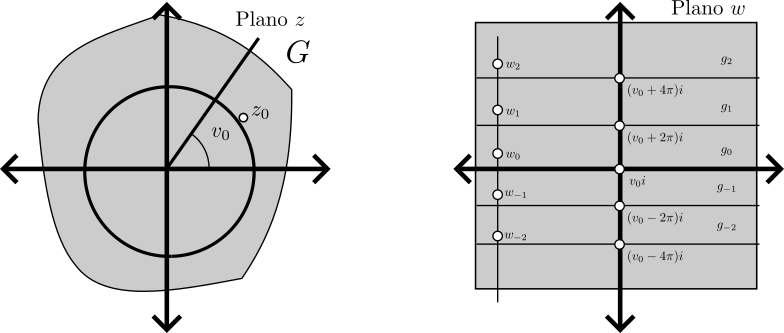
\includegraphics[width=0.7\linewidth]{img/log}
	\caption{Comportamiento del logaritmo complejo}
	\label{fig:log}
\end{figure}

Al igual que la función $w=z^\frac{1}{2}$ revierte el efecto de la función $w_1=z^2$, la función $f(z)=\ln z$ revierte el efecto de la función $g(z)=e^z$
\begin{mmaCell}{Input}
	 f[z_] = Log[z]\\polarConformal[f[r Exp[I t]], \{r, 1, E\}, \{t, 0, 2 Pi\},\\Mesh -> \{30, 30\},LabelStyle -> Directive[Larger, Bold],\\PlotStyle -> White,MeshStyle -> Blue, Axes -> True,\\PlotRange -> \{\{-4, 4\}, \{-4, 4\}\}]
\end{mmaCell}
\begin{mmaCell}[moregraphics={moreig={scale=0.7}}]{Output}
	\mmaFrac{ \mmaGraphics{23.png}}{}
\end{mmaCell}
Como podemos ver en la imagen anterior, el logaritmo regresa el anillo $$\{z\in \C\mid 1<|z|<e\},$$ a la banda vertical $$\{z\in \C|\mbox{Re}(z)\in[0,1],\; \mbox{Im}(z)\in [-\pi,\pi]\}.$$

\section{Transformaciones de Möbius} \label{Möbius}

Comenzamos definiendo lo que es una transformación de Möbius
\begin{defi}
	Un mapeo de la forma 
	\begin{equation}\label{mobius}
		S(z)=\dfrac{az+b}{cz+d},
	\end{equation}
	 es llamada una transformación fraccional lineal. Si  además $a, b, c,$ y $d$ satisfacen que $ad-bc\neq 0$ entonces $S(z)$ es llamada una  transformación de Möbius.
\end{defi}

\begin{prop}\label{prop3}
	El mapeo $S(z)$, definido por la ecuación (\ref{mobius}), es biyectivo y conforme, de
	$$\Omega_{1}=\left\{z\in\C \left|\right. cz+d\neq 0\right\},$$
	sobre 
	$$\Omega_{2}=\left\{w\in\C \left|\right. w\neq \dfrac{a}{c}\right\}.$$
	De hecho, la inversa de $S(z)$ es también una transformación de Möbius dada por
	\begin{equation}\label{invMobius}
		S(w)=\dfrac{dw-b}{a-cw}.
	\end{equation}
Un bosquejo de demostración sería como sigue. Claramente$S(z)$ es analítica en $\Omega_{1}$ y $T(w) = (dw - b)/(a-cw)$ es
analítica en $\Omega_{2}$. El mapeo $S(z)$ será biyectivo si podemos mostrar que $T \circ S$ y $S \circ T$ son la función identidad, ya que esto significa que $S(z)$ tiene a $T(w)$ como su inversa. En efecto, esto se ve en estos cálculos:
\[
\begin{array}{ccl}
	S(T(w))&=&\dfrac{a\left(\dfrac{dw-b}{a-cw} \right) +b}{c\left(\dfrac{dw-b}{a-cw}\right)+d}\\
	&=&\dfrac{-adw+ab+bcw-ab}{-cdw+bc+dcw-da}\\
	&=&\dfrac{(bc-ad)w}{bc-ad}\\
	&=&w.
\end{array}
\]
Note que las cancelaciones realizadas son válidas pues $a-cw\neq  0$ y $bc-ad\neq 0$. Análogamente $T(S(z)) =z$.\\ 
Note que 
$$\dfrac{d}{dz}T(S(z))\dfrac{d}{dz}z=1,$$
y así $$T'(S(z))\cdot S'(z)=1.$$
Por lo tanto, $S'(z)\neq 0$.
\end{prop}
Sean $T(z)=\mobius{a}{+b}{c}{+d}$ y $S(z)=\mobius{e}{+f}{k}{+l}$ dos transformaciones de M\"obius, en Mathematica podemos definirlas como sigue

\begin{mmaCell}{Input}
	 T[z_] = (a z + b)/(c z + d);\\S[z_] = (ez + f)/(kz + l);
\end{mmaCell}
usando la instrucción \textbf{Simplify} podemos obtener la composición de las dos transformaciones de M\"obius anteriores  
\begin{mmaCell}{Input}
	 Simplify[T[S[z]]]
\end{mmaCell}
\begin{mmaCell}[moredefined={f, d}]{Input}
	 \mmaFrac{a f+b l+a e z+b k z}{c f+dl+c e z+d k z}
\end{mmaCell}
Acomodando los términos con el comando \textbf{Collect}
\begin{mmaCell}{Input}
	  Collect[Numerator[\%], z]/Collect[Denominator[\%], z]
\end{mmaCell}

\begin{mmaCell}[moredefined={f, d}]{Input}
    \mmaFrac{a f+b l+(a e+b k) z}{c f+d l+(c e+d k) z}
\end{mmaCell}
Lo anterior demuestra la siguiente 
\begin{prop}
	La composición de dos transformaciones de M\"obius es una transformación
	de M\"obius.
\end{prop}

De hecho, las transformaciones de M\"obius forman un grupo con la operación composición de funciones, recordemos la definición de grupo
\begin{defi}
	Sean $G$  un conjunto no vacío, y $*$ una operación binaria definida en $G$. Se dice que el par $( G , * )$ es un grupo si se cumplen las siguientes condiciones
	\begin{itemize}
		\item [1)] La operación $*$ verifica la propiedad asociativa: dados tres elementos cualesquiera de $g , h , k \in G$, se cumple que $$ (g* h)* k=g* (h*k).$$
		\item [2)] $G$ contiene un elemento distinguido llamado elemento neutro o identidad,6 denotado usualmente como $e$, con la siguiente propiedad: para cualquier $g\in G$
		$$e * g = g * e = g.$$ 
		\item [3)] Todo elemento $ g\in G$ tiene un elemento simétrico o inverso en el mismo  $G$, que se denota por $g^{-1}$, con la propiedad de que $$ g* g^{-1}=g^{-1}* g=e.$$
	\end{itemize}
\end{defi}

\begin{prop}
	El conjunto de transformaciones de M\"obius con la composición de funciones forman un grupo.\\
	Se dará un bosquejo de la demostración apoyándonos del cálculo simbólico de Mathematica. \\
	Sean $T(z)=\mobius{a}{+b}{c}{+d}$, $S(z)=\mobius{e}{+f}{k}{+l}$ y $R(z)=\mobius{m}{+n}{q}{+r}$  transformaciones de M\"obius
	
	\begin{mmaCell}{Input}
		T[z_] = (az + b)/(cz + d);\\S[z_] = (ez + f)/(kz + l);\\R[z_] = (mz + n)/(qz + r);
	\end{mmaCell}
	Realizando la composición $T(S(z))$ en Mathematica 
	\begin{mmaCell}{Input}
		Simplify[T[S[z]]]
	\end{mmaCell}
	\begin{mmaCell}[moredefined={f, d}]{Output}
		\mmaFrac{a f+b l+a e z+b k z}{c f+dl+c e z+d k z}
	\end{mmaCell}


definimos la composición $T(S(z))$ como \textbf{TS[z]}
\begin{mmaCell}[moredefined={f, d}]{Output}
	   TS[z_]=\mmaFrac{af+bl+aez+bkz}{cf+dl+cez+dkz}
\end{mmaCell}
\begin{mmaCell}{Input}
	  Simplify[TS[R[z]]];\\Collect[Numerator[\%], z]/Collect[Denominator[\%], z]
\end{mmaCell}

\begin{mmaCell}[moredefined={f}]{Output}
	   \mmaFrac{aen+bkn+afr+blr+(aem+bkm+afq+blq)z}{dkn+cen+dlr+cfr+(dkm+ce m+dlq+cfq)z}
\end{mmaCell}



por otro lado definimos la composición $S(R(z))$ como \textbf{TS[z]}
\begin{mmaCell}[moredefined={f, d}]{Output}
	  SR[z_]=\mmaFrac{e n+f r+e m z+f q z}{k n+l r+k m z+l q z}
\end{mmaCell}
\begin{mmaCell}{Input}
	 Simplify[T[SR[z]]];\\Collect[Numerator[\%], z]/Collect[Denominator[\%], z]
\end{mmaCell}
\begin{mmaCell}[moredefined={f}]{Output}
    \mmaFrac{aen+bkn+afr+blr+(aem+bkm+afq+blq)z}{dkn+cen+dlr+cfr+(dkm+ce m+dlq+cfq)z}
\end{mmaCell}
lo cual muestra que la operación composición es asociativa.\\
En Mathematica definimos el elemento neutro como
\begin{mmaCell}{Input}
	 Id[z_] = z;
\end{mmaCell}
Entonces 
\begin{mmaCell}{Input}
	 Simplify[Id[T[z]]]
\end{mmaCell}
\begin{mmaCell}{Output}
	 \mmaFrac{b+az}{d+cz}
\end{mmaCell}
análogamente 
\begin{mmaCell}{Input}
	 Simplify[T[Id[z]]]
\end{mmaCell}
\begin{mmaCell}{Output}
	 \mmaFrac{b+az}{d+cz}
\end{mmaCell}
Luego el elemento $Id(z)=z$ es el elemento neutro.\\
Consideremos la transformación $T_1(w)=\dfrac{-b+dw}{z-cw}$ 
\begin{mmaCell}{Input}
	  T1[w_]:=\mmaFrac{-b+dw}{z-cw}
\end{mmaCell}
Realizando la composición 

\begin{mmaCell}{Input}
	  Simplify[T[T1[w]]]
\end{mmaCell}
\begin{mmaCell}{Output}
	 w
\end{mmaCell}
de manera análoga 

\begin{mmaCell}{Input}
	 Simplify[T1[T[z]]]
\end{mmaCell}
\begin{mmaCell}{Output}
	 z
\end{mmaCell}
por tanto el conjunto de transformaciones de M\"obius con la composición de funciones forman un grupo.\endproof
\end{prop}
Sin embargo el grupo de las transformaciones de M\"obius  no es abeliano, por ejemplo tomemos las transformaciones
\[
	\begin{array}{ccl}
		T_1(z)=\dfrac{z}{z+1},&&T_2(z)=\dfrac{z+1}{z-1},
	\end{array}
\]
entonces 
\[
\begin{array}{ccl}
	T_1T_2(z)=\dfrac{z+1}{z},&&T_2T_1(z)=-2z-1,
\end{array}
\]

%%Ejemplo Möbius

\begin{Ejem}\label{ejemplo1}
	Sean $\Omega_{1}=\{x+iy\mid y>0;x,y\in \R\}$ y $\Omega_{2}=D(0,1)$, mostraremos que son conformemente equivalentes. Consideremos 
	$$f(z)=\dfrac{i-z}{i+z},$$
	para $z=x+iy\in\Omega_{1}$, entonces 
	$$f(z)=\dfrac{-x-i(y-1)}{x+i(y+1)},$$
	luego
	$$|f(z)|^2=f(z)\overline{f(z)}=\dfrac{x^2+(y-1)^2}{x^2+(y+1)^2},$$
	como $y>0$ se tiene que $f(z)\in\Omega_{2}$. Además, note que $f$ es analítica en $\Omega_{1}$ ya que $-i\notin\Omega_{1}$, también $f$ es inyectiva. Basta mostrar que $f$ es sobreyectiva.\\
	Sea $w\in\Omega_{2}$, escribamos $w=u+iv$ con $u^2+v^2<1$. Necesitamos encontrar $z\in\Omega_{1}$ tal que $f(z)=w$, es decir, $\dfrac{i-z}{i+z}=w$, resolviendo esta igualdad para $z$ obtenemos $z=i\left(\dfrac{1-w}{1+w}\right)$ y como $w=u+iv$ se tiene que 
	$$z=i\dfrac{(1-u-iv)(1+u-iv)}{(1+u+iv)(1+u+-iv)},$$
	por tanto $$\mbox{Im}(z)=\dfrac{1-u^2-v^2}{(1+u)^2+v^2}>0,$$
	y en consecuencia $z\in\Omega_{2}$.
\end{Ejem}
Las regiones $\Omega_{1}$ y $\Omega_{2}$ se grafican a continuación.
\begin{mmaCell}{Input}
	 omega1 = ComplexRegionPlot[Im[z] >= 0,\\ \{z, -5 - 5 I, 5 + 5 I\}, DisplayFunction -> Identity];
\end{mmaCell}

\begin{mmaCell}{Input}
	 omega2 =ComplexRegionPlot[ Im[I (1 - w)/(w + 1)] >= 0, \\ \{w, -1 - 1 I, 1 + 1 I \},DisplayFunction -> Identity ];
\end{mmaCell}

\begin{mmaCell}{Input}
	 Show[GraphicsGrid[\{\{Graphics[omega1], Graphics[omega2]\}\}, \\\{\}],DisplayFunction -> \$DisplayFunction]
\end{mmaCell}

\begin{mmaCell}[moregraphics={moreig={scale=0.6}}]{Output}
	\mmaFrac{ \mmaGraphics{9.png}}{}
\end{mmaCell}

Si queremos ver la imagen del semiplano superior bajo la función $f(z)=\dfrac{z-1}{z+1}$ que se discutió en el Ejemplo \ref{ejemplo1}, podemos hacerlo con \textbf{cartesianConformal}. Notemos que con esto solo obtenemos, en la imagen de la derecha, solo esa parte del círculo unitario asignada por el tamaño de la malla que en este caso usamos como parámetro \textbf{Mesh}$\rightarrow300$.
\begin{mmaCell}{Input}
	 cartesianConformal[w[x + I*y], \{x, -5, 5\}, \{y, 0, 5\},\\Mesh -> 300,LabelStyle ->Directive[Larger, Bold],\\PlotStyle -> White, MeshStyle -> Blue, Axes -> True,\\PlotPoints ->40, PlotRange -> All]
\end{mmaCell}
\begin{mmaCell}[moregraphics={moreig={scale=0.7}}]{Output}
	\mmaFrac{ \mmaGraphics{10.png}}{}
\end{mmaCell}
Recíprocamente, con la función inversa de $f$, $f^{-1}(z)=i\dfrac{z+1}{z-1}$ podemos ver como se transforma el círculo unitario en el semiplano superior. Para ello usaremos la función \textbf{polarConformal}. La instrucción \textbf{Mesh -> \{300, 300\}} nos indica que el círculo unitario se construirá a partir de 300 círculos concéntricos de radio menor que uno y 300 radios dentro del círculo.
\begin{mmaCell}{Input}
	  polarConformal[f[r Exp[I t]], \{r, 0, 1\}, \{t, 0, 2 Pi\},\\Mesh -> \{300, 300\},LabelStyle -> Directive[Larger, Bold],\\PlotStyle -> White, MeshStyle -> Blue, Axes -> True]
\end{mmaCell}
\begin{mmaCell}[moregraphics={moreig={scale=0.7}}]{Output}
	\mmaFrac{ \mmaGraphics{11.png}}{}
\end{mmaCell}



\begin{defi}
	Sean $\alpha,\beta\in \C$ y $a,\theta\in\R$. Una función $w:\C\rightarrow\C$ se dice que es una 
	\begin{itemize}
		\item [1)] \textbf{Transformación lineal} si $w=\alpha z+\beta$.
		\item [2)] \textbf{Traslación} si $w=z+\beta$.
		\item [3)] \textbf{Estiramiento} si $w=az$.
		\item [4)] \textbf{Inversión} si $w=\dfrac{1}{z}$ si $z\neq0$.
		\item [5)] \textbf{Rotación} si $w=e^{i\theta}z$.
	\end{itemize}
\end{defi}
Estas funciones reciben el nombre de familia fundamental de transformaciones o transformaciones fundamentales.
\begin{Ejem}

Veamos el comportamiento gráfico de las  transformaciones fundamentales usando Mathematica, para ello consideraremos las siguientes transformaciones fundamentales:
\begin{itemize}
	\item [1)] si $w_1=(2-3i) z+ 5+i$,
	\item [2)] si $w_2=z+5+i$,
	\item [3)] si $w_3=4z$,
	\item [4)] si $w_4=\dfrac{1}{z}$ si $z\neq0$,
	\item [5)] si $w_5=e^{\frac{2}{3}\pi i}z$,
\end{itemize}
Usaremos la función \textbf{cartesianConformal} que ya se había construido previamente.
\begin{itemize}
	\item [1)] \begin{mmaCell}{Input}
		 W1[z_] = (2 - 3 I)*z + 5 + I\\cartesianConformal[W1[x + I*y], \{x, -5, 5\}, \{y, 0, 5\},\\Mesh -> 300, LabelStyle -> Directive[Larger, Bold],\\PlotStyle -> White,MeshStyle -> Blue, Axes -> True,\\PlotPoints -> 40,PlotRange -> All]
	\end{mmaCell}
	\begin{mmaCell}[moregraphics={moreig={scale=0.7}}]{Output}
		\mmaFrac{ \mmaGraphics{12.png}}{}
	\end{mmaCell}

	\item [2)] \begin{mmaCell}{Input}
		W2[z_] = z + 5 + I\\cartesianConformal[W2[x + I*y], \{x, -5, 5\}, \{y, 0, 5\},\\Mesh -> 300, LabelStyle -> Directive[Larger, Bold],\\PlotStyle -> White,MeshStyle -> Blue, Axes -> True,\\PlotPoints -> 40,PlotRange -> \{\{-10, 10\}, \{-10, 10\}\}]
	\end{mmaCell}
	\begin{mmaCell}[moregraphics={moreig={scale=0.7}}]{Output}
		\mmaFrac{ \mmaGraphics{13.png}}{}
	\end{mmaCell}

	\item [3)] \begin{mmaCell}{Input}
		W3[z_] = 4*z \\cartesianConformal[W3[x + I*y], \{x, -5, 5\}, \{y, 0, 5\},\\Mesh -> 300, LabelStyle -> Directive[Larger, Bold],\\PlotStyle -> White,MeshStyle -> Blue, Axes -> True,\\PlotPoints -> 40,PlotRange -> \{\{-30, 30\}, \{0, 30\}\}]
	\end{mmaCell}
	\begin{mmaCell}[moregraphics={moreig={scale=0.7}}]{Output}
		\mmaFrac{ \mmaGraphics{14.png}}{}
	\end{mmaCell}

	\item [4)] \begin{mmaCell}{Input}
		W4[z_] = 1/z \\cartesianConformal[W4[x + I*y], \{x, -5, 5\}, \{y, 0, 5\},\\Mesh -> 300, LabelStyle -> Directive[Larger, Bold],\\PlotStyle -> White,MeshStyle -> Blue, Axes -> True,\\PlotPoints -> 40,PlotRange ->\{\{-6, 6\}, \{-6, 6\}\}]
	\end{mmaCell}
	\begin{mmaCell}[moregraphics={moreig={scale=0.7}}]{Output}
		\mmaFrac{ \mmaGraphics{15.png}}{}
	\end{mmaCell}

	\item [5)] \begin{mmaCell}{Input}
		W5[z_] = Exp[2/3 * Pi *I]*z \\cartesianConformal[W5[x + I*y], \{x, -5, 5\}, \{y, 0, 5\},\\Mesh -> 300, LabelStyle -> Directive[Larger, Bold],\\PlotStyle -> White,MeshStyle -> Blue, Axes -> True,\\PlotPoints -> 40,PlotRange ->\{\{-7, 7\}, \{-7, 7\}\}]
	\end{mmaCell}
	\begin{mmaCell}[moregraphics={moreig={scale=0.7}}]{Output}
		\mmaFrac{ \mmaGraphics{16.png}}{}
	\end{mmaCell}
\end{itemize}
	
\end{Ejem}
Note que gráficamente  una transformación de M\"obius se puede obtener a partir de aplicar distintas transformaciones fundamentales sucesivamente, formalmente 
\begin{prop}\label{prop4}
	Una transformación de M\"obius es la composición de transformaciones fundamentales.\\
	La prueba de esta proposición no es difícil, a continuación se da un esbozo de la demostración.\\ Sea $S(z)=\mobius{a}{+b}{c}{+d}$. Si $c=0$, entonces $S(z)=\dfrac{a}{d}z+\dfrac{b}{d}$, la cual es una transformación lineal.\\
	Si $c\neq 0$, entonces 
	\[
		\begin{array}{ccl}
			S(z)&=&\mobius{a}{+b}{c}{+d}\\
			&=&\dfrac{c^2(az+b)}{c^2(az+b)}\\
			&=&\dfrac{ac^2z + bc^2 + adc - adc}{c^2(az+b)}\\
			&=&\dfrac{ac(cz+d)+c(bc-ad)}{c^2(az+b)}\\
			&=&\dfrac{a}{c}+\dfrac{bc-ad}{c(cz+d)}\\
			&=&\alpha +\dfrac{\beta}{z+\gamma},
		\end{array}
	\]
	donde $\alpha=\dfrac{a}{c}$, $\beta=\dfrac{bc-ad}{c^2}$ y $\gamma=\dfrac{d}{c}$.\endproof
\end{prop}
El siguiente teorema es quizás uno de los mas importantes en el análisis complejo pues establece, en palabras simples, que dado todo subconjunto propio abierto sin agujeros del plano complejo se puede "meter" $\;$dentro de un disco abierto unitario. Este teorema fue enunciado  por Bernhard Riemann en 1851 en su tesis doctoral y aunque Riemann dio una prueba del teorema, esta no resulto ser correcta, no fue sino hasta 1900 cuando William Fogg Osgood dio la primera demostración rigurosa del teorema.

\begin{teor}[del mapeo de Riemann]\label{TMR}
	Sea $\Omega$ una región simplemente conexa tal que $\Omega\neq \C$. Entonces existe un mapeo conforme biyectivo $f: \Omega\rightarrow D$, donde $D =\{ z : |z| < 1 \}$.
	\proof
	La demostración se puede consultar en \cite{tarlok} página 85, Teorema 3.10.\endproof
\end{teor}
Bajo ciertas condiciones la función que se enuncia en el Teorema \ref{TMR} es única
\begin{prop}\label{propTMR}
 Asuma que $\Omega$ satisface las suposiciones del Teorema \ref{TMR} y sea $z_0\in \Omega$. Entonces existe una única función $f:\Omega\rightarrow D$ tal que  $f\in \mathcal{H}(\Omega)$, $f$ es inyectiva y $f(z_0)$ con $f'(z_0)>0$.
 \proof Vea la demostración en  \cite{tarlok}, Teorema 3.18 página 94.\endproof
\end{prop}

\begin{coro}\label{coroRiemman}
	 Asuma que $\Omega$ satisface las suposiciones del Teorema \ref{TMR} y sean $z_0\in \Omega$, $w_0\in D$ y un ángulo $\theta_0$ y al asumir la Proposición \ref{propTMR}, demuestre que existe un mapeo conforme $f:\Omega\rightarrow D$ tal que $f(z_0)=w_0$ y $\mbox{arg}f'(z_0)=\theta_0$, y además $f$ es único.
\end{coro}

\begin{teor}[del módulo máximo]\label{modmx}
	Suponga que $f (z)$ es analítica en el interior y sobre una curva simple cerrada $C$. Así, el valor máximo de $| f (z)|$ se encuentra sobre $C$, a menos que $f (z)$ sea una constante.
	\proof La demostración se puede consultar en \cite{marsden}, Teorema 6.3.5.\endproof
\end{teor}
\begin{prop}
	Cualquier mapeo conforme de $D =\{ z : |z| < 1 \}$ sobre sí mismo es un mapeo de la forma de la forma
	$$T(z)=e^{i\theta}\dfrac{z-z_{0}}{1-\bar{z_{0}}z},$$
	para alguna $z_{0}\in D$ fija y $\theta \in [0, 2\pi[$; más aún, cualquier $T$ de esta forma es un mapeo conforme de $D$ sobre $D$, y además $T$ es único. 
	\proof
	La demostración la podemos consultar en \cite{marsden}, ver la Proposición  5.2.2. \endproof

\end{prop}
Notemos que la transformación lineal entera $w = az+b$ $(a\neq 0)$ claramente preserva círculos, ya que el mapeo $w$ es solo una traslación  (si $a = 1)$, o una traslación combinada con un estiramiento (si $a\neq 1$).
\begin{lema}\label{lema1}
	La transformación
	$$w=\dfrac{1}{z},$$
	preserva círculos.\\
Una forma de probar el lema anterior es usar la proyección estereográfica y utilizar el hecho de que esta manda rectas o círculos del plano en círculos de la esfera y
que la inversa manda círculos de la esfera en rectas o círculos del plano. Un bosquejo de la demostración sería como sigue.\\
Sea $\pi(z)=(x_1,x_2,x_3)$ un punto de la esfera $S^2$ , tomemos $z=x+iy$ en el plano $Z$ y $w=\dfrac{1}{z}=\dfrac{\overline{z}}{z\overline{z}}=\dfrac{x-iy}{x^2+y^2}$ en el plano $W$. Tenemos que 
$$|w|^2=\dfrac{1}{x^2+y^2}\implies |w|^2+1=\dfrac{x^2+y^2+1}{x^2+y^2}.$$
Utilizando las coordenadas en la esfera el punto $w$ se tiene 
$$y_1=\dfrac{w+\overline{w}}{1+|w|^2}=\dfrac{2x}{|z|^2+1}=x_1,$$
$$y_1=\dfrac{w-\overline{w}}{i(|w|^2+1)}=-\dfrac{2iy}{i(|z|^1+1)}=-x_2,$$
$$y_3=\dfrac{|w|^2-1}{|w|^2+1}=\dfrac{1-|z|^2}{1+|z|^2}=-x_3,$$
es decir, si miramos a $w=\dfrac{1}{z}$ como la acción bajo la proyección estereográfica, $w$ vista en la esfera deja fija la coordenada $x_1$, luego es una rotación de $x_2$ a $-x_2$ y otra rotación  de $x_3$ a $-x_3$, ambas acciones preservan círculos en la esfera. De aquí se sigue el resultado
\end{lema}

\begin{prop}
	Toda transformación de M\"obius 
	\begin{equation}\label{trmob}
		T(z)=w=\mobius{a}{+b}{c}{+d},
	\end{equation}
	preserva círculos.\\
	La prueba de esta proposición es consecuencia del Lema \ref{lema1}, a continuación, se da un bosquejo.\\
	Si $c=0$ es resultado es claro. Consideremos el caso cuando $c\neq0$, entonces $w$ se puede escribir de la forma 
	$$w=\dfrac{a}{c}+\dfrac{bc-ad}{c(cz+d)},$$
	si $z_1=L_1(z)=cz+d$ y $z_2=L_2=\dfrac{1}{z_1}$ entonces 
	$$L_3(z_2)=\dfrac{a}{c}+\dfrac{bc-ad}{c}z_2,$$
	luego $w$ se puede escribir como el producto $$w=L_3L_2L_1,$$ de tres transformaciones que preservan círculos. Luego $T$ preserva círculos.
\end{prop}
\begin{coro}
	Sea $\delta=-\dfrac{d}{c}$ el polo de la transformación de M\"obius $$T(z)=w=\mobius{a}{+b}{c}{+d}.$$ Entonces la transformación $T$ transforma toda recta o círculo que pasa a través de $\delta$ en una recta,  y cualquier otra línea recta o círculo en	un circulo.
\end{coro}
Consideremos la transformación de M\"obius $$T(z)=\mobius{5}{+(5+3i)}{(2.4+3.2i)}{+{4.3+7.2i}}$$
y el disco $D=\{z\in \C: |z|< 1\}$
Podemos usar la función \textbf{polarConformal} para comprobar visualmente la proposición anterior
\begin{mmaCell}{Input}
	 TMobius[z_, a_, b_, c_, d_] = (a*z + b)/(c*z + d);\\polarConformal[ TMobius[r Exp[I t], 5, 5 + 3 I,\\2.4 + 3.2 I, 4.3 + 7.2 I],\\\{r, 0, 1\}, \{t, 0, 2 Pi\},Mesh->\{0, 0\},\\PlotRange ->Automatic,LabelStyle-> Directive[Larger,Bold],\\PlotStyle -> White,MeshStyle -> Blue, Axes -> True]
\end{mmaCell}
\begin{mmaCell}[moregraphics={moreig={scale=0.7}}]{Output}
	\mmaFrac{ \mmaGraphics{27.png}}{}
\end{mmaCell}

Consideremos los puntos $z_{1}, z_{2}, z_{3}$ en el plano $z$ y respectivamente los puntos $w_{1}, w_{2}, w_{3}$ en el plano $W$. Si $w_k$ corresponde a $z_k$, $k=1,2,3$, se tiene 
$$w-w_k=\mobius{a}{+b}{c}{+d}-\dfrac{az_k+b}{cz_k+d}=\dfrac{(ad-bc)(z-z_k)}{(cz+d)(cz_k+d)},$$
así que 
\[
	\begin{array}{cc}
		w-w_1=\dfrac{(ad-bc)(z-z_1)}{(cz+d)(cz_1+d)},&w-w_3=\dfrac{(ad-bc)(z-z_3)}{(cz+d)(cz_3+d)},
	\end{array}
\]
Sustituyendo $w$ por $w_2$ y $z$ por $z_2$,
\[
\begin{array}{cc}
	w_2-w_1=\dfrac{(ad-bc)(z_2-z_1)}{(cz_2+d)(cz_1+d)},&w_2-w_3=\dfrac{(ad-bc)(z_2-z_3)}{(cz_2+d)(cz_3+d)}.
\end{array}
\]
Si suponemos que $ad-bc\neq 0$, entonces 
\begin{equation}\label{razoncruzada}
	\dfrac{(w-w_1)(w_2-w_3)}{(w-w_3)(w_2-w_1)}=\dfrac{(z-z_1)(z_2-z_3)}{(z-z_3)(z_2-z_1)}.
\end{equation}
Si se despeja $w$ en términos de $z$ y se obtiene una transformación de M\"obius $S$ que manda $z_i \rightarrow w_i$, $i = l , 2, 3$. Se ha demostrado la siguiente
\begin{prop}[Razón cruzada]
	Dados dos conjuntos de puntos distintos $z_{1}, z_{2}, z_{3}$ y $w_{1}, w_{2}, w_{3}$, existe una única transformación de M\"obius $S$ que manda $z_i \rightarrow w_i$, $i = l , 2, 3$, De hecho, si $S(z) = w$, entonces $$\dfrac{(w-w_1)(w_2-w_3)}{(w-w_3)(w_2-w_1)}=\dfrac{(z-z_1)(z_2-z_3)}{(z-z_3)(z_2-z_1)}.$$
\end{prop}
\subsection{Transformaciones de M\"obius en el plano extendido}

Consideremos la transformación 
\begin{equation}\label{mob}
	w=\mobius{a}{+b}{c}{+d},
\end{equation} 
Cuando un punto $w$ es la imagen de algún punto $z$ bajo la transformación (\ref{mob}), el punto $z$ se recupera por medio de la transformación (\ref{invMobius}).\\
Si $c=0$, de modo que $a\neq 0$, $d\neq 0$, cada punto en el plano $W$ es la imagen de uno y solo un punto en el plano $Z$. Lo mismo es cierto si  $c\neq 0$, excepto cuando $w=\dfrac{a}{c}$ ya que el denominador de la ecuación (\ref{invMobius}) se anula si $w$ tiene ese valor, sin embargo, podemos ampliar el dominio que se dio en la Proposición \ref{prop3} para las trasformaciones de M\"obius para definir una trasformación de M\"obius  en el plano extendido
$$\bar{\C}=\C\cup \{\infty\},$$
tal que el punto $w=\dfrac{a}{c}$ es la imagen de $z=\infty$ cuando $c\neq 0$, la definición de esta transformación sería la siguiente 

\[
	S(z)=\left\{ \begin{array}{ccl}
		\mobius{a}{+b}{c}{+d},& &\mbox{ si } z\in \C\setminus\left\{-\dfrac{d}{c}\right\}\\\\
		\dfrac{a}{c},& &\mbox{ si } z=\infty\\\\
		\infty,& &\mbox{ si } z=-\dfrac{d}{c},
	\end{array} \right.
\]
y si $c=0$, 
\[
S(z)=\left\{ \begin{array}{ccl}
	\dfrac{a}{d}z+\dfrac{b}{d},& &\mbox{ si } z\in \C\\
	\infty,& &\mbox{ si } z=\infty,
\end{array} \right.
\]
No es difícil ver que los siguientes límites se cumplen
\[
\begin{array}{ccl}
	\ds\lim_{z\rightarrow\infty}S(z)= \infty,&&\mbox{ si } c=0,\\
	\ds\lim_{z\rightarrow\infty}S(z)= \dfrac{a}{c},&&\mbox{ si } c\neq0,\\
	\ds\lim_{z\rightarrow -\dfrac{d}{c}}S(z)= \infty,&&\mbox{ si } c\neq 0,
\end{array}
\] 
lo cual muestra que las transformaciones de M\"obius definidas de esta forma son continuas en el plano extendido. Asimismo, en el plano extendido las transformaciones definidas ahí también resultan ser biyecciones. Por lo tanto, podemos habar de la transformación de M\"obius inversa
definida de la siguiente forma

\[
S^{-1}(w)=\left\{ \begin{array}{ccl}
	\infty,& &\mbox{ si } w=\infty \mbox{ y } c=0\\
	\infty,& &\mbox{ si } w=\dfrac{a}{c} \mbox{ y } c\neq0\\
	-\dfrac{d}{c},& &\mbox{ si } w=\infty \mbox{ y } c\neq0.
\end{array} \right.
\]
\begin{Ejem}
	Considere los puntos $z_1=1$, $z_2=0$, $z_3=-1$ y $w_1=i$, $w_2=\infty$, $w_3=1$, en este caso la fórmula de la razón cruzada quedaría de la siguiente manera
	$$\dfrac{w-w_1}{w-w_3}=\dfrac{(z-z_1)(z_2-z_3)}{(z-z_3)(z_2-z_1)},$$
	sustituyendo valores quedaría como
	$$\dfrac{w-i}{w-1}=\dfrac{(z-1)(0+1)}{(z+1)(0-1)},$$
	despejando para $w$ se obtiene 
	$$w=\dfrac{(i+1)z+(i-1)}{2z},$$
\end{Ejem}
A continuación implementamos el método de la razón cruzada en Mathematica
\begin{mmaCell}{Input}
	 Mobius[z_, a_, b_, c_, d_] := (a z + b)/(c z + d)\\
\end{mmaCell}
\begin{mmaCell}{Input}
	 Clear[RazonCruzada, za, zb, zc, wa, wb, wc]\\RazonCruzada[z_, \{za_, zb_, zc_\}, \{wa_, wb_, wc_\}] :=\\Module[\{soln\},soln = Solve[\{wa == Mobius[za, a, b, c, 1],\\wb == Mobius[zb, a, b, c, 1], wc == Mobius[zc,a,b,c,1]\},\\\{a,b,c\}];\\Mobius[z, a, b, c, 1] /. soln[[1]]]
\end{mmaCell}
Consideremos nuevamente los puntos $z_1=1$, $z_2=0$, $z_3=-1$ y $w_1=i$, $w_2=\infty$, $w_3=1$ pero esta vez $w_2= t$ y aplicaremos el límite cuando $t\rightarrow\infty$
\begin{mmaCell}{Input}
	   RazonCruzada[z, {1, 0, -1}, {I, t, 1}]
\end{mmaCell}
\begin{mmaCell}[moredefined={t}]{Output}
	  \mmaFrac{t-i ((-1-i)+t) z}{1+(i-(1+i) t) z}
\end{mmaCell}
Tomando el límite 
\begin{mmaCell}[moredefined={t}]{Input}
	 Limit[\mmaFrac{t-i ((-1-i)+t) z}{1+(i-(1+i) t) z},t -> Infinity]\\Collect[Numerator[%], z]/Collect[Denominator[%], z]
\end{mmaCell}
\begin{mmaCell}{Input}
	 \mmaFrac{(-1+i)+(1+i) z}{2 z}
\end{mmaCell}

\section{Mapeo de Joukowski} \label{Joukowski}


\begin{Ejem}
	Encuentre las líneas de corriente para el flujo alrededor de un obstáculo cilíndrico centrado en el origen y de radio $R$.
	\solu
	Por un momento supongamos que el flujo es simétrico con respecto al eje $x$. Basta estudiar el flujo cuando $y\geq 0$. Para mapear la región de flujo en el semiplano superior necesitamos una función analítica $f(z)$ que sea real al menos para $|x|>R$ y en el círculo $|z|=R$. La primera condición se cumple para las funciones racionales con coeficientes reales, para la segunda condición notemos que el círculo puede ser descrito por
	$$z\bar{z}=R^2,$$
	se tiene así que $\bar{z}=\dfrac{R^2}{z}$, por lo tanto la función racional $z+\dfrac{R^2}{z}$ es igual a $z+\bar{z}="\mbox{Re}z$  en el círculo, en consecuencia tenemos el mapeo
	$$w=f(z)=z+\dfrac{R^2}{z}.$$
	Esta función es un mapeo inyectivo de la región de flujo para $y>0$ sobre el semiplano superior. Por lo tanto, la función de flujo apropiada corresponde a $\psi(u, v) = v = \mbox{Im}w$, dando las líneas de corriente
	$$\varphi(x,y)=\mbox{Im}\left(z+\dfrac{R^2}{z}\right)=\mbox{cte}.$$\endsolu
	
\end{Ejem}



Si eliminamos el supuesto que el flujo sea simétrico, entonces solo requerimos que el círculo mismo sea una línea de corriente. Por lo tanto podemos agregar cualquier múltiplo constante  de $\log |z|$ (ya que se tiene que $|z|=R$ es una línea de corriente) a la función de corriente y obtener los patrones de flujo circulante.\\

En 1908 el matemático Nikolái Zhukovski  (a veces escrito Joukowski) estudio este tipo de mapeos pero no aplicados al círculo $|z|=R$, si no a círculos $C$ cuyo centro fuera distinto al origen. El resultado que obtuvo fue un perfil aerodinámico como el de la figura \ref{fig:24}.\\Al comenzar con diferentes círculos C podemos generar una variedad de estos llamados perfiles aerodinámicos de Joukowski, podemos usar la transformación de Joukowski para calcular los flujos alrededor de distintos perfiles aerodinámicos. Por ejemplo, podemos dar forma al perfil aerodinámico para cumplir con ciertas especificaciones de ingeniería eligiendo adecuadamente $C$ e introduciendo modificaciones en el mapeo como, por ejemplo:
$$w=f(z)=z+\dfrac{R^2}{z}+\dfrac{a}{z^2}+\dfrac{b}{z^2}+\cdots$$
\begin{figure}[h!]
	\centering
	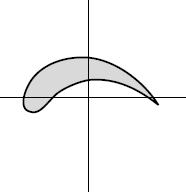
\includegraphics[width=0.2\linewidth]{img/24}
	\caption{Perfil aerodinámico}
	\label{fig:24}
\end{figure}
 

Consideremos ahora el mapeo 
\begin{equation}
	w=J(z)=\dfrac{1}{2}\left(z+\dfrac{1}{z}\right)=\dfrac{z^2+1}{2z},
\end{equation}
no es difícil ver que 
\begin{equation}\label{derj}
	J(z)=J\left(\dfrac{1}{z}\right).
\end{equation}
Además tenemos que $J(0)=J(\infty)=\infty$. \\
Derivando obtenemos $$J'(z)=\dfrac{1}{2}\left(z-\dfrac{1}{z^2}\right).$$
Luego $J'(z)=0$ si y sólo si $z=\pm 1$, por lo que $J$ es conforme en $\C\setminus\{0,\pm 1\}$. Por otro lado, si $J(z_1)=J(z_2)$ entonces $z_{1}^2z_2+z_2=z_{2}^2+z_1$, luego $(z_1-z_2)(z_1z_2-1)=0$ de donde $z_1=z_2$ o $z_1z_2=1$, es decir, que cada punto del plano $W$ tiene en la transformación $w$ dos preimágenes $z_1$ y $z_2$ ligadas por la relación $z_1z_2=1$. Si una de éstas preimágenes pertenece al interior del círculo unitario, la otra pertenece al exterior  y viceversa. A continuación, veremos como el mapeo $J(z)$ transforma dominio $D=\{z\in \C\mid |z|\leq 1 \}$ en un dominio $G$ de del plano $W$ muy parecido a un perfil aerodinámico. Veamos primero la imagen de la frontera de $D$, $$\partial D=\{z\in\C\mid |z|=1\}.$$
Si $z=e^{it}$, con $t\in[0,2\pi]$, entonces $J(e^{it})=\dfrac{1}{2}\left(e^{it}+e^{-it}\right)=\cos t$, es decir, la imagen de $\partial D$ bajo $J$ es el segmento del eje real $[-1,1]$ recorrido dos veces. Por lo que, se puede afirmar que $G$ está formado por todos aquellos puntos del plano $W$  a excepción de aquellos que pertenecen al segmento del eje real $[-1,1]$. En efecto, consideremos las imágenes de las circunferencias $|z|=r$ y los radios $\mbox{Arg}\; z=\alpha+2k\pi$, consideremos solo el interior de $D$, $(D^{\circ})$. Tomando el cambio $z=re^{it}$ con $t\in[0,2\pi]$ y $r\in (0,1)$, entonces
$$J(z)=J(re^{it})=\dfrac{1}{2}\left(r+\dfrac{1}{r}\right)\cos t-i\dfrac{1}{2}\left(\dfrac{1}{r}-r\right)\sen t,$$
o bien 
$$u=\dfrac{1}{2}\left(r+\dfrac{1}{r}\right)\cos t,$$
$$v=\dfrac{1}{2}\left(r-\dfrac{1}{r}\right)\sen t,$$
de donde obtenemos 
\begin{equation}\label{ecelip}
	\dfrac{u^2}{\left[\dfrac{1}{2}\left(r+\dfrac{1}{r}\right)\right]^2} +\dfrac{v^2}{\left[\dfrac{1}{2}\left(\dfrac{1}{r}-r\right)\right]^2}=1.
\end{equation}
Esta es la ecuación de una elipse con los semiejes $a=\dfrac{1}{2}\left(r+\dfrac{1}{r}\right)$ y $b=\dfrac{1}{2}\left(\dfrac{1}{r}-r\right)$; y los focos $\pm 1$. De las ecuaciones para $u$ y $v$; y (\ref{ecelip}) se deduce que, cuando $t$ crece continuamente desde $0$ hasta $2\pi$, el punto correspondiente describe una vez la elipse (\ref{ecelip}) en dirección negativa. En efecto, cuando $t\in[0,\frac{\pi}{2}]$, $u$ es positivo y decrece desde $a$ hasta $0$, mientras que $v$ es negativo y decrece desde $0$ hasta $-b$; cuando $t\in(\frac{\pi}{2},\pi)$, $u$ continúa decreciendo desde $0$ hasta $-a$, mientras que $v$ decrece desde $-b$ hasta $0$; cuando $t\in (\pi ,\frac{3\pi}{2})$, $u$ crece desde $-a$ hasta $0$, mientras que $v$ crece desde $0$ hasta $b$; finalmente, cuando $t\in (\frac{3\pi}{2},2\pi)$, $u$ crece desde $0$ hasta $a$, mientras que $v$ decrece desde $b$ hasta $0$.\\
Variando el radio $r$ de la circunferencia $|z|=1$ desde $0$ hasta $1$, hacemos decrecer a $a$ desde $\infty$ hasta $1$ y $b$, desde $\infty$ a $0$; las elipses correspondientes describirán todo el conjunto de elipses del plano $W$ con los focos $\pm 1$. De aquí se deduce que $J(z)$ transforma biunívocamente  el círculo unitario es el conjunto $G$ que representa el exterior del segmento $[-1,1]$.\\
Para la imagen del radio $z=te^{i\alpha}$, $t\in[0,1]$, primero obtenemos la ecuación 
\begin{equation}\label{echip}
	J(z)=\dfrac{1}{2}\left(\dfrac{1}{t}+t\right)\cos \alpha-i\dfrac{1}{2}\left(\dfrac{1}{t}-t\right)\sen \alpha,
\end{equation}
de donde 
$$u=\dfrac{1}{2}\left(\dfrac{1}{t}+t\right)\cos \alpha,$$
$$v=-\dfrac{1}{2}\left(\dfrac{1}{t}-t\right)\sen \alpha,$$
de aquí vemos que las imágenes de dos radios, simétricos respecto del eje real, también son simétricos respectos del eje real, mientras que las imágenes de dos radios, simétricos respecto del eje imaginario, son simétricos respecto al eje imaginario. Es por ello que basta considerar solamente la imágenes de los radios pertenecientes al cuadrante $0\leq \alpha\leq \dfrac{\pi}{2}$.\\
Para $\alpha=0$ tenemos 
$$u=0,$$
$$v=-\dfrac{1}{2}\left(\dfrac{1}{t}-t\right),$$
con $t\in[0,1]$. Estos es un subintervalo infinito del eje real: $1<u<\infty$. El intervalo simétrico a éste $-\infty<u<-1$ es la imagen del radio que corresponde a $\alpha=\pi$.\\
Para $\alpha=\dfrac{\pi}{2}$, se tiene: 
$$u=0,$$
$$v=-\dfrac{1}{2}\left(\dfrac{1}{t}-t\right),$$
con $t\in[0,1]$. Este es el semieje imaginario $-\infty<v<0$. El otro semieje imaginario $0<v<\infty$ es la imagen del radio que corresponde a $\alpha=-\dfrac{\pi}{2}$.\\
Supongamos ahora que $0<\alpha<\dfrac{\pi}{2}$. Entonces de las ecuaciones para $u,v$ y (\ref{echip}) se obtiene
\begin{equation}\label{elipse}
	\dfrac{u^2}{\cos^{2}\alpha}-\dfrac{v^2}{\sen^{2}\alpha}=1.
\end{equation}
Esta es la ecuación de una hipérbola $H$ con el semieje real $a=\cos \alpha$; con semieje imaginario $b=\sen \alpha$ y con los focos $\pm 1$. Sea $H_k$ la intersección de $H$ con el $i$-ésimo cuadrante para cada $i=1,2,3,4$ respectivamente, excluyendo los puntos $(\pm a,0)$ de $H$ que pertenecen al eje real. Además, sean $R_{\alpha}$, $R_{\pi-\alpha}$, $R_{\pi+\alpha}$ y $R_{-\alpha}$ los conjuntos de puntos que pertenecen al radio $z=te^{i\alpha}$ con inclinaciones $\alpha$, $\pi-\alpha$, $\pi +\alpha$ y $-\alpha$ respectivamente. Tenemos que 
\[
	\begin{array}{cccc}
		H_1=J(R_{-\alpha}),&H_2=J(R_{\pi + \alpha}),&H_3=J(R_{\pi -\alpha}), &H_4=J(R_{\alpha}).
	\end{array}
\]
Note que la imagen de cada uno de los diámetros formados por estos radios será la parte de la $H$ formada por los pares de sus cuartas partes que son simétricas respecto del origen de coordenadas y que están ligadas entre sí en el punto del infinito.\\
Resumiendo, la función $J(z)$ transforma biunívocamente tanto el interior como el exterior del círculo unidad en el exterior del segmento $-1\leq u \leq 1$ (del eje real).  En este caso, las circunferencias $|z|=r$ se transforman en elipses con los focos $\pm1$ y semiejes $\dfrac{1}{2}\left|\dfrac{1}{r}\pm r \right|$, y los pares de diámetros simétricos respecto de los ejes coordenados formados por los radios $z=\pm re^{i\alpha}$ donde $0<\alpha<\dfrac{\pi}{2}$ se transforman en hipérbolas con los focos $\pm 1$ y semiejes $|\cos\alpha|$, $|\sen\alpha|$ a excepción de los vértices de estas hipérbolas. 

\subsection{Mapeo de Joukowski usando Mathematica} \label{Joukowski-mathematica}
La siguiente implementación en Mathematica se tomo de \cite{GeometryJo}.

\begin{mmaCell}{Input}
	 rotationTransform[\mmaPat{\(\pmb{\zeta}\)_},\mmaPat{\(\pmb{\alpha}\)_}]:=\mmaPat{\(\pmb{\zeta}\)} \mmaSup{\mmaDef{e}}{\mmaDef{i} \mmaPat{\(\pmb{\alpha}\)}}
\end{mmaCell}

\begin{mmaCell}[moredefined={translationTransform}]{Input}
	 translationTransform[\mmaPat{\(\pmb{\zeta}\)_},\mmaPat{\(\pmb{\mu}\)_}]:=\mmaPat{\(\pmb{\zeta}\)}+\mmaPat{\(\pmb{\mu}\)}
\end{mmaCell}
\begin{mmaCell}[moredefined={joukowskiTransform}]{Input}
	 joukowskiTransform[\mmaPat{\(\pmb{\zeta}\)_}]:=0.5* (\mmaPat{\(\pmb{\zeta}\)}+\mmaFrac{1}{\mmaPat{\(\pmb{\zeta}\)}})
\end{mmaCell}
\begin{mmaCell}{Input}
	 Function[\mmaPat{\(\pmb{\zeta}\)},0.5*(\mmaPat{\(\pmb{\zeta}\)}+\mmaFrac{1}{\mmaPat{\(\pmb{\zeta}\)}})]
\end{mmaCell}
\begin{mmaCell}[morelocal={a}]{Input}
	 \mmaDef{\(\pmb{\zeta}\)0C}[\mmaPat{\(\pmb{\theta}\)_},\mmaPat{\(\pmb{\mu}\)_}]:=Module[\{a,\mmaLoc{\(\pmb{\beta}\)}\},\{a,\mmaLoc{\(\pmb{\beta}\)}\}=\{Abs[1-\mmaPat{\(\pmb{\mu}\)}],-Arg[1-\mmaPat{\(\pmb{\mu}\)}]\};\\a \mmaSup{\mmaDef{e}}{-\mmaDef{i} (\mmaPat{\(\pmb{\theta}\)}+\mmaLoc{\(\pmb{\beta}\)})}]
\end{mmaCell}
\begin{mmaCell}[moredefined={translationTransform}]{Input}
	 \mmaDef{\(\pmb{\zeta}\)C}[\mmaPat{\(\pmb{\theta}\)_},\mmaPat{\(\pmb{\mu}\)_}]:=translationTransform[\mmaDef{\(\pmb{\zeta}\)0C}[\mmaPat{\(\pmb{\theta}\)},\mmaPat{\(\pmb{\mu}\)}],\mmaPat{\(\pmb{\mu}\)}]
\end{mmaCell}
\begin{mmaCell}[moredefined={zA, joukowskiTransform}]{Input}
	 zA[\mmaPat{\(\pmb{\theta}\)_},\mmaPat{\(\pmb{\mu}\)_}]:=joukowskiTransform[\mmaDef{\(\pmb{\zeta}\)C}[\mmaPat{\(\pmb{\theta}\)},\mmaPat{\(\pmb{\mu}\)}]]
\end{mmaCell}
\begin{mmaCell}[moredefined={zA}]{Input}
	\mmaDef{\(\pmb{\theta}\)LE}[\mmaPat{\(\pmb{\mu}\)_}]:=\mmaUnd{\(\pmb{\theta}\)}/.\(\pmb{\,}\)FindRoot[Im[zA[\mmaFnc{\(\pmb{\theta}\)},\mmaPat{\(\pmb{\mu}\)}]],\{\mmaFnc{\(\pmb{\theta}\)},\mmaDef{\(\pmb{\pi}\)}\}]
\end{mmaCell}

\begin{mmaCell}[moredefined={xLE, zA}]{Input}
	xLE[\mmaPat{\(\pmb{\mu}\)_}]:=Chop[zA[\mmaDef{\(\pmb{\theta}\)LE}[\mmaPat{\(\pmb{\mu}\)}],\mmaPat{\(\pmb{\mu}\)}]]
\end{mmaCell}



\begin{mmaCell}[moregraphics={moreig={scale=0.6}}]{Input}
	\mmaFrac{ \mmaGraphics{program.png}}{}
\end{mmaCell}


Lo  que el script anterior genera es una forma de ver como el círculo se deforma en perfiles aerodinámicos y además proporciona unos controles para variar el tamaño del círculo y apreciar en tiempo real como se produce un nuevo perfil aerodinámico. La forma del perfil aerodinámico está controlada por un triángulo de referencia en el plano $Z$ definido por el origen, el centro del círculo  $z=re^{i\alpha}$ y el punto $z=1$.
\begin{mmaCell}[moregraphics={moreig={scale=0.6}}]{Input}
	\mmaFrac{ \mmaGraphics{perfiles1.png}}{}
\end{mmaCell}




\section{Mapeo de Schwarz-Christoffel}
El Teorema del mapeo de Riemann nos dice que cualquier región simplemente conexa $\Omega$, estrictamente contenida en el plano complejo, podría ser transformada conformemente en el disco unitario abierto $D$ del plano complejo (Teorema \ref{TMR}), sin embargo este teorema de existencia no es constructivo, es decir, no se proporciona un método explicito para encontrar tal mapeo conforme.\\
En esta sección se realiza un breve estudio del mapeo de Schwarz–Christoffel, este mapeo se define por una serie de puntos singulares en el borde del polígono y su correspondencia con puntos en el eje real del semiplano. La función de mapeo se construye a partir de una fracción algebraica que se integra en una función analítica específica. Además, el mapeo de Schwarz-Christoffel es una herramienta valiosa para la visualización y la solución de problemas en muchas áreas de la matemática, incluyendo la teoría de números, la teoría de sistemas dinámicos y la teoría de grupos. También es importante en la aplicación del cálculo numérico y la teoría de la optimización en la solución de problemas en ingeniería y ciencias.\\

Además, el mapeo de Schwarz-Christoffel tiene propiedades únicas que lo hacen diferente de otras transformaciones conformes. Por ejemplo, es posible calcular el área y la longitud de curvas en un polígono a partir de su representación en un semiplano, lo que es útil para resolver problemas en geometría y teoría de curvas.
Consideremos una región simplemente conexa $\Omega$, cuya frontera sea un polígono de $n$ lados en el plano $W$ con vértices $w_1,w_2,\ldots,w_n$, en 1866 Hermann Amandus Schwarz e independientemente en 1867  Elwin Bruno Christoffel, publicaron una forma de mapear  el semiplano superior en  la región $\Omega$.
\begin{figure}[h!]
	\centering
	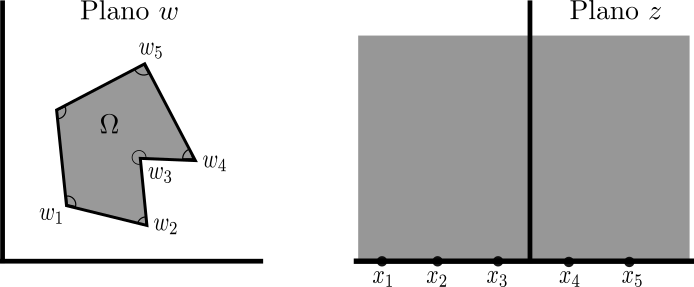
\includegraphics[width=0.7\linewidth]{img/sc}
	\caption{Transformación de Schwarz-Christoffel}
	\label{fig:sc}
\end{figure}
Suponga que cada $w_j$ se mapea en $x_j$, donde $x_j$ es un punto en el eje real.
La transformación que mapea el semiplano superior en   $\Omega$ está definida  como 

\begin{equation}\label{dSC}
	\dfrac{dw}{dz}=C_1\prod_{j=1}^{n}(z-x_n)^{\frac{\phi_j}{\pi}-1}.
\end{equation}
En forma integral
\begin{equation}\label{eSC}
	w=C_1\int \prod_{j=1}^{n}(z-x_n)^{\frac{\phi_j}{\pi}-1} dz +C_2,
\end{equation}
donde $\phi_1,\ldots,\phi_n$ son los ángulos interiores de los vértices $w_j$.\\
La forma más sencilla de entender porqué funciona la fórmula es considerar una familia de incrementos infinitesimales $dz$ a lo largo del eje real en el plano $Z$, y sus imágenes $dw$ en el plano $W$. La clave es explorar los argumentos (o fases) de estos cambios infinitesimales. Ahora la ecuación. (\ref{dSC}) nos dice que:
\begin{equation}\label{SC1}
	\mbox{Arg}(dw)=\mbox{Arg}(dz)+\mbox{Arg}(C_1)+\sum_{j=1}^{n}\left(\dfrac{\phi_j}{\pi}-1\right)\mbox{Arg}(z-x_j).
\end{equation}

A medida que $z$ se mueve a lo largo del eje real en la dirección positiva, cuando $z$ se encuentra estrictamente entre dos de los $x_j$,  todos los términos (\ref{SC1}) son constantes, de modo que $w$ se mueve en línea recta.
Esta es la razón por la que la imagen en el plano $W$ es poligonal. Ahora tenemos que ver qué sucede en las esquinas. Cuando $z$ pasa a través de $x_j$, todos los términos excepto aquellos que involucran a $x_j$ permanecen constantes, pero el factor $\mbox{Arg}(z-x_j)$ toma los siguientes valores
\[
\mbox{Arg}(z-x_j)=\left\{\begin{array}{ccr}
	\pi, &\mbox{si}&z<x_j\\
	0,&\mbox{si}& z>x_j.
\end{array} \right.
\]
El término 
$$\left(\dfrac{\phi_j}{\pi}-1\right) \mbox{Arg}(z-x_j),$$
por lo tanto, salta del valor $\phi_j-1$ al valor $0$. La dirección en la que $w$ se está desplazando resulta ser un giro positivo (es decir, en sentido antihorario), por $\pi -\phi_j$. Un cambio de dirección por esta cantidad corresponde a la introducción de una esquina en el polígono con un ángulo interior $\phi_j$.\\

\iffalse Lo que esta discusión establece es que el eje real se mapea a la frontera de una región poligonal. Esto será suficiente para nuestros propósitos. Se puede ir más allá y establecer que el mapeo es uno a uno y, de hecho, toma el semiplano superior al interior de un polígono. Siempre podemos verificar este último punto calculando valores de muestra de mapeos particulares, como la imagen de $i$. \fi 



\subsection{Algunos comentarios sobre el punto en el infinito y los exponentes}
Podemos asumir que uno de los puntos en el eje real, digamos $x_n$, está en el infinito, y que se elimina de la lista de puntos en la transformación. Para ver esto, escribimos, con $x_n <\infty$,

$$C_1=\dfrac{C_1^{'}}{(-x_n)^{\frac{\phi_n}{\pi}-1}},$$
$$\dfrac{\partial w}{\partial z}=C_1^{'}(z-x_1)^{\frac{\phi_1}{\pi}-1}(z-x_2)^{\frac{\phi_2}{\pi}-1}\cdots\left(\dfrac{x_n-z}{x_n}\right)^{\frac{\phi_n}{\pi}-1}.$$

Manteniendo  $C_1^{'}<\infty$ y tomando el límite $x_n\rightarrow \infty$ obtenemos 
$$C_1=\dfrac{C_1^{'}}{(-x_n)^{\frac{\phi_n}{\pi}-1}},$$
$$\dfrac{\partial w}{\partial z}=C_1^{'}(z-x_1)^{\frac{\phi_1}{\pi}-1}(z-x_2)^{\frac{\phi_2}{\pi}-1}\cdots(z-x_{n-1})^{\frac{\phi_{n-1}}{\pi}-1}.$$
Recordemos que la suma de los ángulos exteriores de cualquier polígono cerrado es $2\pi$. Por lo tanto, podemos afirmar que
$$\sum_{k=1}^{n}(\pi-\phi_k)=2\pi,$$
o bien, dividiendo entre $-\pi$
$$\sum_{k=1}^{n}\left(\dfrac{\phi_k}{\pi}-1\right)=-2.$$
Por lo tanto, podemos afirmar que la suma de los exponentes en la fórmula \ref{eSC} es $-2$. Esto es una restricción que resultará útil en la relación entre la fórmula \ref{eSC} para un semiplano y el resultado correspondiente para un disco. También hay algo de libertad en la elección de los $x_n$. Tenga en cuenta que las constantes $C_1$ y $C_2$ simplemente ajustan el tamaño y la posición del polígono generado por el mapeo. Si establecemos $C_1 = 1 $ y $C_2 = 0$, creamos un polígono, digamos $P'$, que es similar al polígono deseado, digamos $P$, pero no tiene el tamaño correcto y no está en la ubicación correcta. Examinemos la libertad en los $x_j$ dentro de este esquema. Supondremos que $x_n = \infty$ aún no se ha realizado. En estas circunstancias, dado que los ángulos exteriores están fijos, todavía hay restricciones entre los $x_j$. Para que $P'$ sea similar a $P$, dado que los ángulos están fijos, requiere que los lados de $P'$ deban tener longitudes que están en una proporción constante común con los lados correspondientes de $P$. Esto implica $n - 3$ restricciones en los vértices, que a su vez están determinados por las $n$ variables $x_j$.\\
Esto significa que antes de hacer que $x_n = \infty$, tres de los $x_j$ se pueden elegir a voluntad. Si hacemos que $x_n = \infty$, dos de los $x_j$ restantes se pueden elegir. Esta libertad también se puede entender en términos de los requisitos dentro del Teorema de mapeo de Riemann necesarios para hacer que el mapeo sea único: debemos especificar la imagen de un punto complejo  y una dirección para garantizar la unicidad.

\subsection{Deducciones de las fórmulas \\de \SC}
La discusión anterior aunque es informal nos da una idea de la transformación de \SC, a continuación se esboza una deducción de la fórmula de \SC \; para el semiplano superior
\begin{teor}[Fórmula de \SC \; para el semiplano superior\index{Fórmula de \SC\; para el semiplano superior}]
	Sea $\Omega$ una región simplemente conexa cuya frontera sea un polígono con vértices $w_1,\ldots,w_n$ y ángulos interiores $\phi_1, \ldots,\phi_n $ en sentido antihorario. Sea $f$ cualquier mapeo conforme del semiplano superior $H$ a $\Omega$ con $f (\infty) = w_n$. Entonces
	\begin{equation}\label{SCSP}
		f(z)=C_1\int \prod_{j=1}^{n-1}(z-x_n)^{\frac{\phi_j}{\pi}-1} dz +C_2,
	\end{equation}
	para algunas constantes $C_1$ y $C_2$, donde $w_j=f(x_j)$ para $j=1,2,\ldots,n-1$. \\
	\textbf{Esbozo.}\\Para simplificar, tratamos solo el caso donde todos los $x_j$ son finitos y el producto oscila entre los índices $1$ a $n$. Por el principio de reflexión de Schwarz,  el mapeo $f$ puede continuarse analíticamente en el semiplano inferior; la imagen continúa en el reflejo de $\Omega$ sobre uno de los lados del polígono. Al reflejar de nuevo sobre un lado del nuevo polígono, podemos regresar analíticamente al semiplano superior. Lo mismo se puede hacer para cualquier número par de reflexiones de $\Omega$, cada vez creando una nueva rama de $f$. La imagen de cada rama debe ser una copia trasladada y rotada de $\Omega$. Ahora, si $C_1$ y $C_2$ son constantes complejas, entonces
	$$\dfrac{(C_2+C_1f(z))''}{(C_2+Cf(z))'}=\dfrac{f''(z)}{f'(z)}.$$
	Por lo tanto la función $\dfrac{f''(z)}{f'(z)}$ se puede definir por  continuación como una función univaluada en todas partes de la cerradura en el semiplano superior, excepto en los $z_j$ (donde las derivadas pueden no existir). Análogamente, considerando números impares de reflexiones, vemos que $\dfrac{f''(z)}{f'(z)}$ 	es univaluada y analítica en el semiplano inferior también.\\
	Afirmamos que dado $x_j$, se cumple que 
	$$f'(z)=(z-x_j)^{\dfrac{\phi_j}{\pi}-1}\psi(z),$$
	para una función analítica $\psi(z)$ en una vecindad de $x_j$. En efecto, puesto 	que la idea detrás de la transformación \SC \; es que una transformación conforme $f$ pueda tener una derivada que se puede expresar 	como
	$$f'=\prod f_j,$$
	por el principio de reflexión de Schwarz, la función $f$ puede continuarse analíticamente a través del segmento $(x_j,x_{j+1})$.  En particular, $f'$ existe
	en este segmento, y vemos que $\mbox{arg} f'$ debe ser constante allí. Además, $\mbox{arg} f'$ debe experimentar un salto en $z = x_j$, a saber
	$$[\mbox{arg}f'(z)]_{x_j^{-}}^{x_j^{+}}=\left(1-\dfrac{\phi_j}{\pi}\right)\pi=\beta_j\pi.$$
	El ángulo $\beta_j\pi $ es el ángulo de giro en el $j$-ésimo vértice. Ahora identificamos una función $f_j$ que es analítica en el semiplano superior que  satisface $[\mbox{arg}f'(z)]_{x_j^{-}}^{x_j^{+}}=\beta_j\pi $, y  además tiene $\mbox{arg}f_j$ es constante en $\R$:
	$$f_j=(z-x_j)^{-\beta_j},$$
	tomando $f_j(z)>0$ si $z>x_j$ sobre $\R$ podemos formar
	$$f'(z)=K\prod_{j=1}^{n}f_j(z),$$
	donde $K$ es alguna constante. Lo anterior prueba la afirmación.\\
	Ya que $$f'(z)=(z-x_j)^{\frac{\phi_j}{\pi}-1}\psi(z),$$ entonces, $\dfrac{f''(z)}{f'(z)}$  tiene un polo simple en $x_j$ con residuo $\dfrac{\phi_j}{\pi}-1$, y 
	$$\dfrac{f''(z)}{f'(z)}-\ds\sum_{j=1}^{n}\dfrac{\dfrac{\phi_j}{\pi}-1}{z-x_j},$$ es una función entera. Como $x_j<\infty$ para cada $j$, $f$ es analítica en $z=\infty$, y la expansión en series de Laurent implica que  $\dfrac{f''(z)}{f'(z)}\rightarrow0$ cuando $z\rightarrow\infty$, por el Teorema de Liouville se sigue que $$\dfrac{f''(z)}{f'(z)}-\ds\sum_{j=1}^{n}\dfrac{\dfrac{\phi_j}{\pi}-1}{z-x_j},$$
	es idénticamente cero. Expresando $\dfrac{f''}{f}$ como $(\ln (f'))'$ e integrando obtenemos la fórmula de \SC.
\end{teor}
Existe una versión que mapea el disco unitario $D(0,1)$  en un polígono.
\begin{teor}[Fórmula de \SC \; para el disco] \index{Fórmula de \SC \; para el disco}
	Sea $\Omega$ una región simplemente conexa cuya frontera sea un polígono con vértices $w_1,\ldots,w_n$ y ángulos interiores $\phi_1, \ldots,\phi_n $ en sentido antihorario. Sea $f$ cualquier mapeo conforme del disco unitario $D(0,1)$ a $\Omega$. Entonces
	\begin{equation}\label{SCD}
		f(z)=A+C\int\prod_{k=1}^{n}\left(\dfrac{z}{x_k}-1\right)^{\frac{\phi_k}{\pi}-1}dz=\bar{C}\int\prod_{k=1}^{n}(p-p_j)^{\frac{\phi_k}{\pi}-1}dp+\bar{A},
	\end{equation}
	para algunas $A,C\in \C$, donde $w_k=f(x_k)$ para $k=1,2,\ldots,n$.\\
	\textbf{Esbozo.} \\El mapeo 
	$$p(z)=\dfrac{z-i}{z+i},$$
	manda el semiplano superior al circulo unitario, la inversa de este mapeo resulta ser
	$$\dfrac{i(1+p)}{1-p},$$
	suponga que los $x_k$ son mapeados a puntos $p_k$ en el circulo unitario, entonces para cada $k$ tenemos
	$$z-x_k=\dfrac{i(p+1)}{1-p}-\dfrac{i(p_k+1)}{1-p_k}=\dfrac{2i(p-p_k)}{(1-p)(1-p_k)},$$
	y el Jacobiano de la transformación es 
	$$\dfrac{\partial z}{\partial p}=\dfrac{2i}{(1-p)^2},$$
	sustituyendo esto en la fórmula de \SC, usando el exponente de la fórmula 
	$$\sum_{k=1}^{n}\left(\dfrac{\phi_k}{\pi}-1\right)=-2,$$
	y simplificando obtenemos la fórmula.
\end{teor}



\section{Ejemplos del uso de la fórmula de Schwarz-Christoffel para el semiplano}
En esta sección se presentan una serie de ejemplos que nos permitirán tener una comprensión más clara de la fórmula (\ref{eSC}), ahora consideraremos algunos ejemplos analíticos simples. No es difícil suponer que  la cuestión se complica un poco más cuando hay más de tres vértices, ya que entonces tenemos que resolver el problema de determinar los $x_j$ para todos menos tres de los valores de $j$. Así que consideraremos primero algunos casos con solo dos vértices, que se pueden hacer de manera analítica.  
\subsection{Polígono con un vértice}
Las fórmulas de \SC \; no son del todo explicitas, debemos determinar los $x_j$ y las constantes afines $C_1$ y $C_2$ antes de poder aplicar la fórmula. Existe cierta flexibilidad en la selección de estos parámetros. Por el Teorema de mapeo de Riemann, podemos elegir cualesquiera tres puntos en $\R\setminus\{\infty\}$ para mapearlos a cualesquiera tres puntos del polígono, siempre y cuando se mantenga su orden. En otras palabras, hay tres grados de libertad en el mapeo, lo que nos permite elegir tres  $x_j$ arbitrariamente. Por lo tanto, si $n \leq 3$, no hay problema de parámetros que debamos resolver y la fórmula \SC \; se vuelve explícita y en ocasiones sencilla de resolver.\\
Cuando $n=1$, el polígono resulta ser una línea, con vértice  $w_1=\infty$ y $\phi_1=-\pi$, entonces $f(z)$ resulta ser de la forma
$$f(z)=C_2+C_1z,$$
que permite el escalado, la rotación y la traslación. La fórmula del mapa del disco (\ref{SCD}) nos da 
$$f(z)=A+\dfrac{C}{z-z_1}.$$
Este es uno de los pocos resultados analíticos simples de la fórmula de Schwarz-Christoffel. 
\subsection{La franja vertical semi-infinita.}
Posiblemente el caso más simple es el de la franja vertical semi-infinita dada por:
$$\Omega=\{ w\in \C : -a\leq \mbox{Re}(w)\leq a\; y \; \mbox{Im}(w)\geq 0  \},$$
donde $a\in\R\setminus{0}$.\\
En este caso tenemos:
\[
\begin{array}{lcr}
	w_1=-a;&&\phi_1=\dfrac{\pi}{2},\\
	w_2=a;&&\phi_2=\dfrac{\pi}{2},
\end{array}
\]
y podemos simplemente tomar $x_1=-1$, $x_2=1$, entonces la forma diferencial de la ecuación de Schwarz-Chrstoffel nos da
$$\dfrac{\partial w}{\partial z}=C_1(z-1)^{\dfrac{\frac{\pi}{2}}{\pi}-1}(z+1)^{\frac{\frac{\pi}{2}}{\pi}-1}=\dfrac{C_1}{\sqrt{z^2-1}}=\dfrac{A}{\sqrt{1-z^2}},$$
donde el cambio de las constantes lo realizamos para que la ecuación nos sea más fácil de integrar, es decir,
\[
w=\int \dfrac{\partial w}{\partial x}dx=\int \dfrac{A}{\sqrt{1-z^2}}=B+A\sin^{-1}(z).
\]
Ahora las constantes $A$ y $B$ se pueden fijar mirando las ubicaciones de los vértices. Considerando el primer vértice, esto nos da:
$$-a=B+A\sin^{-1}(-1)=B-\dfrac{A\pi}{2}.$$
El otro vértice nos da
$$a=B+A\sin^{-1}(1)=B+\dfrac{A\pi}{2},$$
resolviendo el sistema $2\times2$ que se obtuvo, se tiene que $B=0$ y por consiguiente $$A=\dfrac{2a}{\pi},$$
así pues 
\[
\begin{array}{lcr}
	w=\dfrac{2a\sin^{-1}(z)}{\pi},&&z=\sin\left(\dfrac{\pi w}{2a}\right),
\end{array}
\]
Consideremos cuando $a=1$, es decir
\[
\begin{array}{lcr}
	w=\dfrac{2\sin^{-1}(z)}{\pi},&&z=\sin\left(\dfrac{\pi w}{2}\right),
\end{array}
\]
Podemos tener una mirada más detallada a lo que hace este mapeo usando las funciones que se construyeron en el capítulo 2.

\begin{mmaCell}{Input}
	 cartesianMap[func_, xrange_, yrange_, options___] := \\ParametricPlot[Evaluate[Through[\{Re, Im\}[func]]],\\xrange, yrange, options]
\end{mmaCell}

\newpage
\begin{mmaCell}{Input}
	 cartesianConformal[func_, xrange_, yrange_, options___] :=\\Show[GraphicsGrid[\{\{cartesianMap[x + I*y, xrange, yrange,\\options,DisplayFunction -> Identity],\\cartesianMap[W[x + I*y],xrange, yrange, options,\\DisplayFunction -> Identity]\}\}],\\DisplayFunction -> \$DisplayFunction]
\end{mmaCell}


\begin{mmaCell}{Input}
	  w[z_] = (2*ArcSin[z])/Pi;\\cartesianConformal[w[x + I*y], \{x, -16, 16\}, \{y, 10^(-8), 16\},\\Mesh -> 50, LabelStyle -> Directive[Larger, Bold],\\PlotStyle -> White, MeshStyle -> Blue, Axes -> True,\\PlotPoints -> 200, PlotRange -> All]
\end{mmaCell}
\begin{mmaCell}[moregraphics={moreig={scale=0.7}}]{Output}
	\mmaFrac{ \mmaGraphics{28.png}}{}
\end{mmaCell}

\subsection{Triángulos}

Los polígonos con tres vértices son los dominios más generales para los cuales los $x_j$ de la fórmula de  Schwarz-Christoffel pueden ser elegidos arbitrariamente, siempre y cuando permanezcan distintos y ordenados correctamente. Consideremos la siguiente imagen (los parámetros en la rutina de trazado, son con fines ilustrativos, no tienen un  significado en particular), donde asumimos que el punto $A$ está en el origen y $B$ está en $w =1+0i=1$. Los ángulos interiores en estos dos vértices son $\alpha$ y $\beta$ respectivamente.

\begin{mmaCell}{Input}
	 Show[Graphics[\{\{LightBlue,Polygon[\{\{0,0\},\{1,0\},\{0.3,1\}\}]\},\\ \{PointSize[0.03], Point[\{0, 0\}]\},\{PointSize[0.03],\\Point[\{1, 0\}]\},\{PointSize[0.03], Point[\{0.3, 1\}]\}, \\Line[\{\{-1/2, 0\}, \{1.5, 0\}\}],Line[\{\{0, -1/2\}, \{0, 1.5\}\}],\\Text["A", \{0.1, -0.1\}], Text["B", \{1.1, -0.1\}],\\Text["C", \{0.3, 1.2\}],Text["[Alpha]", \{0.1, 0.1\}],\\Text["[Beta]", \{0.85, 0.1\}]\}]]
\end{mmaCell}

\begin{mmaCell}[moregraphics={moreig={scale=0.8}}]{Output}
	\mmaFrac{ \mmaGraphics{29.png}}{}
\end{mmaCell}

Lo que buscamos es construir de alguna manera un mapeo $w(z)$ tal que este triángulo sea la imagen del plano superior, con A situado en el origen z = 0, y B en z = 1. Aquí haremos uso del hecho de que C puede ser definido como $f(\infty)=C$, de modo que la fórmula \SC \; solo involucre dos términos:
$$\dfrac{\partial w}{\partial z}=A' z^{\frac{\alpha}{\pi}-1}(z-1)^{\frac{\beta}{\pi}-1}=Cz^{\frac{\alpha}{\pi}-1}(1-z)^{\frac{\beta}{\pi}-1},$$
integrando desde $\xi=0$ hasta $\xi=z$
$$w=C\int_{0}^{z}\xi^{\frac{\alpha}{\pi}-1}(1-\xi)^{\frac{\beta}{\pi}-1}d\xi+B.$$
Ahora, cuando $z = 0$, también queremos que $w = 0$, por lo que ponemos $B = 0$. Además, dado que $w = 1$ cuando $z = 1$, debemos elegir a $C$ tal que se cumpla:
$$1=C\int_{0}^{1}\xi^{\frac{\alpha}{\pi}-1}(1-\xi)^{\frac{\beta}{\pi}-1}d\xi+B.$$
Utilizamos a continuación la función \textbf{Integrate} de Mathematica
\begin{mmaCell}{Input}
	 Integrate[\mmaSup{\mmaFnc{\(\pmb{\xi}\)}}{\mmaFrac{\mmaUnd{\(\pmb{\alpha}\)}}{\mmaDef{\(\pmb{\pi}\)}}-1}\mmaSup{(1-\mmaFnc{\(\pmb{\xi}\)})}{\mmaFrac{\mmaUnd{\(\pmb{\beta}\)}}{\mmaDef{\(\pmb{\pi}\)}}-1},\{\mmaFnc{\(\pmb{\xi}\)},0,1\},Assumptions\(\pmb{\to}\)\{\mmaUnd{\(\pmb{\alpha}\)}>0,\mmaUnd{\(\pmb{\beta}\)}>0\}]
\end{mmaCell}
obtenemos
$$\dfrac{\Gamma\left(\dfrac{\alpha}{\pi}\right)\Gamma\left(\dfrac{\beta}{\pi}\right)}{\Gamma\left(\dfrac{\alpha+\beta}{\pi}\right)},$$
por lo tanto 
$$C=\dfrac{\Gamma\left(\dfrac{\alpha+\beta}{\pi}\right)}{\Gamma\left(\dfrac{\alpha}{\pi}\right)\Gamma\left(\dfrac{\beta}{\pi}\right)},$$
por lo tanto el mapeo viene dado por 
\begin{equation}
	w=\dfrac{\Gamma\left(\dfrac{\alpha+\beta}{\pi}\right)}{\Gamma\left(\dfrac{\alpha}{\pi}\right)\Gamma\left(\dfrac{\beta}{\pi}\right)}\int_{0}^{z}\xi^{\frac{\alpha}{\pi}-1}(1-\xi)^{\frac{\beta}{\pi}-1}d\xi.
\end{equation}
Recordemos que  $$\int_{0}^{z}\xi^{a-1}(1-\xi)^{b-1}d\xi = \beta_z(a,b),$$
donde $\beta_z(a,b)$ es la función beta incompleta, en \textbf{Mathematica} esta función especial puede usarse utilizando el comando \textbf{Beta[z,a,b]}.\\
Por otro lado, la función Beta se puede expresar en términos de la función Gamma
\[
{\displaystyle {\begin{aligned}\Gamma (x)\Gamma (y)&=\int _{u=0}^{\infty }u^{x-1}e^{-u}du\int _{v=0}^{\infty }v^{y-1}e^{-v}dv\\&=\int _{v=0}^{\infty }\int _{u=0}^{\infty }u^{x-1}v^{y-1}e^{-u-v}dudv,\end{aligned}}}
\]
haciendo el cambio $u=zt$ y $v=z(1-t)$

\[
\displaystyle {\begin{aligned}\Gamma (x)\Gamma (y)&=\int _{z=0}^{\infty }\int _{t=0}^{1}e^{-z}(zt)^{x-1}(z(1-t))^{y-1}zdtdz\\&=\int _{z=0}^{\infty }e^{-z}z^{x+y-1}dz\int _{t=0}^{1}t^{x-1}(1-t)^{y-1}dt\\&=\Gamma (x+y)\beta (x,y),\end{aligned}}
\]
despejando obtenemos
\[
{\displaystyle \beta (x,y)={\dfrac {\Gamma (x)\Gamma (y)}{\Gamma (x+y)}}}.
\]
En \textbf{Mathematica} la función beta se puede usar usando el comando \textbf{Beta[a,b]}
así 
$$w=\dfrac{\beta_z\left(\dfrac{\alpha}{\pi},\dfrac{\beta}{\pi}\right)}{\beta\left(\dfrac{\alpha}{\pi},\dfrac{\beta}{\pi}\right)},$$
teniendo esto en cuenta escribimos la expresión para $w$ en \textbf{Mathematica}
\begin{mmaCell}{Input}
	 w[z_,\(\alpha\)_,\(\beta\)_]:=\mmaFrac{Beta[z,\(\alpha\),\(\beta\)]}{Beta[\(\alpha\),\(\beta\)]}
\end{mmaCell}
En \textbf{Mathematica} contamos con una función que simplifica a la expresión anterior, esta es la función \textbf{BetaRegularized}, esta función da la función beta incompleta regularizada $I_z(a,b)$  y para casos no singulares se verifica 
$$I_z(a,b)=\dfrac{\beta(z,a,b)}{\beta(a,b)}.$$
Ya con esto podemos reescribir a $w$ en Wolfram de la siguiente manera
\begin{mmaCell}{Input}
	 w[z_,\(\alpha\)_,\(\beta\)_]:=BetaRegularized[z,\(\alpha\),\(\beta\)]
\end{mmaCell}
Verifiquemos esta fórmula para el caso donde el triángulo es equilátero, con $\alpha=\beta=\dfrac{\pi}{3}$
\begin{mmaCell}{Input}
	 ClearAll[z, w, k]\\w[z_] = BetaRegularized[z, 1/3, 1/3]\\cartesianConformal[w[x + I*y],\{x, -8, 8\}, \{y, 10^(-12), 8\},\\Mesh -> 60, LabelStyle -> Directive[Larger, Bold],\\PlotStyle -> AbsoluteThickness[0.01], MeshStyle -> Blue,\\Axes -> True,PlotPoints -> 1000, PlotRange -> All]
\end{mmaCell}
\begin{mmaCell}[moregraphics={moreig={scale=0.8}}]{Output}
	\mmaFrac{ \mmaGraphics{30.png}}{}
\end{mmaCell}
\subsection{Rectángulos y funciones elípticas}
Si $n = 4$, los $x_j$ de la fórmula de \SC\; no los podemos tomar a nuestra elección. En el caso general, no existe una manera analítica respecto al grado de libertad en los $x_j$. Sin embargo, en el caso importante cuando la región es el interior de un rectángulo, podemos usar la  simetría para hallar una solución explícita.
\begin{figure}[h!]
	\centering
	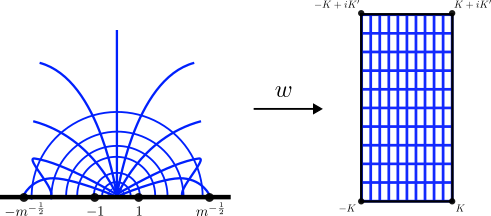
\includegraphics[width=0.72\linewidth]{img/SCR}
	\caption{Mapeo del semiplano superior a un rectángulo}
	\label{fig:scr}
\end{figure}
Rotamos y trasladamos el rectángulo para que sus vértices sean $w_1=-K+iK$, $w_2=-K$, $w_3=K$ y $w_4=K+iK$. Por simetría elegimos los $x_j$ como $z_1 = -m$, 
$z_2 = -1$, $z_3 = 1$ y $z_4 = m$,  donde $m$ es un parámetro que representa el grado de libertad en los $x_j$. La imagen del infinito resulta ser  el punto $iK'$, y la imagen de $0$ es $0$. La función puede escribirse como una integral elíptica de primera clase:
\[
\begin{array}{ccl}
	w&=&C_1\ds\int_{}^{z}\prod_{j=1}^{4}(t-x_j)^{-\frac{1}{2}}dt+C_2\\
	&=&-C_1\ds\int_{}^{z}\dfrac{dt}{\sqrt{(m^{2}-t^2)(1-t^2)}},
\end{array}
\]
resulta más conveniente hacer el cambio de variable $a=m^{-1}$, $C_1'=-C_1$, entonces 
\[
\begin{array}{ccl}
	w&=&C_1'\ds\int_{}^{z}\dfrac{dt}{\sqrt{(1-a^2t^2)(1-t^2)}}\\
	=&=&C_1'\ds\int_{}^{\sin^{-1}(z)}\dfrac{d\theta}{\sqrt{1-a^2\sin^2(\theta)}},
\end{array}
\]
Esta integral se conoce como integral elíptica incompleta de primera clase. \textbf{Mathematica} cuenta con una serie de funciones ya definidas para las integrales elípticas, en este ejemplo la función que usaremos seria \textbf{EllipticF[$\phi$, m]} la cual nos da la integral elíptica de primer orden $F(\phi|m)$.\\
Ingresando esta última integral en \textbf{Mathematica}
\begin{mmaCell}{Input}
	 Integrate[1/(Sqrt[1 - a*Sin[z]^2]), \{z, 0, ArcSin[z]\}]
\end{mmaCell}
obtenemos el siguiente resultado\\
\fbox{$F\left(\left.\sin ^{-1}(z)\right|a\right)\text{ if }0<\R\left(\sin ^{-1}(z)\right)\leq \dfrac{\pi }{2}\lor -\dfrac{\pi }{2}\leq \R\left(\sin ^{-1}(z)\right)<0$}\\
Para conocer más a detalle estas funciones en \textbf{Mathematica} vea \cite{Elliptic}.\\
Para simplificar este tomemos $c_1'=1$ y $m=2$, entonces $a=\dfrac{1}{2}$.
\begin{mmaCell}{Input}
	 ClearAll[z, w];\\w[z_] = EllipticF[ArcSin[z], 0.5^2];\\cartesianConformal[w[x + I*y], {x, -8, 8}, \{y, 10^(-12), 8\},\\Mesh -> 60, LabelStyle -> Directive[Larger, Bold],\\PlotStyle -> AbsoluteThickness[0.01], MeshStyle -> Blue,\\Axes -> True, PlotPoints -> 1000, PlotRange -> All]
\end{mmaCell}
\begin{mmaCell}[moregraphics={moreig={scale=0.8}}]{Output}
	\mmaFrac{ \mmaGraphics{31.png}}{}
\end{mmaCell}
\section{Ejemplos del uso de la fórmula de Schwarz-Christoffel para el disco unitario}
En este caso, podemos hacer uso de la simetría para considerar puntos $p_j$ que estén espaciados uniformemente alrededor del círculo unitario, incluso podemos tomar los puntos $_j$ de tal forma que sean las raíces $n$-ésimas de la unidad de
$$p_j=\omega_n^j,$$
$$\omega_n^{\frac{2\pi i}{n}}.$$
El producto $(p-p_1)\cdots (p-p_n)$ se simplifica a $p^n-1$. Tenemos por objetivo un $n$-ágono regular, los ángulos interiores para un $n$-ágono son todos iguales y están dados por:
$$\phi_k=\pi\left(1-\dfrac{2}{n}\right),$$
y los exponentes son todos iguales a $-\dfrac{2}{n}$. Por lo tanto, el mapeo deseado es de la forma 
\begin{equation}
	w=\bar{A}\ds\int \dfrac{dp}{(p^n-1)^{\frac{n}{2}}}+B.
\end{equation} 
Considerando los límites desde $p=0$ hasta $p=z$ y tomando $A=1$ obtendremos resultados más claros
\begin{equation}\label{SCn}
	w=\ds\int_{0}^{z}\dfrac{dp}{(1-p^n)^{\frac{n}{2}}}.
\end{equation}
\subsection{El hexágono}
Se obtiene un hexágono regular al establecer $n = 6$ en la ecuación (\ref{SCn}).
\begin{mmaCell}{Input}
  	 Integrate[1/(1 - p^6)^(1/3), {p, 0, z}]
\end{mmaCell} 
\vspace{-0.5 cm}donde obtenemos\\
\fbox{$z \, _2F_1\left(\dfrac{1}{6},\dfrac{1}{3};\dfrac{7}{6};z^6\right)\text{ if }-1<\text{Re} z\leq 1\lor z\notin \mathbb{R}$}\\
donde $_2F_1$ es la función hipergeométrica, en \textbf{Mathematica} esta función se escribe \textbf{ Hypergeometric2F1[a,b,c,z] }. Para más detalles puede consultar \cite{Hypergeometric2F1}.\\
Para comprobar qué está haciendo esta función usamos la función \textbf{polarConformal} que construimos anteriormente
\begin{mmaCell}{Input}
	 ClearAll[f, z]\\f[z_] = z Hypergeometric2F1[1/6, 1/3, 7/6, z^6]\\polarConformal[f[r Exp[I t]], {r, 0, 1},\\\{t, 0, 2*Pi\},Mesh -> \{50, 50\}, PlotRange -> All,\\LabelStyle -> Directive[Larger, Bold], PlotStyle -> White,\\MeshStyle -> Blue, Axes -> True]
\end{mmaCell}
\begin{mmaCell}[moregraphics={moreig={scale=0.8}}]{Output}
	\mmaFrac{ \mmaGraphics{32.png}}{}
\end{mmaCell}

\subsection{El $n$-ágono regular}
Con las consideraciones hechas previamente ahora nos resulta sencillo tratar el $n$-ágono regular
\begin{mmaCell}{Input}
	 nAgon[z_, n_] = Integrate[1/(1 - p^n)^(2/n), \{p, 0, z\},\\Assumptions -> n > 0]]
\end{mmaCell} 
obtenemos la siguiente expresión en términos de la función hipergeométrica
$$z \, _2F_1\left(\dfrac{1}{n},\dfrac{2}{n};1+\dfrac{1}{n};z^n\right).$$
Ahora, solo basta cambiar el parámetro $n$.\\
Las siguientes imágenes se generaron usando $n=3,4,5,10$ en el código
\begin{mmaCell}{Input}
	 ClearAll[f, z]\\polarConformal[nAgon[r Exp[I t], n], \{r, 0, 1\},\{t, 0, 2*Pi\},\\Mesh -> \{100, 100\}, PlotRange -> All,\\LabelStyle -> Directive[Larger, Bold],PlotStyle -> White,\\MeshStyle -> Blue, Axes -> True]
\end{mmaCell}
las imágenes obtenidas las podemos ver en la figura \ref{fig:Mapeo del círculo unitario al n-ágono}. \newpage
\begin{figure}[htbp]
	\centering
	\begin{subfigure}{0.45\textwidth}
		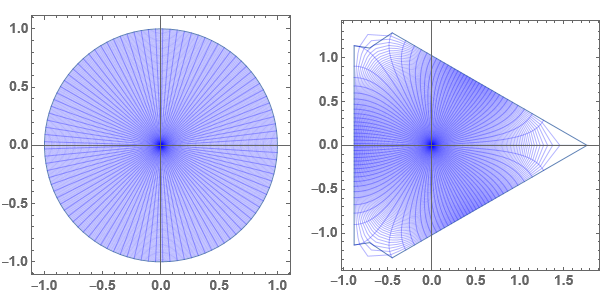
\includegraphics[width=\linewidth]{33.png}
		\caption{Mapeo del círculo unitario al triángulo.}
		\label{fig:Mapeo del círculo unitario al triángulo.}
	\end{subfigure}
	\begin{subfigure}{0.45\textwidth}
		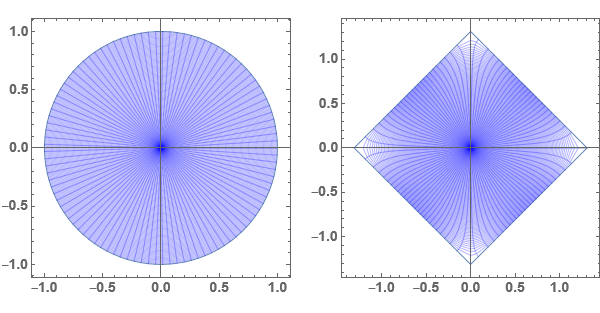
\includegraphics[width=\linewidth]{34.png}
		\caption{Mapeo del círculo unitario al cuadrado.}
		\label{fig:Mapeo del círculo unitario al cuadrado}
	\end{subfigure}
	
	\begin{subfigure}{0.45\textwidth}
		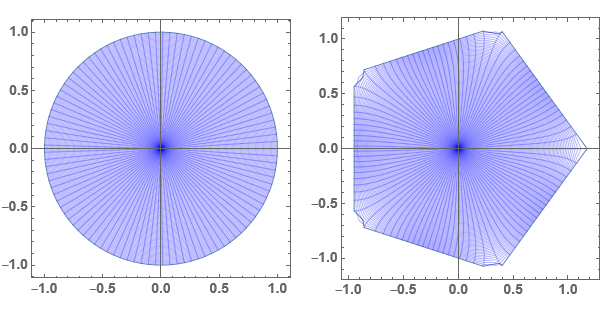
\includegraphics[width=\linewidth]{35.png}
		\caption{Mapeo del círculo unitario al pentágono.}
		\label{fig:Mapeo del círculo unitario al pentágono}
	\end{subfigure}
	\begin{subfigure}{0.45\textwidth}
		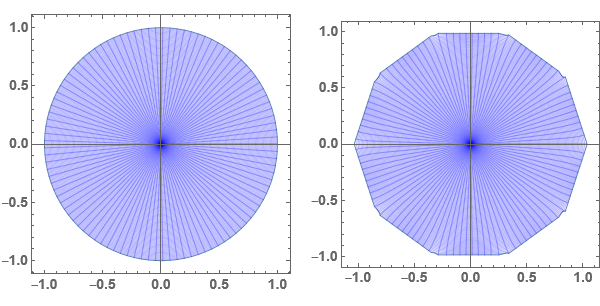
\includegraphics[width=\linewidth]{36.png}
		\caption{Mapeo del círculo unitario al decágono.}
		\label{fig:Mapeo del círculo unitario al decágono}
	\end{subfigure}
	\caption{Mapeo del círculo unitario al n-ágono}
	\label{fig:Mapeo del círculo unitario al n-ágono}
\end{figure}

\section{Miscelánea}
Sean $f\colon G\to\mathbb{C}$ una función,
$a$ un punto interior de $G$
y $r>0$ tal que la cerradura del disco $D(a,r)$ está contenida en $G$.
Definimos $A_{f,a,r}\colon[0,2\pi)\to\mathbb{R}$,
\[
A_{f,a,r}(\theta) = \operatorname{Arg}(f(a+re^{i\alpha})).
\]
\\
Teorema.
\\
Sea $f\colon G\to\mathbb{C}$ una función holomorfa
y sea $a$ un punto interior del dominio $G$.
Supongamos que $a$ es un cero de $f$ de orden $m$.
Entonces, existe $R>0$ tal que para cada $r$ que satisface $0<r<R$,
la función $A_{f,a,r}$ recorre $m$ veces los valores de $-\pi$ a $\pi$.








	
	\chapter{Aplicaciones} \label{Aplicaciones }

\section{Introducción}\label{intro_aplicaciones}

En el estudio de las matemáticas, uno encuentra resultados teóricos que son realmente fascinantes. Muchas veces, estos resultados fueron motivados por problemas prácticos. Solo por mencionar algunos de estos resultados, tendríamos el Teorema de Pitágoras y la ley de gravitación universal.\\
Además, está el estudio de esos números extraños que, en el siglo XVI, Rafael Bombelli los llamaba \capertura cantidad  salvaje'' y establecía las reglas de cálculo en su Álgebra. No fue sino hasta que Descartes los llamo \capertura números imaginarios'' y, posteriormente, Leonhard Euler introdujo la notación $i =\sqrt{-1}$, la cual ha aparecido en las ecuaciones de la mecánica cuántica y la transformada de Fourier.\\
Es por ello que, en este pequeño capítulo, presentamos algunos de los ejemplos donde podemos aplicar la teoría de los mapeos conformes a problemas físicos. 
\section{Flujo de fluidos}
Iniciamos esta sección presentando algunos conceptos clave que utilizaremos en el futuro. Es importante destacar que, para simplificar nuestra discusión, nos enfocaremos principalmente en el flujo de fluidos ideales.\\
Consideremos  un flujo de fluido ideal con el campo vectorial de velocidad
\[
	\textbf{v}=\left[\begin{array}{c}
		u(x,y)\\
		v(x,y)
	\end{array}\right]
\]
en el punto \[
\textbf{x}=\left[\begin{array}{c}
	x\\
	y\end{array}\right]
\]
donde $\textbf{v(x)}$ denota la velocidad instantánea del fluido en el punto $\textbf{x}\in \Omega\subset \R^{2}$. Diremos que el flujo es incompresible , es decir, el volumen del líquido no cambia si y sólo si 
\begin{equation}\label{ec3-1}
	\nabla \cdot \textbf{v} =\dpartial{u}{x}+\dpartial{u}{y}=0.
\end{equation}
Por otro lado, diremos que el fluido es irrotacional si

\begin{equation}\label{ec3-2}
	\nabla \times \textbf{v} =\dpartial{v}{x}-\dpartial{v}{y}=0.
\end{equation}
Un flujo diremos que es un flujo de fluido ideal si es incompresible e irrotacional. La mayoría de los líquidos y los gases se comportan como flujos ideales.\\
Note que las ecuaciones (\ref{ec3-1})-(\ref{ec3-1}) son casi idénticas a las ecuaciones de Cauchy-Riemann.\\ 
\noindent Tenemos el siguiente teorema
\begin{teor}
	El campo vectorial de velocidad $\textbf{v}=[u(x,y)\;\;\; v(x,y)]^{T}$ induce un flujo de fluido ideal si y sólo si
	\begin{equation}\label{ec3-3}
		f(z)=u(x,y)-iv(x,y),
	\end{equation}
	es una función analítica en $z=x+iy$.\endproof
\end{teor}
Note que los componentes $u$ y $-v$ del campo vectorial de velocidad para los flujos de fluidos ideales son necesariamente conjugados armónicos. La función $f(z)$ es conocida como la velocidad compleja del flujo de fluido. Bajo tal flujo, las partículas del fluido siguen las trayectorias $z(t) = x(t)+iy(t)$ obtenidas integrando el sistema de ecuaciones diferenciales ordinarias.
\begin{equation}\label{ec3-4}
	\derivada{x}{t}=u(x,y),\; \; \; \derivada{y}{t}=v(x,y),
\end{equation}
o en forma compleja 

\begin{equation}\label{ec3-5}
	\derivada{z}{t}=\overline{f(z)},
\end{equation}
donde las curvas parametrizadas por la solución $z(t)$ se conocen como líneas de corriente del flujo de fluido. Si la velocidad compleja $f(z_0)$ en un punto $z_0$ desaparece, entonces la solución $z(t) = z_0$ de la ecuación (\ref{ec3-5}) es constante y el punto $z_0$ es un punto de estancamiento del flujo.\\
En lo que respecta a Mathematica, estaremos utilizando el comando \textbf{ComplexVectorPlot}. 

\begin{Ejem}
	Sea $f(z)=1$. El vector velocidad $\textbf{v}=[1\;\;\;0]^{T}$. Entonces $\derivada{z}{t}=1$ ya que $\derivada{x}{t}=1$ y $\derivada{t}{t}=0$. Resolviendo $\derivada{z}{t}=1$ se obtiene $z(t)=t+z_0$, que Representa un flujo uniforme horizontal que se manifiesta a través de líneas rectas paralelas al eje real.\endproof
	\begin{mmaCell}{Input}
		ComplexVectorPlot[1, {z, -3 - 3 I, 3 + 3 I}]
	\end{mmaCell}
	\begin{mmaCell}[moregraphics={moreig={scale=0.3}}]{Output}
		\mmaFrac{ \mmaGraphics{37.png}}{}
	\end{mmaCell}
\end{Ejem}
\begin{Ejem}
	Sea $f(z)=c=a+bi$. Resolviendo $\derivada{z}{t}=\overline{c}=a-ib$, se tienen que $z(t)=\overline{c}t+z_0$. Las líneas de corriente son paralelas a las rectas inclinadas formando un ángulo $\theta=\operatorname{arg}(\overline{c})=\operatorname{arg}(c)$ al eje real. A continuación se muestra usando $a=3$ y $b=4$
	\begin{mmaCell}{Input}
		ComplexVectorPlot[3 + 4*I, {z, -3 - 3 I, 3 + 3 I}]
	\end{mmaCell}
	\begin{mmaCell}[moregraphics={moreig={scale=0.3}}]{Output}
		\mmaFrac{ \mmaGraphics{38.png}}{}
	\end{mmaCell}
\end{Ejem}


Supongamos ahora que la velocidad compleja $f(z)$ admite una antiderivada compleja, es decir, una
función analítica compleja $g(z)$ tal que 
\begin{equation}\label{ec3-6}
	g(z)=\phi(x,y)+i\psi(x,y),
\end{equation}
donde $\derivada{g}{z}=f(z)$.\\
Luego, de las ecuaciones de Cauchy-Riemann se sigue que
\[
\derivada{g}{z}=\dpartial{\phi}{x}-i\dpartial{\phi}{y}=u-iv \implies \dpartial{\phi}{x}=u,\; \dpartial{\phi}{y}=v.
\]
Entonces, $\nabla\phi=\textbf{v}$, y $\phi(x,y)=\operatorname{Re}\{g(x)\}$ define un potencial de velocidad del flujo de fluido. Por lo tanto, la función $g(z)$ es conocida como la función potencial compleja para el campo de velocidades dado. Luego $ \phi(x, y)$ es una función analítica y armónica que satisface la ecuación de Laplace $\nabla^{2}\phi= 0$. Por el contrario, cualquier función armónica puede considerarse como el potencial para algún flujo de fluido, donde la velocidad real del flujo es su gradiente $\textbf{v} = \nabla\phi$, representando así un flujo de fluido ideal. La función armónica $\phi(x, y)$ se conoce como función de corriente; esta cumple con la ecuación de Laplace, y las funciones de potencial y corriente están relacionadas a través de las ecuaciones de Cauchy-Riemann.
\begin{equation}\label{ec3-7}
	\dpartial{\phi}{x}=u=\dpartial{\psi}{y},\;\;\; \dpartial{\phi}{y}=v=-\dpartial{\psi}{x}.
\end{equation}
Los conjuntos de nivel del potencial de velocidad, definidos por $\{\phi(x,y)=c,\;c\in\R\}$, se conocen como curvas equipotenciales. El potencial de velocidad $\textbf{v}=\nabla \phi\neq 0$ es normal a las curvas equipotenciales. Notemos que, $\textbf{v}=\nabla \phi$ también es tangente a las curvas de nivel $\{\phi(x,y)=d\}$ de su función armónica conjugada. Pero $\textbf{v}$ al ser el campo de velocidad, es tangente a las líneas de corriente debidas a las partículas del fluido. Por lo que, estos dos sistemas de curvas deben ser iguales. Por lo tanto, las curvas de nivel de las líneas de corriente del flujo, y el conjunto de curvas equipotenciales $\{\phi=c\}$ y el conjunto de líneas de corriente $\{\psi=d\}$  son dos familias mutuamente ortogonales de curvas planas.  

\begin{Ejem}[Flujo alrededor de un disco]
	Considere la función potencial compleja
	$$g(z)=z+\dfrac{1}{z}=\left(x+\dfrac{x}{x^2+y^2}\right)+i\left(y-\dfrac{y}{x^2+y^2}\right),$$
	donde las partes real e imaginaria son soluciones de las ecuación de Laplace en dos dimensiones.  el  campo de flujo complejo correspondiente es 
	$$f(z)=\derivada{g}{z}=1-\dfrac{1}{z^2}=1-\dfrac{x^2-y^2}{(x^2+y^2)^2}+i\dfrac{2xy}{(x^2+y^2)}.$$
	Los puntos $z=\pm 1$ son puntos de estancamiento del flujo, y $z=0$ es una singularidad. Por lo tanto, el fluido que se mueve a lo largo del eje real positivo  se acerca al punto de estancamiento $z=-1$ cuando $t\rightarrow \infty$. Notemos que las líneas de corriente $\phi(x,y)=y-\dfrac{y}{x^2+y^2}=d$ se vuelven horizontales a medida que más se alejen del origen, es flujo es similar al un flujo horizontal uniforme, de izquierda a derecha, con velocidad compleja unitaria $f(z)=1$.
	
	Las curvas de nivel para $d = 0$ consisten en el círculo unitario $|z| = 1$ en el eje real. En particular, el círculo unitario consta de dos líneas de corriente semicirculares junto con dos puntos de estancamiento.
	La velocidad del flujo $\textbf{v} = \nabla\phi$ es tangente en todas partes al círculo unitario y, por lo tanto, satisface la condición $\mathbf{v}\cdot\mathbf{n}=0$ a lo largo de la frontera $|z|=1$.
	  
	Nuestro resultado en Mathematica 
	\begin{mmaCell}{Input}
		ComplexVectorPlot[z + (z/(z*z)), \{z, -3 - 3 I, 3 + 3 I\}, \\RegionFunction -> Function[\{z, f\}, Abs[z] > 1]]
	\end{mmaCell}
	\begin{mmaCell}[moregraphics={moreig={scale=0.3}}]{Output}
		\mmaFrac{ \mmaGraphics{39.png}}{}
	\end{mmaCell}
\end{Ejem}

\section{Transferencia de calor}
Los problemas de transferencia de calor pueden ser resueltos tanto por métodos analíticos como métodos usando mapeos conformes. Las trasformaciones conformes que se utilizan son
\begin{itemize}
	\item $z=\sen w$,
	\item $w=-i\dfrac{z-1}{z+1}$,
	\item $T=z^2$,
	\item  $w=i\log T=2i\log z$,
\end{itemize}
La ecuación de calor es 
\begin{equation}\label{ec3-8}
	u_t=ku_{xx}
\end{equation}
donde $k$ se le conoce como coeficiente de difusividad térmica.\\
A continuación se presentan algunos ejemplos que comúnmente se resuelven en un curso ordinario de ecuaciones diferenciales parciales (EDP) usando métodos analíticos.
\begin{Ejem}
	Considere la ecuación de calor 
	$$u_t=ku_{xx},\;\;\; -\infty<x<\infty,\;\;\;t>0$$
	Esta ecuación tiene los siguientes conjuntos de soluciones 
	\begin{itemize}
		\item [(i)] $u_0(x,t)=Ax+B$, donde $a$ y $B$ son constantes arbitrarias, y
		\item [(ii)]  $u_\lambda(x,t)=\cosh(\lambda x)e^{{k\lambda^2t}}$, donde $\lambda\in\R^{+}$.
	\end{itemize}
	Notemos que para cualquier $t$ fijo, 
	$$\lim_{x\rightarrow\pm\infty}u_\lambda(x,t)=+\infty$$
	Como estas soluciones no están acotadas cuando $x\rightarrow\pm\infty$, estas no son aceptables para problemas físicos. Si se requiere que la solución $u$ sea acotada en el infinito tanto en $x$ como en $t$, debemos  de establecer las siguientes condiciones 
	\[
	\begin{array}{ccc}
		\ds\lim_{x\rightarrow\pm\infty}u(x,t)<\infty,&&\ds\lim_{t\rightarrow\infty}u(x,y)<\infty,
	\end{array}
	\]
	así como la condición inicial $u(x,0)=f(x)$, $-\infty<x<\infty$, donde $f(x)$ es una función acotada para todo $x$.\endproof
\end{Ejem}
\begin{Ejem}
	Considere la ecuación de calor 
	$$u_t=ku_{xx},\;\;\; 0<x<l$$
	sujeta a las condiciones iniciales y de frontera
	\[
	\begin{array}{cccc}
		u(0,t)=0=u(l,t),& t>0,&u(x,0)=f(x),&0<x<l,
	\end{array}
	\]
	donde $f\in C^{1}$. En términos físicos, este problema representa la conducción de calor en una varilla cuando sus extremos se mantienen a temperatura cero mientras que la temperatura inicial $u$ en cualquier punto de la varilla esta dada por $f(x)$. Usando el método de separación de variables y las condiciones anteriores, la solución es
	$$u(x,t)=\sum_{n=1}^{\infty}C_n\sen \left(\dfrac{n\pi x}{l}\right)e^{\frac{-kn^2 \pi^2 t}{l^2}},$$
	donde $$C_n=\dfrac{2}{l}\int_{0}^{l}f(x)\sen\left(\dfrac{n\pi x}{l}\right)dx,\;\;\;n=1,2,3,\ldots$$\endproof
\end{Ejem}
\begin{Ejem}
	Considere la ecuación de calor 
	$$u_t=u_{xx},\;\;\; 0<x<1$$
	sujeta a las condiciones iniciales y de frontera
	\[
	\begin{array}{ccccc}
		u(0,t)=1,&u(1,t)=0,&t>0& u(x,0)=0,&0<x<1
	\end{array}
	\]
	En este ejemplo, primero encontremos una solución particular, para ello podemos tomar el caso de estado estacionario, donde la ecuación se convierte en $\tilde{u_{xx}}=0$, la cual al integrar dos veces se obtiene la solución general
	$$\tilde{u}(x)=c_1x+c_2.$$
	Luego, usando las condiciones de frontera $\tilde{u}(0)=1$, $\tilde{u}(1)=0$ obtenemos la solución en el estado estacionario $$\tilde{u}(x)=1-x.$$
	A continuación, formulamos un problema homogéneo escribiendo $u(x, t)$ como una suma de la solución de estado estacionario $\tilde{u}(x)$ y un término transitorio $v(x,t)$, es decir, $u(x,t)=\tilde{u}(x)+v(x,t)$ o 
	$$v(x,t)=u(x,t)-\tilde{u}(x).$$
	Sustituyendo esta ecuación en el problema original se obtiene 
	$$v_t=v_{xx},$$
	donde las condiciones de frontera e iniciales se reducen a 
	\[
	\begin{array}{c}
		v(0,t)=u(0,t)-\tilde{u}(0)=0\\
		v(1,t)=u(1,t)-\tilde{u}(1)=0\\
		v(x,0)=u(x,0)-\tilde{u}(x)=x-1
	\end{array}
	\]
	Resolviendo esta EDP se obtiene 
	$$v(x,t)=\sum_{n=1}^{\infty}C_ne^{-n^2\pi^2t}\sen n\pi x,$$
	donde $$C_n=2\int_{0}^{1}(x-1)\sen n\pi x dx=-\dfrac{2}{n\pi}.$$
	Luego $$v(x,t)=-\dfrac{2}{\pi}\sum_{n=1}^{\infty}\dfrac{1}{n}e^{-n^2\pi^2t}\sen n\pi x,$$
	Por lo tanto 
	$$u(x,t)=1-x-\dfrac{2}{\pi}\sum_{n=1}^{\infty}\dfrac{1}{n}e^{-n^2\pi^2t}\sen n\pi x.$$\endproof
\end{Ejem}
Los siguientes ejemplos se resuelven usando transformaciones conformes 
\begin{Ejem}
	Considere el caso de la distribución de temperatura en las regiones semicirculares superior e inferior del disco unitario con la temperatura en la frontera dada por
	\[
	u=\left\{
	\begin{array}{ccc}
		20^{\circ}&\mbox{si}& \theta\in(0,\pi)\\
		0^{\circ}&\mbox{si}&\theta\in (-\pi,0)
	\end{array}
	\right.
	\]
	Para encontrar la temperatura en los puntos $z=0$ y $z=\dfrac{1}{2}$, usaremos la función $$\zeta=i\dfrac{1-z}{1+z},$$ esta función mapea la región $|z|<1$ en el semiplano superior del plano $\zeta$, de modo que la frontera superior del disco unitario se mapee en el eje positivo $\xi$ mientras que la frontera inferior se mapee en  el eje negativo $\xi$ (vea la Figura \ref{fig:40}).
	\begin{figure}
		\centering
		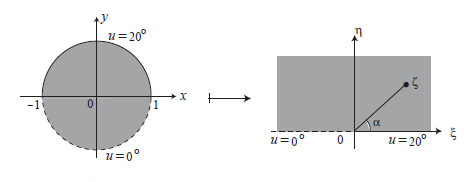
\includegraphics[width=0.7\linewidth]{img/40}
		\caption{Mapeo del círculo al semiplano superior}
		\label{fig:40}
	\end{figure}
	Entonces la distribución de la temperatura en el plano $\zeta$ esta dada por $u=A\alpha+B$, donde $\alpha=\arctan(\eta/\xi)$, donde $\arctan(\eta/\xi) \in [0,\pi]$, de las condiciones de frontera se tiene $B=20$ y $A=-20/\pi$, por lo tanto,
	\begin{equation}\label{ec3-9}
		u=-\dfrac{20}{\pi}\arctan(\eta/\xi)+20,
	\end{equation}
	si usamos la función $\zeta=-i\dfrac{z-1}{z+1}$ obtenemos 
	$$\xi+i\eta=-i\dfrac{x-1+iy}{x+1+iy}=-i\dfrac{x^2+y^2-1+2iy}{(x+1)^2+y^2}.$$
	Igualando las partes reales e imaginarias se tiene que 
	\begin{equation}\label{ec3-10}
		\xi=\dfrac{2y}{(x+1)^2+y^2},\;\;\;\eta=\dfrac{1-x^2-y^2}{(x+1)^{2}+y^2}.
	\end{equation}
	Sustituyendo (\ref{ec3-10}) en (\ref{ec3-9}) obtenemos las distribución de la temperatura
	\begin{equation}\label{ec3-11}
		u(x,y)=-\dfrac{20}{\pi}\arctan\left(\dfrac{1-x^2-y^2}{2y}\right)+20.
	\end{equation}
	Entonces, la temperatura en $z=0$ es 
	$$u(0,0)=-\dfrac{20}{\pi}\arctan(\infty)+20=-\dfrac{20}{\pi}\dfrac{\pi}{2}+20=10^{\circ}$$
	ya que $\tan(\pi/2)=\infty$, y la temperatura en $(0,1/2)$ es
	$$u\left(0,\dfrac{1}{2}\right)=-\dfrac{20}{\pi}\arctan\left(\dfrac{3}{4}\right)+20\approx16.9^{\circ}.$$\endproof
\end{Ejem}

\section{Campo electromagnético}
Imagine un alambre conductor ortogonal al plano $z$ en el origen, sobre el cual se distribuye uniformemente una carga eléctrica de densidad $q$ unidades de carga en el alambre. El potencial eléctrico generado por este cable es $u = -2q \log r$, y el potencial complejo es
\begin{equation}\label{ec3-12}
	f(z)=2q\log z,
\end{equation}
esto debido a que en general, una linea de carga $q$ por unidad de longitud esta sujeta a la fuerza $q\mathbf{E}$ por unidad de longitud, donde $\mathbf{E}$ es el vector que describe la intensidad del campo eléctrico, el cual esta definido por 
\begin{equation}\label{ec3-13}
	\textbf{E}=-\nabla u, \;\; \mbox{ y }\;\; \textbf{E}=-\overline{f'(z)}
\end{equation} 
\begin{Ejem}
	Sea $q_1$ una carga por unidad de longitud en $z=0$ y sea $q_2$ otra carga por unidad de longitud en $z=1$. Entonces de (\ref{ec3-11}) el potencial complejo esta dado por la suma de los potenciales debido a las fuentes en $z=0$ y $z=1$, es decir,
	\begin{equation}\label{ec3-14}
		f(z)=-2q_1\log z-2q_2\log (z-1).
	\end{equation}
	Dado que el potencial $u=\operatorname{Re}(f(z))$, tenemos que 
	\[
	\begin{array}{ccl}
		u&=&-2q_1\ln |z|-2q_2\ln|z-1|\\
		&=&-2q_1\ln\sqrt{x^2+y^2}-2q_2\ln\sqrt{(x-1)^2+y^2}\\
		&=&-q_1\ln(x^2+y^2)-q_2\ln((x-1)^2+y^2).
	\end{array}
	\]
	De (\ref{ec3-13}) tenemos que 
	$$\mathbf{E}=-\overline{f'(z)}=-(\overline{-2(q_1\ln|z_1|+q_2\ln|z-1|)'})=2\left(\overline{q_1\dfrac{1}{z}+q_2\dfrac{1}{z-1}}\right)=\dfrac{2q_1}{\bar{z}}+\dfrac{2q_2}{\bar{z}-1}$$
	
\end{Ejem}
Cuando $$\operatorname{Im}(f(z))=v=c,$$ donde $c$ es constante, las líneas $v=c$ son llamadas lineas de fuerza y el vector $\mathbf{E}$ es tangente a estas líneas.\\
En el ejemplo anterior, si $q_1=q_2=q-2q\ln|z(z-1)|-2qi\operatorname{arg}\{z(z-1)\}$ y como $\operatorname{arg}\{z(z-1)\}=\dfrac{2xy-y}{x^2-y^2-x}$, la parte imaginaria del potencial complejo es dada por 
$$v(x,y)=-2q\arctan\dfrac{2xy-y}{x^2-y^2-x},$$
y entonces, las líneas de fuera, definidas por $v=c$, son dadas por 
$$\dfrac{2xy-y}{x^2-y^2-x}=\tan\left(-\dfrac{c}{2q}\right)=C$$
donde $C$ es una constante.\\ Las líneas de fuerza $v=c$, en los puntos $z=\pm 1$ se muestran en la a continuación.
\begin{mmaCell}{Input}
	 Show[StreamPlot[\{(2*x*y - y)/(x^2 + y^2 - x), 1.0\},\\\{x, -10, 10\}, \{y, -10, 10\}],ListPlot[\{\{-1, 0\}, \{1, 0\}\}, \\PlotStyle -> Red]]
\end{mmaCell}

\begin{mmaCell}[moregraphics={moreig={scale=0.3}}]{Output}
	\mmaFrac{ \mmaGraphics{41.png}}{}
\end{mmaCell}

\printbibliography[heading=bibintoc]
	
	%\chapter{Modelación espacio-temporal} \label{chap:modeling}

\section{Modelos espaciales} \label{sec:spatial_models}

\subsubsection{Modelo Poisson-Gamma} \label{subsubsec:bayesian_poisson_gamma}


	
	%\chapter{Conclusiones y trabajo futuro}
		% Apendice
%	\appendix
%	\chapter{Anexo}
	% Referencias
	%\bibliographystyle{ieeetr}  
	
	\nocite{tarlok}
	\nocite{silverman}
	\nocite{shaw}
	\nocite{ComplexRegionPlot}
	\nocite{marsden}
	\nocite{Churchill}
	\nocite{ahlfors}
	\nocite{rajeev}
	\nocite{Driscoll}
	\nocite{Abramowitz}
	\nocite{Beta}
	\nocite{BetaInc}
	\nocite{Pearson}
	\nocite{BetaR}
	\nocite{Conway}
	\nocite{Elliptic}
	\nocite{Hypergeometric2F1}
	\nocite{ComplexPlot}
	\nocite{ComplexPlot3D}
	\nocite{ComplexContourPlot}
	\nocite{Shaw-A}
	\nocite{GeometryJo}
	\nocite{ComplexVector}
	\nocite{Domain_coloring}
%\printindex
%	\backmatter
	
\end{document}

% LaTeX references (technical issues, workarounds)

% https://www.overleaf.com/learn/latex/Management_in_a_large_project ('including files' section)
% https://tex.stackexchange.com/questions/64839/how-to-change-listing-caption
% https://stackoverflow.com/questions/2709898/change-list-of-listings-text
% https://tex.stackexchange.com/questions/664/why-should-i-use-usepackaget1fontenc